\documentclass[11pt,]{tufte-book}

% ams
\usepackage{amssymb,amsmath}

\usepackage{ifxetex,ifluatex}
\usepackage{fixltx2e} % provides \textsubscript
\ifnum 0\ifxetex 1\fi\ifluatex 1\fi=0 % if pdftex
  \usepackage[T1]{fontenc}
  \usepackage[utf8]{inputenc}
\else % if luatex or xelatex
  \makeatletter
  \@ifpackageloaded{fontspec}{}{\usepackage{fontspec}}
  \makeatother
  \defaultfontfeatures{Ligatures=TeX,Scale=MatchLowercase}
  \makeatletter
  \@ifpackageloaded{soul}{
     \renewcommand\allcapsspacing[1]{{\addfontfeature{LetterSpace=15}#1}}
     \renewcommand\smallcapsspacing[1]{{\addfontfeature{LetterSpace=10}#1}}
   }{}
  \makeatother
\fi

% graphix
\usepackage{graphicx}
\setkeys{Gin}{width=\linewidth,totalheight=\textheight,keepaspectratio}

% booktabs
\usepackage{booktabs}

% url
\usepackage{url}

% hyperref
\usepackage{hyperref}

% units.
\usepackage{units}


\setcounter{secnumdepth}{2}

% citations

% pandoc syntax highlighting

% longtable
\usepackage{longtable,booktabs}

% multiplecol
\usepackage{multicol}

% strikeout
\usepackage[normalem]{ulem}

% morefloats
\usepackage{morefloats}


% tightlist macro required by pandoc >= 1.14
\providecommand{\tightlist}{%
  \setlength{\itemsep}{0pt}\setlength{\parskip}{0pt}}

% title / author / date
\title{Major Area Paper\\
(v8.1)}
\author{Rachel M. Smith}
\date{16 June 2017}

% \usepackage{caption}
% \usepackage{cleveref}
% \usepackage{biblatex}
% \renewbibmacro*{date}{%
%    \printdate
%    \iffieldundef{origyear}{%
%    }{%
%      \setunit*{\addspace}%
%      \printtext[parens]{\printorigdate}%
%    }%
% }

%
% --------------------- %
% Latex Logo Commands
% --------------------- %
%
\usepackage{xspace}
\newcommand{\latex}{\LaTeX\xspace}
\newcommand{\tex}{\TeX\xspace}
\newcommand{\bibtex}{\textsc{Bib}\tex}
%
% --------------------- %
% Colors
% --------------------- %
%
\usepackage{xcolor}
\usepackage{color}
\definecolor{magenta}{rgb}{0.79, 0.08, 0.48} %% ~c9147a %%
\definecolor{dkmagenta}{rgb}{0.55, 0.0, 0.55} %% ~8c008c %%
\definecolor{dpmagenta}{rgb}{0.8, 0.0, 0.8} %% ~140014 %%
\definecolor{patriarch}{rgb}{0.5, 0.0, 0.5} %% ~0d000d %%
\definecolor{dkpatriarch}{rgb}{0.4, 0.0, 0.4} %% ~0a000a %%
\definecolor{blue}{rgb}{0.07, 0.04, 0.56} %% ~120a8f %%
\definecolor{royalblue}{rgb}{0.0, 0.22, 0.66} %% ~0038a8 %%
\definecolor{dkblue}{rgb}{0.0, 0.0, 0.55} %% ~00008c %%
\definecolor{mnblue}{rgb}{0.1, 0.1, 0.44} %% ~030370 %%
\definecolor{smblue}{rgb}{0.0, 0.2, 0.6} %% ~00050f %%
\definecolor{Rblue}{rgb}{0.39, 0.35, 0.639} %% ~0a09a3 %%
\definecolor{dkmnblue}{rgb}{0.0, 0.2, 0.4} %% ~00050a %%
\definecolor{navy}{rgb}{0.0, 0.0, 0.5} %% ~00000d %%
\definecolor{dknavy}{rgb}{0, 0, .208} %% ~000035 %%
\definecolor{blublk}{rgb}{0, 0, .106} %% ~00001b %%
\definecolor{blugray}{rgb}{0.33, 0.41, 0.47} %% ~546978 %%
\definecolor{grayblue}{rgb}{0.33, 0.41, 0.58} %% ~~546994 %%
\definecolor{slgray}{rgb}{0.44, 0.5, 0.56} %% ~70808d %%
\definecolor{red}{rgb}{.545, 0.0, 0.0} %% ~8b0000 %%
\definecolor{dkred}{rgb}{.247, 0.0, 0.0} %% ~3f0000 %%
\definecolor{mplblu}{HTML}{363283}
%
\definecolor{pdxgray}{HTML}{373737} %% ~373737 %%
\definecolor{pdxgreen}{HTML}{8B9535} %% ~8B9535 %%
\definecolor{myblack}{HTML}{181C20} %% ~181C20 %%
%
% ---------------------------------------- %
% Indent first line of text in tabular env %
% ---------------------------------------- %
%
\newcommand{\rowgroup}[2][-1em]{\hspace{#1}#2}
\newcommand{\mrowgroup}[3]{\hspace*{#1}#2\hspace*{#1}#3}
%
% --------------------- %
% Format Block Quotes
% --------------------- %
%   Size: Scriptsize
%   Reduce vertical space above
%   Color: Gray
%
\usepackage{setspace}
% \expandafter\def\expandafter\quote\expandafter{\quote\small\singlespacing\color{myblack!65}\vspace{-0.5\baselineskip}}

% \expandafter\def\expandafter\quote\expandafter{\quote\small\singlespacing\vspace{-1em}}

% \setlength\listindent{1em}

\usepackage{enumitem}
% \setlist[itemize, 1]{leftmargin=!, labelindent=0.5em, itemindent=-3em, label=\scriptsize{$\cdot$}, partopsep=0em, topsep=0.15em}
% \setlist[itemize, 2]{leftmargin=4em, label=$\centerdot$, topsep=0em}
% \setlength{\itemindent}{5in}

%
% ------------------- %
% Make Links Standout
% ------------------- %
%   (E.Tufte does not believe in using colors in links. I disagree.) %
%
% \newcommand{\rurl}[1]{\underline{\color{dkblue}{\url{~1}}}}
% \newcommand{\rhref}[2]{\underline{\color{dkblue}{\href{~1}{~2}}}}
\hypersetup{breaklinks=true,colorlinks=true,linkcolor=navy,urlcolor=navy}
%
% ------------------- %
% Format "texttt"
% ------------------- %
%
\newcommand{\rtt}[1]{\color{patriarch}{\texttt{#1}}}
%
\usepackage{amsmath}

\usepackage{enumitem,amssymb}
\newlist{todolist}{itemize}{2}
\setlist[todolist]{label=$\square$}
\newcommand{\todoitem}[1]{\textit{\color{red}{#1}}}

\newcommand{\textbft}[1]{\underline{\textbf{\texttt{#1}}}}


% ---------------------------%
% Code Formatting %
% ---------------------------%
% \usepackage{highlight}

% \definecolor{fgcolor}{rgb}{0.196, 0.196, 0.196}
% \newcommand{\hlnum}[1]{\textcolor[rgb]{0.063,0.58,0.627}{#1}}%
% \newcommand{\hlstr}[1]{\textcolor[rgb]{0.063,0.58,0.627}{#1}}%
% \newcommand{\hlcom}[1]{\textcolor[rgb]{0.588,0.588,0.588}{#1}}%
% \newcommand{\hlopt}[1]{\textcolor[rgb]{0.196,0.196,0.196}{#1}}%
% \newcommand{\hlstd}[1]{\textcolor[rgb]{0.196,0.196,0.196}{#1}}%
% \newcommand{\hlkwa}[1]{\textcolor[rgb]{0.231,0.416,0.784}{#1}}%
% \newcommand{\hlkwb}[1]{\textcolor[rgb]{0.627,0,0.314}{#1}}%
% \newcommand{\hlkwc}[1]{\textcolor[rgb]{0,0.631,0.314}{#1}}%
% \newcommand{\hlkwd}[1]{\textcolor[rgb]{0.78,0.227,0.412}{#1}}%

\let\hlipl\hlkwb
% \newcommand{\Rrule}{\textcolor{Rblue}{\rule{\linewidth}{0.05mm}}\newline
\includegraphics[width=0.5cm]{auxDocs/Rlogo.png}}
\usepackage{dashrule}

\newcommand{\Rrule}{
    % \setlength{\parindent}{-10pt}
    \vspace*{1em}
    \noindent
    \hspace{-1em}
    
\includegraphics[width=0.5cm]{auxDocs/Rlogo.png}
    \textcolor{Rblue}{
        \rule[0.1in]{0.90\linewidth}{0.02mm}
    }
    \vspace{-1.35em}
}

\newcommand{\Rerule}{
    % \setlength{\parindent}{-0.5in}
    \noindent
    \hspace{-1em}
    \textcolor{Rblue}{
        $\llcorner$\rule[-0.4mm]{\linewidth}{0.02mm}
                % \hfill
                % $\lrcorner$
    }
}

\newcommand{\Rruleb}{
    % \setlength{\parindent}{-10pt}
    \vspace*{1em}
    \noindent
    \hspace{-1em}
    
\includegraphics[width=0.5cm]{auxDocs/Rlogo-bw.png}
    \textcolor{slgray}{
        \rule[0.1in]{0.90\textwidth}{0.02mm}
    }
    \vspace{-1.35em}
}

\newcommand{\Reruleb}{
    % \setlength{\parindent}{-0.5in}
    \noindent
    \hspace{-1em}
    \textcolor{slgray}{
        $\llcorner$\rule[-0.4mm]{\textwidth}{0.02mm}
                % \hfill
                % $\lrcorner$
    }
}

\newcommand{\MPrule}{
    % \setlength{\parindent}{-10pt}
    \vspace*{1em}
    \noindent
    \hspace{-1em}
    
\includegraphics[width=0.5cm]{../auxDocs/mplus.png}
    \textcolor{mplblu}{
        \rule[0.1in]{0.90\textwidth}{0.02mm}
    }
    \vspace{-1.5em}
}

\newcommand{\MPerule}{
    % \setlength{\parindent}{-0.5in}
    \noindent
    \hspace{-1em}
    \textcolor{mplblu}{
        $\llcorner$\rule[-0.4mm]{\textwidth}{0.02mm}
                % \hfill
                % $\lrcorner$
    }
}

\newcommand{\Frule}{
    \vspace*{-1em}
    \begin{fullwidth}\textcolor{blublk}{\rule{\linewidth}{0.2mm}}\end{fullwidth}
}

\newcommand{\Frnp}{
    \vspace*{-1em}
    \begin{fullwidth}\textcolor{blublk}{\rule{\linewidth}{0.2mm}}\end{fullwidth}
    \newpage
}

\newcommand{\Fbrule}{ %% for tufte book format %%
    \vspace*{-4em}
    \begin{fullwidth}\textcolor{blublk}{\rule{\linewidth}{0.2mm}}\end{fullwidth}
}


\newcommand{\SFrule}[1][0.1mm]{
    \begin{fullwidth}\textcolor{blublk}{\rule{\linewidth}{#1}}\end{fullwidth}
}

% \newcommand{\Rrule}{
%     \noindent
%     \textcolor{Rblue}{
%         $\ulcorner\textregistered$\hdashrule[0.015in]{
%             0.9\linewidth
%             }
%             {1pt}{1pt}
%         $\textregistered\urcorner$
%         }}
% \newcommand{\Rerule}{
%     \noindent
%     \textcolor{Rblue}{
%         $\llcorner\textregistered$\hdashrule[0.025in]{
%             0.9\linewidth
%             }
%             {1pt}{1pt}
%         $\textregistered\lrcorner$
%         }}
% \newcommand{\Rerule}{\noindent\textcolor{Rblue}{\vdash\hdashrule[-0.015in]{\linewidth}{1pt}{1pt}\dashv}

% \vdash - \dashv
% \perp
% \ll - \gg
% +
% \pm
% \mp
% \ \newcommand{\Rrule}{\noindent
\includegraphics[width=0.5cm]{auxDocs/Rlogo.png}\textcolor{Rblue}{\hdashrule[0.25in]{\linewidth}{1pt}{1pt}}}
% \newcommand{\Rrule}{\noindent
\includegraphics[width=0.5cm]{auxDocs/Rlogo.png}\textcolor{Rblue}{\rule[0.25in]{\linewidth}{0.05mm}}}

% \newcommand{\Rerule}{\textcolor{Rblue}{\rule{\linewidth}{0.05mm}}}
% \hdashrule [⟨raise⟩] [⟨leader⟩] {⟨width⟩} {⟨height⟩} {⟨dash⟩}

%%%%%%%%%%%%%%%%%%%%%%%%%%
% Wrapper for Chi-Square %
%%%%%%%%%%%%%%%%%%%%%%%%%%

\newcommand{\tdef}[3][-0.5em]{\tufteskip\noindent\rowgroup[#1]{\textsc{#2}} \newline {#3}}
\newcommand{\hf}{\hfill}
\DeclareMathAlphabet{\mathpzc}{OT1}{pzc}{m}{it} %% to make \mathpzc typeset its argument in Zapf Chancery (see page 16 of "The Great, Big List of LATEX Symbols" by David Carlisle, Scott Pakin, & Alexander Holt (2001)) %%

\newcommand{\chisq}{\mathpzc{\chi^{2}}}

\newcommand{\sq}{^{2}}

\newcommand{\df}{\mathpzc{df}} %% degrees of freedom (df) %%

%
% ----------------------------- %
% Command to insert "ToDo" tags
% ----------------------------- %

\newcommand{\todo}{
    \textsuperscript{
        \tiny{
            \fcolorbox{dkred}{black!10}{
                \color{red}{
                    \textbf{\texttt{[ToDo]}}
                }
            }
        }
    }
}

\newcommand{\inprogress}{
    \textcolor{blue}{
        \textbf{\textit{\texttt{[In Progress]}}}
    }
}

\newcommand{\complete}{
    \sout{
        \textcolor{slgray}{
            \textit{\texttt{[Complete]}}
        }
    }
}

\newcommand{\edit}[1]{
    \textcolor{red}{
        \texttt{#1}
    }
}

\newcommand{\todot}{
    \textcolor{red}{\Large{$\mathbf{^{\otimes}}$}}
}
%%%%%%%%%%%%%%%%%%%%%%%%%%%%%%%%%%%%%%%%%%%%%%%%%%%%%%%%%%%%%%%%%%%%%%%%%%%%%%%%%%%%

% \usepackage{wrapfig}

%%%%%%%%%%%%%%%%%%%%%%%%%%%%%%%%%%%%%%%%%%%%%%%%%%%%%%%%%%%%%%%%%%%%%%%%%%%%%%%%%%%%
%% Hanging indent for reference lists

\newcommand{\refs}{
    \parindent=-1.7em\
    \
    \setlength{\parskip}{0.5\baselineskip}
}

%%%%%%%%%%%%%%%%%%%%%%%%%%%%%%%%%%%%%%%%%%%%%%%%%%%%%%%%%%%%%%%%%%%%%%%%%%%%%%%%%%%%
%% Change fontsize definitions
%% (source=https://tex.stackexchange.com/a/48212)

\makeatletter
\newcommand\semiHuge{\@setfontsize\semiHuge{20.82}{24.98}}
\makeatother

\makeatletter
\newcommand\LArge{\@setfontsize\LArge{17.35185}{20.82}}
\makeatother
%%%%%%%%%%%%%%%%%%%%%%%%%%%%%%%%%%%%%%%%%%%%%%%%%%%%%%%%%%%%%%%%%%%%%%%%%%%%%%%%%%%%


%%%%%%%%%%%%%%%%%%%%%%%%%%%%%%%%%%%%%%%%%%%%%%%%%%%%%%%%%%%%%%%%%%%%%%%%%%%%%%%%%%%%
%% Modify section heading style
%% (source=https://tex.stackexchange.com/a/36611)

% \titleformat{\section}
%   {\normalfont\LARGE\scshape\color[HTML]{5b0057}}{\thesection}{1em}{}
\titleformat{\section}
  {\normalfont\LARGE\itshape\color{dknavy}}{\thesection}{1em}{}
\hypersetup{colorlinks,
            linkcolor=dknavy}

%%%%%%%%%%%%%%%%%%%%%%%%%%%%%%%%%%%%%%%%%%%%%%%%%%%%%%%%%%%%%%%%%%%%%%%%%%%%%%%%%%%%
%% Headers and footers
%% (source-1=https://groups.google.com/forum/#!topic/tufte-latex/b5Aj7sWeaBU)
%% (source-2=https://www.sharelatex.com/learn/Headers_and_footers)
%
% \let\runauthor\@author
% \let\runtitle\@title

\newcommand{\changefont}{%
    \fontsize{7}{9.5}\selectfont
}

\usepackage{fancyhdr}
% \fancypagestyle{plain}{
% \fancyhead[LO,LE]{\changefont Riley M. Smith}
% \fancyhead[RO,RE]{\changefont \thepage}
% \fancyhead[CO,CE]{\changefont @title}
% \fancyhead[LO,RE]{Riley M. Smith}
% \fancyhead[RO,RE]{\thepage}
% \fancyhead[CO,CE]{
\includegraphics[width=1cm]{graphics/inputs/compsLogo-tiny.png}}
% \fancyfoot[CO,CE]{\changefont \today}
% \fancyfoot[CO,CE]{\medskip\changefont\today}
\renewcommand{\headrulewidth}{0pt}
\renewcommand{\footrulewidth}{0pt}
% }
% \pagestyle{plain}
%%%%%%%%%%%%%%%%%%%%%%%%%%%%%%%%%%%%%%%%%%%%%%%%%%%%%%%%%%%%%%%%%%%%%%%%%%%%%%%%%%%%

\geometry{
          bottom=0.65in,
        %   top=1in,
          headsep=0.5in
}

% Make lists without bullets
% \renewenvironment{itemize}{
%   \begin{list}{}{
%     \setlength{\leftmargin}{1.5em}
%     \setlength{\parskip}{0.15\baselineskip}
%   }
% }{
%   \end{list}
% }
\setcounter{secnumdepth}{0}

\setsidenotefont{\scriptsize\color{dknavy}}
\setcaptionfont{\footnotesize\color{dknavy}}
\setmarginnotefont{\scriptsize\color{dknavy}}
% \setcitationfont{⟨font commands⟩}

\begin{document}

\maketitle



{
\setcounter{tocdepth}{1}
\tableofcontents
}

% pandoc-xnos: macro to create a caption without a prefix
\makeatletter
\def\LT@makenoprefixcaption#1#2#3{%
  \LT@mcol\LT@cols c{\hbox to\z@{\hss\parbox[t]\LTcapwidth{
    \sbox\@tempboxa{#1{}#3}
    \ifdim\wd\@tempboxa>\hsize
      #1{}#3
    \else
      \hbox to\hsize{\hfil\box\@tempboxa\hfil}%
    \fi
    \endgraf\vskip\baselineskip}
  \hss}}}
\makeatother

% pandoc-tablenos: save original macros
\makeatletter
\let\LT@oldmakecaption=\LT@makecaption
\let\oldthetable=\thetable
\let\oldtheHtable=\theHtable
\makeatother

% pandoc-tablenos: environment disables table caption prefixes
\makeatletter
\newcounter{tableno}
\newenvironment{no-prefix-table-caption}{
  \let\LT@makecaption=\LT@makenoprefixcaption
  \renewcommand\thetable{x.\thetableno}
  \renewcommand\theHtable{x.\thetableno}
  \stepcounter{tableno}
}{
  \let\thetable=\oldthetable
  \let\theHtable=\oldtheHtable
  \let\LT@makecaption=\LT@oldmakecaption
  \addtocounter{table}{-1}
}
\makeatother

% pandoc-xnos: cleveref fakery
\newcommand{\plusnamesingular}{}
\newcommand{\starnamesingular}{}
\newcommand{\xrefname}[1]{\protect\renewcommand{\plusnamesingular}{#1}}
\newcommand{\Xrefname}[1]{\protect\renewcommand{\starnamesingular}{#1}}
\providecommand{\cref}{\plusnamesingular~\ref}
\providecommand{\Cref}{\starnamesingular~\ref}
\providecommand{\crefformat}[2]{}
\providecommand{\Crefformat}[2]{}

% pandoc-xnos: cleveref formatting
\crefformat{table}{Table~#2#1#3}
\Crefformat{table}{Table~#2#1#3}
\crefformat{figure}{Figure~#2#1#3}
\Crefformat{figure}{Figure~#2#1#3}

\Frule

\chapter{Introduction}\label{introduction}

The purpose of this review is to provide a systematic methodological
overview and critique of the available empirical research related to
intimate partner violence (IPV) intervention and prevention efforts
through a community psychological lens. This review is specifically
focused on the applied methodologies employed within community-based,
participatory, and action-oriented research frameworks. The following
general research questions were initially formulated to guide the
present review's literature search and evaluation methodologies:

\begin{quote}
\rowgroup[-3em]{\textbf{RQ-1:} To what extent are community psychological theories and methodologies implemented, or not, in community psychology-based research related to IPV?}
\end{quote}

\begin{quote}
\rowgroup[-3em]{\textbf{RQ-2:} How has the implementation of community psychological research evolved over time since the origination of the field, as well as potential trajectories based on the current state of discourse within community-psychology and closely related research and practice disciplines?}
\end{quote}

Underlying the present review's overarching purpose and the broad
topical foci reflected in the above research questions is a more
specific goal of informing IPV intervention and prevention approaches
specifically inclusive of, relevant to, and appropriate for addressing
same-gender IPV among sexual minority women (SMW). However, while there
is currently a burgeoning body of research related to the causes,
correlates, and consequences of IPV within the context of women's
same-gender relationships, the extensive literature database searches,
depicted in \xrefname{Figure}\cref{fig:flowchart} and described in a
later section, conducted for the present review indicated that there is
no currently available empirical research examining interventions
specifically implemented to address IPV within such contexts, both
within and outside of community-psychological and closely related
research disciplines. Given this initial revelation, additional research
questions were formulated over the course of searching for, screening,
and selecting the final set of empirical research studies to be formally
reviewed:

\begin{quote}
\rowgroup[-3em]{\textbf{RQ-3:} What is the state of community-psychology-related IPV interventions research, in general, in terms of the research questions and hypotheses that have been posed, the research methods and data analytic approaches employed to address or test those questions and hypotheses, and the ecological levels of analysis involved in each of the latter aspects of the literature?}
\end{quote}

\begin{quote}
\rowgroup[-3em]{\textbf{RQ-4:} What are the characteristics or patterns of the extant community-psychology-related IPV interventions body of research that either facilitate or hinder such research within contexts that are specifically inclusive of, relevant to, and appropriate for addressing same-gender IPV among sexual minority women?}
\end{quote}

\begin{quote}
\begin{quote}
\rowgroup[-3em]{\textbf{RQ-4a:} Which community psychological values, theories, and research methodologies facilitate or promote IPV interventions research that is inclusive of, relevant to, and appropriate for sexual minority women?}
\end{quote}
\end{quote}

\begin{quote}
\begin{quote}
\begin{quote}
\rowgroup[-3em]{\textbf{RQ-4.a.i:} To what extent have these facilitating values, theories, and research methodologies been applied in community-based or action-oriented research efforts specific or related to IPV interventions?}
\end{quote}
\end{quote}
\end{quote}

\begin{quote}
\begin{quote}
\begin{quote}
\rowgroup[-3em]{\textbf{RQ-4.a.ii:} Within the community-psychology-related IPV interventions body of research, what gaps exist in the application of these facilitating values, theories, and methodologies?}
\end{quote}
\end{quote}
\end{quote}

\begin{quote}
\begin{quote}
\rowgroup[-3em]{\textbf{RQ-4.b:} What are the particular characteristics of community-based and action-oriented research that may in fact constitute barriers to conducting IPV interventions research that is inclusive of, relevant to, and appropriate for sexual minority women?}
\end{quote}
\end{quote}

\begin{quote}
\begin{quote}
\begin{quote}
\rowgroup[-3em]{\textbf{RQ-4.b.i:} Are such barriers a function of either or both the specific community psychological values, theories, and methods themselves or the implementation of those values, theories, and methods in community-based and action-oriented research?}
\end{quote}
\end{quote}
\end{quote}

\begin{quote}
\begin{quote}
\begin{quote}
\rowgroup[-3em]{\textbf{RQ-4bii:} How does the extant body of IPV interventions research conducted within community-based and action-oriented research frameworks and settings inform potential solutions to such barriers?}
\end{quote}
\end{quote}
\end{quote}

\chapter{The way forward}\label{the-way-forward}

The critical methodological review provided here is structured according
to two overarching research domains that emerged from the
later-described systematic literature database searches: (1) IPV
interventions and prevention research and (2) IPV-related research
specifically inclusive of sexual minority women but not necessarily
restricted to IPV interventions or prevention efforts. To address the
array of related, but qualitatively distinct, topics reflected in the
above-listed research questions, the reviewed literature in both domains
is restricted to research conducted within community-psychological and
closely related research and practice frameworks.

In the sections that follow, an overview of the social, political, and
research climate within which the present review's substantive foci is
situated is briefly presented below in order to provide the contextual
framing for the later-reviewed research literature. I then provided
details regarding the theoretical and methodological rationale for a
systematic review of IPV intervention and prevention research
specifically conducted within community-psychological and related
fields. With these contexts and frameworks in mind, the methods employed
for conducting the present systematic literature review are described in
detail, followed by critical methodological description and evaluation
of the empirical research selected for review from the multiple
systematic literature database searches.

\part{Part I. Background \& Significance}

Over the past several decades, there has been a considerable development
of research and community action across the globe working to address IPV
perpetration and victimization. In the United States, this research and
activism stemmed primarily from first-and-second-wave feminist
movements, which collectively led way to the U.S. Violence Against Women
Movement and, more specifically, the U.S. Domestic Violence Movement
beginning around the 1980s. The public policies, research, and
community-based services specific to intimate partner violence resulting
from this mainstream work continue to be almost exclusively focused on
men's abuse toward women (Black et al., 2011; Tjaden \& Thoennes, 2000).
Consequently, intimate partner violence occurring among members of the
Lesbian, Gay, Bisexual, Transgender, and Queer (LGBTQ) population has
been critically overlooked and often deliberately ignored, resulting in
the IPV-related needs of this population remaining mostly unmet (Lobel,
1986; Ristock, 2001; Walters, Chen, \& Breiding, 2013). Importantly,
recent nation-level data indicate that LGBTQ individuals experience IPV
at rates comparable to heterosexual individuals, and are in fact at
higher risk of experiencing violence than heterosexual population
(Walters et al., 2013). Specifically, these recent data provide evidence
that the prevalence of female same-sex intimate partner violence
(FSSIPV) in particular occurs at much higher rates than expected by
researchers conducting national-scale intimate partner violence survey
work (Walters et al., 2013). This, along with historic data
corroborating these statistics, suggests that the prevalence of FSSIPV
has been grossly misrepresented throughout the U.S. Women's and Domestic
Violence Movements. The causes and consequences of this
misrepresentation lie in historical notions that regard female same-sex
intimate partner violence as a phenomenon that is either non-existent
(Cecere, 1986), not possible (Hammond, 1989), or not worthy of
consideration based on anti-LGBTQ ideological viewpoints (Durish, 2011;
Ristock, 2001, 2011). The relative lack of research on female same-sex
IPV is characteristic of a long history of oppressions committed against
sexual and gender minorities and traditional gender role stereotypic
expectations of women to be nonviolent, or the notion that women do not
possess the ability to be violent, or at least violent enough to inflict
pain on others (Gilbert, 2002; Girshick, 2002; Hassouneh \& Glass, 2008;
Little \& Terrance, 2010).

In line with the heteronormative stereotypic notion of women's
incapability of violence, FSSIPV-inclusive research to date has tended
to fall into one or both of the following categories: (1) reports of the
estimated national prevalence of FSSIPV; and/or (2) heterosexual groups'
and individuals' gender role stereotypes about women's same-gender
relationships, and the possibility of violence in those relationships
(McClennen, 2005; Messinger, 2011). Compared to attention given to
issues collectively faced by the LGBTQ population, the relatively large
dedication of federal, state, and private funding for research related
to violence against women and domestic violence since the original
signing of the Violence Against Women Act (VAWA) has been almost
exclusively used for developing services for presumed heterosexual,
cis-gender, female survivors of abuse perpetrated by male intimate
partners with similarly presumed heterosexual and cis-gender
characteristics (Ristock, 2001). However, results of research related to
IPV occurring within this narrowly defined population are not
necessarily representative of the prevalence, causes, and correlates of
IPV experienced by members of the LGBTQ population (Burke \&
Follingstad, 1999; Hassouneh \& Glass, 2008; Ristock, 2001). Thus,
domestic violence services that emerged out of the U.S. Women's and
Domestic Violence movements of the 1980s and 1990s (e.g., emergency
shelters for survivors and batterer intervention programs), which are
largely based on this heterosexual-IPV-focused research, remain
generally ill-equipped, and often unwilling, to serve LGBTQ IPV
survivors, perpetrators, and their families (Hart, 1986; Lobel, 1986;
McLaughlin \& Rozee, 2001; Ristock, 2001; Smith, 2011).

\chapter{Rationale for the Present
Review}\label{rationale-for-the-present-review}

\begin{quote}
\emph{``\ldots{} despite our awareness of context for those we study, we
do not always apply that understanding to ourselves''.}

\hfill --- (Riger, 1993, p. 279)
\end{quote}

The above-described barriers to IPV-related research, intervention, and
prevention efforts inclusive of and specific to sexual minority women
necessitate a research approach that takes into account this unique
context. Central to community-psychological theory and underlying values
is the notion that the communities in which research is taking place and
which, whether directly or indirectly, are affected by such research
should be, ideally, as involved as possible in all phases of the
research process. This contrasts with more traditional research
paradigms, in which the extent of communities' or individuals'
involvement in the research is, ultimately, as anonymous data points in
the analysis (Maguire, 1987; Senn, 2005). Community psychological
values, theories, and methods thus favor inclusion over exclusion,
participant voices considered equally with researchers' voices, and
participatory or purposive sampling methods employed based on the
research questions or hypotheses at hand over sampling methods employed
out of convenience or primarily employed toward the goal of generating a
large sample size (Balcazar et al., 2004; Maguire, 1987; Senn, 2005).

\section{Intersecting Community-Psychology Theory \& Research
Methodology}\label{intersecting-community-psychology-theory-research-methodology}

The present critical methodological review specifically examines the
intersections that exist across the core theoretical and methodological
domains of community psychological research in terms of their
applications and manifestations in various settings and at varying
levels of ecological analysis. The action-oriented and
values-transparent community psychological research approach was born
out of a resistance to research methodologies, social policies, and
implementation practices that ultimately served to reinforce and/or
strengthen social and economic inequalities (Balcazar et al., 2004; Fine
et al., 2003; Senn, 2005).

This foundation necessitates vigilance in critical reflexivity
throughout and beyond the research process. As such, This review is
intended to serve this key characteristic of community psychology
through a critical evaluation of the community-psychology-related
empirical literature focused on intimate partner violence intervention
and prevention. Thus, the literature reviewed here is evaluated
according to core community psychological values and standards regarding
(1) \emph{research methodologies}, (2) \emph{data analytic approaches},
(3) \emph{interpretations of findings}, and (4) \emph{research
dissemination}.

\chapter{Theoretical Grounding}\label{theoretical-grounding}

\begin{quote}
\emph{``\ldots{} community scientists study domestic violence using
methods and theories that are consistent with the view that domestic
violence is not just an individual behavior, but a complex process
shaped by historical, social, financial, and legal contexts''.}

\hfill --- (Luke, 2005, p. 185)
\end{quote}

The present systematic review is situated within an ecological framework
and posits that individuals are both affecting and affected by their
environmental settings (Espino \& Trickett, 2008; Kelly, Snowden, \&
Munoz, 1977). This review is further grounded in an action-oriented
theoretical and methodological framework (Brydon-Miller, Greenwood, \&
Maguire, 2003; Chandler \& Torbert, 2003; Friedman-Nimz et al., 2006;
Kelly et al., 2004; Noffke, 1997; Prilleltensky, 1997, 2001; Seidman,
2012), as well as social scientific theories related to IPV and sexual
minority women (Meyer, 1995, 2003, 2015). These frameworks collectively
incorporate the community-psychological concepts discussed below.

\section{Ecological systems theory and the Social Ecological
Model}\label{ecological-systems-theory-and-the-social-ecological-model}

\begin{quote}
\emph{``\ldots{} community scientists have put context front and center
as one of the core values of community psychology''.}

\hfill --- (Luke, 2005, p. 185)
\end{quote}

\emph{Ecological analysis} provides a framework which observes,
describes, and evaluates an individual's development, experiences, or
behaviors in terms of the individual's multilevel and dynamic
environment, or \emph{ecology}, and the transactional relationships
among the individual and one or more structural levels comprising the
ecological system (Barker, 1964; Bronfenbrenner, 1977; National Center
for Injury Prevention and Control, 2015; Sarason, 1972).
\emph{Ecological Systems Theory} is based on the \emph{The Ecological
Model of Human Development} originally developed by Bronfenbrenner
(1979), which is comprised of five nested systems: (1) the
\emph{microsystem}, representing individuals and their interpersonal
relationships; (2) the \emph{mesosystem}, containing the settings in
which two or more individuals' micro-systems interact (e.g., an
individual's community); (3) the \emph{exosystem}, representing the
settings to which individuals have \emph{indirect} contact such as a
child's parent's workplace; (4) the \emph{macrosystem}, comprising the
structural elements of a society; and (5) the \emph{chronosystem},
representing changes over time within and among each of the former four
nested systems. Each of these ecological systems represent multiple
levels of analysis to which research questions, hypotheses, and
interventions can be applied. Thus, \emph{Ecological Systems Theory} and
Bronfenbrenner (1979)'s \emph{Ecological Model} are cornerstones of
Community Psychology, as this theoretical configuration facilitates
research that looks beyond an individual in order to better capture and
analyze the complexities that both influence and are influenced by
individuals (Lounsbury \& Mitchell, 2009).

Ecological analysis is especially important to the design,
implementation, and evaluation of community-based interventions (Heise,
1998; Lounsbury \& Mitchell, 2009; Trickett, 2009a, 2009b, 2011),
including IPV-focused and closely related interventions and prevention
approaches (Baker, Buick, Kim, Moniz, \& Nava, 2013; Centers for Disease
Control and Prevention, 2013; National Center for Injury Prevention and
Control, 2015). In particular, intimate partner violence has been
somewhat well documented over the past few decades as a social and
public health issue with causes, correlates, and consequences that span
multiple levels of ecological analysis (Dahlberg \& Krug, 2002; Krug,
Dahlberg, Mercy, Zwi, \& Lozano, 2002; National Center for Injury
Prevention and Control, 2015). In the early 2000s, the U.S. Centers for
Disease Control and Prevention (CDC)`s Division of Violence and Injury
Prevention developed and began utilizing a \emph{Social-Ecological
Model} as a guiding framework intimate partner and sexual violence
prevention efforts (Dahlberg \& Krug, 2002; National Center for Injury
Prevention and Control, 2015). CDC's \emph{Social-Ecological Model} is a
four-level adaptation of Bronfenbrenner (1979)'s five-system
\emph{Ecological Model of Human Development}, and is specifically
conceptualized to evaluate and explain the causal factors of IPV, as
well as a framework for mapping IPV intervention and prevention
approaches to the \emph{individual}, \emph{relationship},
\emph{community}, and \emph{societal} levels of analysis (Dahlberg \&
Krug, 2002; National Center for Injury Prevention and Control, 2015).
Within this analytic framework for IPV, the \emph{individual level}
involves factors such as an individuals' family of origin, past trauma
experiences, and personality characteristics that may influence
individuals' behaviors and experiences with IPV. At the
\emph{relationship} level are, of course, romantic or intimate
relationships, but also the influences of individuals' close
interpersonal interactions and relationships with family, friends,
peers, coworkers (etc.) on their identities, experiences, and behaviors.
An individual's \emph{community} is comprised of the contextual factors
existing within or directly influenced by or influencing the settings in
which interpersonal relationships and interactions among individuals
occur, such as the economic structures and status of a community, the
stability, or instability, of community members and settings, and the
availability, accessibility, and quality of community-based services and
communal spaces. Additional components of the \emph{community-level} of
analysis include the organizations and institutions to which an
individual belongs or is affiliated with, such as sports teams,
professional organizations (e.g., the \emph{Society for Community
Research and Action}, \emph{American Psychological Association, etc.}),
school(s), and workplace(s). An individual's \emph{community} can be
further parsed according to the sub-groups and sub-communities existing
within larger settings, such as the department within which an
individual works at a multi-departmental organization, communities of
individuals sharing the same college major, special interest groups
within professional organizations (etc.). Finally, at the \emph{societal
level} are the broad cultural and socio-political structures and
climates constructed and maintained by a society's economic, health,
education, social policies, traditions, and rituals (see
\xrefname{Figure}\cref{fig:sem}).

\section{Protective (versus risk)
Factors}\label{protective-versus-risk-factors}

Traditional psychological inquiry (e.g., Clinical Psychology research)
has focused on identifying and assessing \emph{risk factors} for
negative outcomes on indicators for various psychological and behavioral
phenomena at a primarily individual level of analysis. Whereas risk
factors represent, often compounding or intersecting, characteristics
and circumstances that \emph{increase} the likelihood of an negative
outcomes among individuals, \emph{protective factors} are those which
have an opposite effect by \emph{decreasing} the likelihood of negative
outcomes. The field of Community Psychology emerged, in large part, in
resistance to the individual- and deficit-focused frameworks of
traditional psychology (Kloos, Hill, Thomas, Wandersman, \& Elias, 2012,
Chapter 2; Maton et al., 2006; Toro, 2005). This foundation necessitated
a focal shift toward factors, at any given level of analysis, that
decrease the probability or prevalence of a given behavioral, social, or
public health problem (i.e., \emph{protective factors}). Further,
protective factors in community psychological research can be
conceptualized and evaluated as factors that promote, or even
facilitate, positive health, behavioral, and social outcomes. Thus, the
focus on protective, rather than on risk, factors among community
scientists is inherently tied to several core values of community-based
and action research frameworks including the above-described focus on
ecological contexts including and beyond the individual level of
analysis. Specifically, community science research that focuses on
protective factors prioritizes (primary) prevention of social and public
health problems rather than tertiary prevention/intervention, and
emphasizes strengths, rather than deficits, and resilience across levels
of analysis .

To date, however, IPV-related research, within and outside of
community-based and action research disciplines and settings, tends to
primarily examine risk factors for IPV perpetration and/or
victimization, while protective factors, if at all considered in a given
research inquiry, are often secondary considerations (Heise, 1998;
Whitaker, 2014). That is, although the foundations of community science
promote a focus on protective, versus risk, factors, among the majority
of community scientific research, risk remains the normative focus when
it comes to analysis of the causes, correlates, and consequences of a
given phenomenon, including, or especially, intimate partner and sexual
violence perpetration and victimization (Browning, 2002; Hegarty,
Sheehan, \& Schonfeld, 1999; Whitaker, 2014).

\section{\texorpdfstring{``The inextricable relationship of
\emph{empowerment} and politics'' (Riger, 1993, p. 283, \emph{emph.
added.})}{The inextricable relationship of empowerment and politics , p.~283, emph. added.(Riger, 1993, p. 283, emph. added.)}}\label{the-inextricable-relationship-of-empowerment-and-politics-p.283-emph.-added.riger1993what-p.-283-_emph.-added._}

\begin{quote}
\emph{``\ldots{} psychology's emphasis on the cognitive processes of the
individual lead us to study individuals' \textbf{sense of} empowerment
rather than actual increases in power, thereby making the political
personal''.}

\hfill --- (Riger, 1993, p. 280, \textbf{emph. in orig.})
\end{quote}

As Riger (1993) details, \emph{empowerment}, as both a generalized
theory and a specific psychological construct, has played an
increasingly key role in community-based and action-oriented research.
Yet embedded within this role are several problematic features inherent
within empowerment as a construct and its implementation in intervention
and prevention research. The problematic aspects of empowerment are
especially relevant with regards to intimate partner and sexual
violence, as both phenomena are inherently tied to power, but,
supposedly, in opposing ways. Empowerment, as it has historically been
defined and intended within community-psychological contexts, refers to
the extent to which ``people, organizations, and communities gain
mastery over their affairs'' (Rappaport, 1987, p. 122). Embedded within
this definition are an individual's, organization's, or community's
sense or perception of its own autonomy, as well as its actual exertion
or application of that autonomy. From a not-so-positive perspective, an
empowered individual, for instance, can come to an psychological sense
of empowerment that may in turn lead the individual to feeling justified
within her or his own empowered right to exert that power against
another individual or group of individuals (e.g., through abusive
control and manipulation, bullying, physical violence, etc.). On another
level, an organization may gain a sufficient sense of collective
empowerment to determine that the organization, or its executive
leadership, is equipped to decide what is best for the organization's
constituency, which could potentially result in the disempowerment of
the individuals served by or within the organization (Riger, 1993).

\part{Part II. Systematic Literature Review}

\chapter{Systematic Literature Search
Methods}\label{systematic-literature-search-methods}

Six separate literature searches were conducted using the PsycINFO and
Web of Science online citation indexing databases via the Portland State
University library website (see \xrefname{Table}\cref{tbl:dbsrch}):

\begin{enumerate}
\def\labelenumi{\arabic{enumi}.}
\tightlist
\item
  \emph{\textbf{IPV - General}}
\item
  \emph{IPV Interventions}
\item
  \emph{IPV Intervention Evaluations}
\item
  \emph{\textbf{Female Same-Sex/Same-Gender IPV (FSSIPV) - General}}
\item
  \emph{FSSIPV Interventions}
\item
  \emph{FSSIPV Intervention Evaluations}
\end{enumerate}

Because this review is not intended to provide a cross-national
examination of IPV interventions research, each of the above literature
searches was restricted to empirical studies conducted within the United
States and published between 1965 and 2017 (i.e., the year of the
\href{http://www.scra27.org/publications/tcp/tcp-past-issues/tcpsummer2014/remembering-swampscott/}{Swampscott
conference} and the present year; Fryer, 2008). In addition, to focus
the review around community psychology theoretical and methodological
frameworks, results were initially confined to articles published in
scholarly peer-reviewed journals specific to Community Psychology. The
list of Community Psychology journals, provided in
\xrefname{Table}\cref{tbl:jcp}, included \emph{The American Journal of
Community Psychology} and additional publications endorsed by the
\emph{Society for Community Research and Action (SCRA)} as closely
related to community psychological research (The Society for Community
Research and Action (SCRA), 2017). This restriction yielded a limited
number of empirical articles specific to intimate partner violence
interventions in general, and yielded zero (0) IPV intervention-related
studies specifically inclusive of sexual minority women. In response to
this initial finding, the first database search listed above (labeled as
\emph{``IPV - General''}) was re-run using the same keywords,
publication year range, and location restrictions as before, but
omitting the previously-imposed constraints on the journal title
parameter. Then, taking advantage of of the various data points provided
along with the list of primary sources returned from a given search in
the both psycINFO and Web of Science databases, tabulated data from the
results of this latter search were extracted reflecting the journal
title of each article in the results list and the total number of
articles returned from each of those journal titles. Evaluation of these
data yielded a shortlist of potential journals to additionally include
in the list of publication titles specified in each of database search.
Among the journals publishing the vast majority of IPV-related research
in any field, the following four publications were selected due to (1)
the volume of IPV-related literature published by each journal, and (2)
the alignment of the topical and methodological foci of these
violence-related journals with community psychological principles and
values: \emph{Journal of Interpersonal Violence}, \emph{Journal of
Family Violence}, \emph{Violence Against Women}, or \emph{Violence and
Victims}. Each of the six database searchers were then re-run with the
journal title parameter restricted to any of the
community-psychology-specific journal titles listed in
\xrefname{Table}\cref{tbl:jcp} or the four violence-specific
publications (see \xrefname{Table}\cref{tbl:jv}).

Details regarding the number of results obtained from each of the
above-listed database searches are provided in
\xrefname{Table}\cref{tbl:dbsrch}. Collectively, the literature database
searches yielded 106 journal articles after removing duplicate results.
Among this initial set of articles, 41 focused on intimate partner
violence prevention and intervention programs, approaches, and
evaluations, whereas the remaining 65 consisted of research specific or
closely related to IPV among sexual minority women and LGBTQ populations
in general. The majority of the latter research sub-category's initial
results focused primarily on the prevalence of IPV among sexual minority
populations, as well as causal antecedents, risk factors, correlates,
and consequences of IPV among LGBTQ populations.

\section{Initial Literature Assessment \& Screening
Procedures}\label{initial-literature-assessment-screening-procedures}

The selection of empirical literature, representing a
community-psychology-focused subset of the U.S.-based IPV-related
literature, was reviewed using a primarily deductive \emph{qualitative
comparative analytic approach} (\emph{QCA}, see Appendix B; Leech \&
Onwuegbuzie, 2007; Onwuegbuzie \& Weinbaum, 2017). This review approach
was conducted in two phases, each of which was primarily conducted using
of the \emph{\texttt{R} Statistical Programming Language and
Environment} (details regarding specific \emph{\texttt{R}} packages used
in conducting analyses and presenting this review are provided in
Appendix B; R Core Team, 2016).

The first QCA phase served as the initial data reduction, organization,
and quality-control process undertaken to determine the final set of
articles to be included in the formal review. Each article in the full
set of results (\(N_{initial} = 106\)) from the previously-described
literature database searches was first assessed according to the basic
criteria for inclusion in the present review (i.e., U.S.-based empirical
research). The content of each of the articles retained from this first
filtering procedure was subsequently evaluated in terms of its overall
relevance to the present review. Thus, any articles returned from the
above-described database searches that either did not meet the basic
inclusion criteria for this review or were determined to be unrelated to
the topics of interest for the current review were excluded from the set
of formally reviewed articles.

Through this initial systematic evaluation and filtering process of the
full set of results obtained from the database searches a large number
of the latter category's articles published in one of the four
violence-specific journals (see \xrefname{Table}\cref{tbl:jv}) included
in the database searches were determined to be, at best, only loosely
relevant to the present review's primary research focus (i.e.,
community-based and action-oriented empirical research related to IPV
intervention and prevention approaches or programs specifically
inclusive of LGBTQ/sexual minority women). For example, among the two
empirical research articles returned from the fifth and sixth literature
searches seeking IPV interventions research specific to same-gender IPV
among sexual minority women (see \xrefname{Table}\cref{tbl:dbsrch}), one
examined male and female college students' perceptions of the prevalence
of IPV perpetration among their peers (Witte, Mulla, \& Weaver, 2015),
and the other detailed an item-response theory approach to measuring
teens' attitudes about dating violence among heterosexual adolescents
(Edelen, McCaffrey, Marshall, \& Jaycox, 2009). While both of these
studies somewhat reflect research aligned with community psychological
values and methods, their substantive foci failed to meet this review's
inclusion criteria for articles returned only from the three database
searches specific to sexual minority women.

As such, results from the SMW-inclusive IPV research domain were
restricted to studies published within any of the
community-psychology-related scholarly journals (see
\xrefname{Table}\cref{tbl:jcp}) in an effort to maintain the overall
community-psychological focus of this review (The Society for Community
Research and Action (SCRA), 2017). However, one article (Mustanski,
Andrews, Herrick, Stall, \& Schnarrs, 2014) returned from the database
searches in this category and published in a
community-psychology-related journal was excluded from this review due
to its substantive research and population foci (i.e., suicide among men
who have sex with men) collectively being unrelated to this review's
purposes. Thus, the final set of 32 articles included in this review
therefore consists of 25 empirical studies related to IPV intervention
and prevention program evaluations, and 7 studies related to IPV
perpetration and/or victimization among sexual minority populations.

\section{Systematic Review \& Evaluation Analytic
Approach}\label{systematic-review-evaluation-analytic-approach}

The second QCA phase served as an analytic approach for examining the
similarities, differences, and anomalies among the set of included
articles according to the above-described two categories determined in
the first data reduction and organization process (Onwuegbuzie \&
Weinbaum, 2017; Onwuegbuzie, Dickinson, Leech, \& Zoran, 2009). Each
article was first reviewed in its entirety using a literature
description and data extraction form (see Appendix B) created by the
author for this review. This form was developed with specific guidance
from the systematic literature review and data extraction standards,
protocols, templates, and guidelines provided by \emph{The PRIMSA Group}
(Moher, Liberati, Tetzlaff, Altman, \& The PRISMA Group, 2009) and the
\emph{Cochrane Collaboration's} resources library and handbook for
systematic reviews and meta-analyses (Higgins \& Green, 2011).

The literature description form consists of sections for recording each
reviewed study's substantive research topic(s) (determined by the stated
purpose(s), research question(s), and/or hypotheses, as provided in each
article), target population(s)), target population(s), sampling frame
setting(s), sampling frame(s), sampling methods, research design (e.g.,
experimental, cross-sectional, descriptive, etc.), overarching
methodology (i.e., qualitative, quantitative, or mixed-methods),
specific data collection methods (e.g., measures, interview questions,
archival data sources, etc.), data analytic approaches and procedures,
and key findings. The final piece of information included in the form is
the ecological levels of analysis involved in a study's design, methods,
and analysis. The ecological levels of analysis section was
intentionally placed at the end of the description form so that the
author could determine which levels of analysis were involved in each
study based on the characteristics of the full array of information and
study characteristics recorded in the prior sections of the form. That
is, the ecological levels of analysis involved in each of the reviewed
studies were inferred based on the other data points recorded in the
literature description form for each reviewed study, all of which were
directly extracted from the information provided in each article. The
summative data across the reviewed studies were then compiled and
restructured to form a methodologically-focused codebook, presented in
\xrefname{Table}\cref{tbl:cdbk}, consisting of (1) \emph{information
categories} corresponding to the research design and methods-related
sections covered in the literature description form, and (2) the
\emph{codes} generated in each information category from the discrete
characteristics recorded in the description form across the reviewed
studies.

Research conducted within the subset of community psychology focused
around intimate partner violence was initially evaluated according to
the level of inclusion and exclusion of the historically marginalized
population of particular interest for the purposes of this review:
sexual minority women (SMW). The implementation of action-oriented
community-psychology methodologies and analytic approaches was then
reviewed within each of these categories (i.e., inclusion or exclusion
of SMW) in terms of (1) the appropriateness of the methods to the
research question(s), (2) how the methods facilitated the inclusion or
exclusion of sexual minority women, and (3) whether and how (where
applicable) exclusion of sexual minority women is justified.

\section{Methodological Rigor}\label{methodological-rigor}

The notion of ``scientific rigor'' is particularly important in
evaluating a set of applied social science research studies employing
varying methodologies. This is because ``rigor'' is not necessarily
clearly defined across methodologies, and some research philosophies do
not consider certain methodologies as capable of achieving scientific
rigor at all. For the purposes of this review, methodological rigor is
broadly defined as the extent to which a given study employs research
methods that best address the overarching research question(s) and/or
hypothesis/hypotheses, and the quality of the implementation of those
methods. This definition of methodological rigor therefore does not
prioritize a particular method nor category of methods (e.g.,
quantitative over qualitative, mixed-methods over single-methods, etc.),
but rather prioritizes the choice and implementation of methods employed
to address a given study's purposes. In addition, this definition of
methodological rigor allows for more specific and in-depth consideration
of the limitations presented, and not presented, in each study's report.

Rigor in action-oriented community-based research methods was evaluated
according to the choice, description, justification, appropriateness,
and execution of each reviewed study's design (i.e., experimental or
cross-sectional) and overarching methodology (i.e., quantitative,
qualitative, or mixed-methods). Each of these aspects of the reviewed
literature was identified in terms of each evaluated study's purpose,
hypotheses, and/or research questions description, sampling frame
definition, sampling and data collection methods, analytic approach(es),
and description of findings and limitations. Because the underlying
goals of this systematic review are motivated by the continued relative
absence of sexual minority women in the larger body of IPV-related
empirical research literature, especially in terms of IPV perpetrator
interventions research, particular attention was given to the sampling
frame definitions and sampling methods employed among the empirical
studies reviewed here. That is, the evaluated research included in the
present review was specifically evaluated in terms of how the methods
facilitate the inclusion or exclusion of specific populations,
particularly sexual minority women, and whether and how the exclusion of
specific populations is justified in each empirical study's report.

In addition, to assess transparency and reproducibility of the research
methods and findings, the overall presentation, dissemination
mechanism(s), application, and accessibility of the research was noted
where available or applicable. These latter assessments of research
transparency and reproducibility also incorporated considerations
regarding the incorporation of key and/or distal stakeholders' input.
The accessibility of the research to primary and distal stakeholders
would be reflected according to whether and how stakeholders are
provided information about and access to reports of a given project's
progress and findings. The role of stakeholder input in the evaluated
community-psychology literature was noted in terms of the extent to
which efforts made to ensure that \emph{all available} stakeholders' and
informants' voices are considered throughout the research process, and
that certain voices are not unjustifiably privileged over others. These
considerations include evaluation of whether feedback is explicitly
solicited, or at least accepted when offered, from key stakeholders and
informants to the research, and whether such feedback is genuinely
considered by the primary researchers of a given investigation.

\part{Part III. Literature Review \& Methodological Critique}

As previously noted, the research reviewed here is conducted within a
community-psychological or closely related research framework and thus
represents a subset of the available IPV-related empirical literature.
The sections that follow will describe the reviewed research according
to the two overarching research domains covered within this subset of
the literature: (1) IPV interventions research (regardless of target
population), and (2) SMW-inclusive IPV research. Among studies in the
former domain, the most prevalent research topic and setting is IPV
\emph{perpetrator} interventions (also commonly referred to as
``Batterer Intervention Programs'' or ``BIPs''; see
\{\xrefname{Table}\cref{tbl:ks3tp}\}). Given this prevalence, the
literature review begins with a brief history of IPV perpetrator
intervention programs in the U.S., which is then followed by a
descriptive review of the foundational community-based research on such
programs. Following this primarily descriptive review of the
foundational IPV perpetrator interventions research is an integrative,
and methodologically focused, critical review of both the IPV
interventions and SMW-inclusive research domains.

\section{Brief History of IPV Perpetrator Intervention
Programs}\label{brief-history-of-ipv-perpetrator-intervention-programs}

Efforts to address violence against women and in particular intimate
partner and sexual violence in the United States began with an overall
focus on treatment and tertiary intervention approaches, which,
understandably, were primarily focused on addressing the immediate needs
of victims. Until IPV perpetration became a crime in all 50 states,
these efforts were in large part initiated and sustained on
``grassroots'' levels, connecting with and building upon one another
toward efforts to affect more large-scale changes at the policy and
structural levels. The criminalization of IPV perpetration was
eventually followed by the enactment and enforcement of mandatory arrest
laws across the country, which, while varied in scope and levels of
implementation, essentially require police officers responding to calls
deemed characteristic of domestic violence impose some level of punitive
action against the accused offender in the situation. These laws were
created and continue to be enforced under the goal of ensuring victims'
safety. The U.S. 1994 Violence Against Women Act shared a similarly
victim-safety-centered purpose and, among a plethora of policy
implications, was the first national-level policy providing at least a
minimal amount of federal and state-level funding allocations
specifically for developing and sustaining services for victims of IPV
in each U.S. state.

During the same time period described above, work was also being done to
address the issue of IPV perpetration, which ultimately led to the
emergence of various programs and focused on tertiary and secondary
levels of IPV prevention across the country (Tolman \& Edleson, 1995).
Overarching approaches to IPV perpetrator interventions in the U.S.
varied substantially throughout the late 1980s and through the early
2000s, and a majority of programs today have tend to follow a
combination of approaches. For instance, cognitive behavioral therapy is
often combined with the Duluth curriculum, which primarily targets
intervention recipients' endorsement and internalization of patriarchal
values of gaining and maintaining power and control over others (Pence,
1983; Price \& Rosenbaum, 2009).

A common thread exists across the various approaches to IPV perpetrator
interventions that is particularly relevant to the underlying purposes
of the present review. As previously discussed, the IPV-related research
foci of the late 1900s and early 2000s is beset aligned with the
mainstream second-wave feminist movement in the U.S., as is the general
focus of intervention and prevention efforts throughout the past several
decades. As such, IPV perpetrator intervention approaches, such as the
Duluth curriculum (Pence, 1983) target heterosexual men's experiences,
attitudes, and behaviors. Thus, while the underlying purpose of this
review remains to inform IPV intervention and prevention efforts
inclusive of sexual minority women, the available IPV interventions
research, both within and outside of community-psychology and related
disciplines, does not allow for any meaningful analysis of interventions
with this specific population.

\section{IPV Perpetrator Interventions
Efficacy}\label{ipv-perpetrator-interventions-efficacy}

The majority of the below-reviewed literature specific to evaluating IPV
perpetration interventions was published during or before 2008, whereas
the subset of IPV-related research specifically inclusive of sexual
minority women, reviewed in later sections, did not begin to emerge
until 2005 (see \xrefname{Figure}\cref{fig:yrhist}). Given this timeline
and history, the review below provides details regarding the research
methods and key findings from the set of earlier (i.e., published during
or before 2008) evaluations of IPV perpetrator interventions. The first
review is intended to provide an overview of the foundational research
related to IPV interventions conducted within frameworks aligning with
applied community-psychological theory and methods.

Using naturalistic observations of program practices and key informant
(i.e., program participants' current romantic partners) reports of IPV
perpetrators' reassault rates during the first over the course of 15
months following their initial intake into the intervention program,
Gondolf (1999) provides a foundational comparative evaluation of four
IPV perpetrator intervention systems in four U.S. cities (i.e.,
Pittsburg, PA; Houston, TX; Dallas, TX; and Denver, CO). Findings from
this study are, however, somewhat mixed in that comparisons to evaluate
differences in reassault rates across the four study sites, representing
a continuum of least-to-most comprehensive IPV perpetration intervention
systems, showed few meaningful differences across intervention sites.
Distinctions across the four sites are, however, more evident when
individual perpetrator characteristics (e.g., psychopathology, substance
abuse, previous arrests, etc.) and referral sources (e.g.,
court-mandated versus referral sources outside the court system) are
also taken into account. Further, while there was no significant effect
of intervention site on reassault rates, the effect of the most
comprehensive intervention system among the four included in the study
does tend toward significance, particularly when this site's effect is
compared with the least comprehensive intervention system included in
this evaluation.

Overall, the total recidivism rate observed across all four programs
evaluated in Gondolf (1999)'s investigation (\(n_{total} = 656\)) was
32\% for physical abuse and 43-70\% for non-physical abuse (i.e.,
controlling behaviors, 45\%; verbal abuse, 70\%; and threats, 43\%). In
addition, 72\% partner respondents reported that they ``feel `very
safe'\,'' and 66\% indicated that they were ``\,`very unlikely' to be
hit''. However, only 12\% rated their overall quality of life following
their partners' completion of the intervention as ``better'', another
12\% rated their quality of life as ``worse'', while 22\% rated their
quality of life as the ``same'' as it was prior to their partners'
intervention participation (p.~53).

Despite these mixed findings, Gondolf (1999)'s, relatively, early
investigation into the possible differential effects of IPV perpetrator
intervention systems representing four distinct points along a continuum
from least-to-most comprehensive systems informs questions regarding
system-, dyadic-, and individual-level factors that may influence these
systems' efficacy at reducing reassault among men who have perpetrated
IPV toward one or more female intimate partners. In particular, Gondolf
(1999)'s findings regarding differences across the four intervention
systems were most informative to understanding the effectiveness of IPV
perpetrator programs when multiple levels of analysis are considered.
That is, the effects of intervention systems' characteristics (i.e.,
comprehensiveness of services and intervention program length) on
reassault rates appears rather sensitive to the inclusion of
system-level variables not specific to the IPV perpetrator intervention
itself (e.g., referral sources) and dyadic- and individual-level
variables (e.g., victim-perpetrator contact during the 15-month study
period, perpetrators' IPV-related and non-IPV-related criminal
backgrounds, perpetrators' substance use or abuse, etc.) in each
analysis.

The primary data source for Gondolf (1999)'s study's outcome variables
is key informant reports provided by participating IPV perpetrators'
current romantic partners, regardless of whether those partners were the
original victims leading to the men's intervention program
participation. This sampling and data collection method is an
interesting approach to evaluating IPV perpetrator interventions, and
the use of key informant reports (e.g., victims', current and/or past
romantic partners', and intervention program facilitators' perspectives
used as primary or secondary reports of program participants' behavior)
is somewhat thematic across a subset of subsequently-published
literature included in this review (Gregory \& Erez, 2002; Silvergleid
\& Mankowski, 2006). An additionally notable characteristic of Gondolf
(1999)'s evaluation report is the transparency with which the study's
results are presented. While the evaluation ultimately provided, at
best, mixed support for more the effect of more comprehensive IPV
perpetration intervention systems, the results are presented such a way
that acknowledge the state of this specific practice's field, which, at
the time of the study's publication, is possibly best characterized as
disjointed and in need of a more concrete and consistent evidence-base.

In a separate effort to inform the question of IPV perpetrator
intervention effectiveness from the victims'/survivors' perspectives,
Gregory \& Erez (2002) conducted in-depth one-on-one interviews with 33
women identified via police reports as having experienced IPV
victimization perpetrated by men referred to a local IPV perpetrator
intervention program in a rural Ohio county. Interview questions sought
information regarding the offenders' behaviors before, during, and after
their participation in the intervention. Regarding survivors' accounts
of offenders' behaviors prior to being referred to the intervention, the
authors found that many of the men entering the intervention had also
been physically violent with past romantic partners, close relatives,
and male friends. In addition, a substantial proportion of survivor
respondents indicated that jealousy, substance abuse, and family-related
issues (e.g., issues related to children, finances, household chores,
etc.) were apparent causes of conflict leading to the perpetrators' use
of violence. Survivors' also provided insights into their assessments of
more underlying causes of abuse, including issues related to power and
control, their partners' low self-esteem, and conflict related to
sexual/intimacy issues and the perpetrators' infidelity in the
relationship. Regarding program participants' partners' accounts of the
intervention's effectiveness, the majority of the 33 respondents in
Gregory \& Erez (2002)'s evaluation indicated either a decrease or
complete elimination of violence in their relationships, while a third
of the partners reported that the intervention program in fact became a
new source of conflict in their relationship, and 19\% reported abuse
during or following the offenders' program completion.

A particularly notable descriptive finding from Gregory \& Erez (2002)'s
investigation is that, on average, over seven years lapsed between the
first occurrence of IPV in the relationships accounted for by the
study's survivor respondents and the IPV incident resulting in the
perpetrators' referrals to the intervention program. Although not
explicitly connected in the study's findings report nor discussion, this
finding may inform survivor respondents' apparent consensus that jail
time should be an immediate and/or unconditional sanction imposed
against individuals found guilty and/or under investigation for IPV
perpetration. Further, an average time-lapse of this magnitude indicates
a potentially critical flaw in the implantation of any form of a
coordinated community response to IPV (Hart, 1995).

Gregory \& Erez (2002)'s evaluation is restricted to female survivors'
accounts of male IPV perpetrators court-mandated, either as part of
post-sentencing probationary requirements or deferred-sentencing
conditions, to complete the intervention, and therefore does not include
accounts of the intervention programs' participants who are not referred
to the program by the courts. Gregory \& Erez (2002)'s sample further
excludes accounts of same-gender IPV perpetration or victimization, as
well as IPV perpetrated by female-identified individuals toward
male-identified partners. This sampling frame is similar to that defined
in Gondolf (1999)'s investigation (summarized above) both in terms of
the specific included and excluded populations, as well as the fact that
the sampling restrictions in both studies are, at least to some degree,
a function of the populations served by the study sites themselves. That
is, at the time the studies were conducted, the intervention programs
evaluated in both investigations provided IPV perpetrator intervention
services only to male-identified individuals who perpetrated IPV toward
female-identified partners.

Hendricks, Werner, Shipway, \& Turinetti (2006) conducted a comparative
evaluation of two IPV perpetrator intervention programs in a small
metropolitan Wisconsin county (Ingram \& Franco, 2012). Although
Hendricks et al. (2006) ultimately describes the programs evaluated
their investigation as two independent interventions, one of the
programs, \emph{``Reasoning \& Rehabilitation (R\&R)''} is in fact
evaluated as a sort of nested or secondary intervention within the
county's larger IPV perpetrator intervention system, \emph{``Stopping
Abuse for Everyone (SAFE)''} (p.~704). That is, individuals are referred
to the \emph{R\&R} program if they are determined as in need of greater
levels of supervision based on a clinical assessment administered during
the \emph{SAFE} program's intake process. Such individuals are expected
to return to and complete the \emph{SAFE} program's intervention after
completing the additional \emph{R\&R} program. Hendricks et al. (2006)'s
investigation also included an evaluation of the predictive validity of
the \emph{Level of Service Inventory--Revised} (\emph{LSI-R}; Andrews \&
Bonta, 1995), which is the assessment administered to determine
intervention participants' levels of risk and need at intake for the
\emph{SAFE} program. Regarding the latter, results from logistic
regression analyses provided minimal support for the LSI-R scale's
accuracy, sensitivity, and specificity in correctly classifying
recidivating intervention participants (overall classification accuracy
= 66\% correct). However, while formal logistic regression analysis was
not similarly conducted to examine the measure's predictive accuracy
regarding program placement, comparisons via cross-tabulations and
chi-square (\(\chisq\)) analyses revealed significant differences in
both LSI-R scores and recidivism rates among intervention participants.
Specifically, participants who completed the \emph{SAFE} program without
referral to the \emph{R\&R} program (14.4\% recidivated) had
significantly lower recidivism rates than those who completed both
interventions (32.4\% recidivated; \(\chisq(1) = 6.26,~p < .05\)). As
Hendricks et al. (2006) note, because participants were referred to the
\emph{R\&R} program on the basis of their LSI-R scores, these
differences in recidivism rates do not necessarily inform comparisons
regarding each intervention program's individual effectiveness at
reducing or preventing future violence perpetration among participants.
However, a possibly missing point in Hendricks et al. (2006)'s report
and analytic conclusions is that these observed differences may provide
support for the discriminant validity of the LSI-R as a measure
effective in determining the relative risk and needs levels of IPV
perpetration intervention participants.

In general, research on the effectiveness of IPV perpetrator
intervention programs in the late 1990s and early 2000s, including the
above-reviewed research, provides a mixture of evidence in favor and not
in favor of these programs' effectiveness (Feder \& Wilson, 2005). The
above-reviewed subset of the IPV-related literature reiterates the
general ambiguity regarding effective approaches to IPV interventions
(Dutton \& Corvo, 2006, 2007; Gelles, 2001; Gondolf, 2007).
Unfortunately, this ambiguity has persisted, as is evidenced by the
continued mixed findings presented throughout the overall body of
IPV-interventions-related literature (Arias, Arce, \& Vilariño, 2013;
Babcock et al., 2016; Eckhardt et al., 2013). This ambiguity has often
been interpreted over the years as an ultimately adverse outcome such
that the overall efficacy of IPV perpetrator interventions to prevent
program participants' future IPV perpetration remains, at best, in
question, and in some views non-existent (Dutton \& Corvo, 2006, 2007).
However, such conclusions neglect attention to the full extent of the
available evidence. It is crucial to consider that these interventions
are in fact quite varied in terms of the underlying program theories,
overall program structures, treatment modalities, and implementation
(Gelles, 2001). Further, the empirical community-psychology related
literature reviewed above does provide some evidence that certain
approaches to and components of IPV perpetrator interventions may be
more effective than others (Gondolf, 1999; Hendricks et al., 2006).

\section{Processes of Change}\label{processes-of-change}

It is, therefore, important to explore the processes underlying
successful outcomes (e.g., reduced or eliminated recidivism among
participants) in these interventions. Silvergleid \& Mankowski (2006)
provide one such exploration of the key processes facilitating positive
change among men who successfully completed an IPV perpetrator
intervention program in Portland, Oregon. Silvergleid \& Mankowski
(2006) conducted in-depth, semi-structured, one-on-one interviews with
ten intervention group facilitators and nine men who were within
two-weeks of having completed their participation in the intervention
and who were nominated by group facilitators. Four levels of change
processes were identified through inductive thematic analysis of the
interview data: (1) ``community and extratherapeutic influences'', (2)
``organizational influences'', (3) ``group processes'', and (4)
``individual psychological development'' (p.~144). The group-level
processes seem especially influential in terms of facilitating a
\emph{process} of change, in that this level of influence is further
categorized into three sub-processes that appear to build from one
another: (1) balancing support and confrontation, (2) sharing and
hearing stories, and (3) modeling and mentoring. Facilitators' accounts
further emphasized the group-level influences as instrumental in the
process underlying intervention participants' ``\,`resocialization' into
a new manhood'' (Silvergleid \& Mankowski, 2006, p. 151).

Contrino, Dermen, Nochajski, Wieczorek, \& Navratil (2007)
quantitatively examined intervention program participants' levels of
compliance with program requirements (e.g., attendance, engagement with
the program, maintaining sobriety, nonviolence, etc.) and the extent to
which participants retain key components of the intervention's content
(e.g., power and control dynamics versus non-controlling behaviors).
This investigation's focus aligns with Silvergleid \& Mankowski (2006)'s
qualitative findings regarding key influences underlying and
facilitating IPV perpetrator intervention program participants' change
processes. Specifically, both program participant and facilitator
interviewees in Silvergleid \& Mankowski (2006)'s sample emphasized the
importance of learning new skills (e.g., taking a `time-out') and
engagement with program activities (e.g., reading required texts,
journaling, acknowledging their past violent behaviors and the impact of
those behaviors on others, etc.) in the change processes experienced by
program participants:

\begin{quote}
``The most emphasized aspect of awareness was the participant's new
understanding of the effects of their abuse on others. For many men,
truly sit- ting with that understanding, the devastating impact of their
actions on those around them, was a strong impetus for change''
(Silvergleid \& Mankowski (2006), p.~153).
\end{quote}

Findings from Contrino et al. (2007)'s process evaluation somewhat
reiterate the above-described processes and corresponding outcomes among
intervention participants. For instance, Contrino et al. (2007) examined
the differential effects of intervention participants' levels of
compliance (high versus low) with program expectation domains on the
extent of participants' intake and internalization of the intervention,
operationalized in Contrino et al. (2007)'s analysis as recall of key
components of the intervention's content (e.g., forms power and
control). Participants' recall of power and control forms was found to
vary as a function of four out of the ten assessed program expectation
domains including (1) using techniques to avoid violence, (2)
process-consciousness and communication skills, (3) self-disclosure and
non-defensiveness, and (4) use of respectful or sensitive language.
However, domains including participants' sustained sobriety and
nonviolence throughout their enrollment in the intervention,
help-seeking, consistent program attendance, and active engagement in
group sessions were not associated with the number of forms of power and
control they were able to recall. The lack of effect of the latter two
domains (i.e., program attendance and active engagement with the
program) on participants' recall of intervention content is particularly
interesting in light of the four domains for which such an effect was
evident.

At a conceptual level, the above-listed four program expectation domains
shown to influence intervention intake and internalization, appear
thematically grouped as representing processes of change via
internalization and application of the intervention. It seems logical
that such change processes would coincide with being both physically and
mentally present during the intervention itself. That no relationship
was found among the attendance and engagement program expectation
domains and participants' intake and internalization of the intervention
is contradictory to these conceptual themes. The measure used to assess
program expectation compliance is described in Contrino et al. (2007)'s
report as an adaptation of Edward Gondolf's ``discharge criteria''
(Contrino et al., 2007, p. 1559). The description provides limited
information beyond the list of program expectation domains assessed,
description of the 5-point likert-type response scale, and brief scoring
information. Unfortunately, no sample items are provided for the
original discharge criteria nor the adapted measure used in Contrino et
al. (2007)'s investigation, and the web address provided in the citation
for Gondolf's original discharge criteria\footnote{\url{http://www.mincava.umn.edu/papers/gondolf/discharg.htm}}
does not appear to provide the original measure itself nor additional
information regarding the measure's content. However, Gondolf's
``discharge criteria'' measure is provided by Gondolf \& Wernik (2009),
along with details regarding its development, content, and usage with
reference to its use in Contrino et al. (2007)'s investigation. The
\emph{Discharge Criteria Form} as published in Gondolf \& Wernik (2009)
is provided in Appendix C. The measure assesses intervention
participants' level of compliance with the previously mentioned program
expectation domains via a single question per domain. This structure
limits the assessment tool in terms of its ability to capture the range
of qualities and behaviors it is intended to measure. For instance, the
item assessing the active engagement domain is written in such a way
that, most likely, could only reliably capture explicit behavioral
displays of engagement, thereby potentially omitting information
regarding active engagement among participants whose expressions of
engagement in the program may be less extraverted or more introspective.
This limitation may help explain the above-described conceptual
discrepancies apparent in Contrino et al. (2007)'s findings. The measure
itself could be improved in terms of its general applicability and
sensitivity to the diversities that may exist among IPV intervention
participants adding additional items assessing varying forms of the
target behaviors for each of the assessed domains.

\section{Summary of Foundational Community-Based IPV Perpetrator
Interventions
Research}\label{summary-of-foundational-community-based-ipv-perpetrator-interventions-research}

The above-described IPV perpetrator intervention evaluation studies
(Contrino et al., 2007; Gondolf, 1999; Gregory \& Erez, 2002; Hendricks
et al., 2006; Silvergleid \& Mankowski, 2006) was published in either
the \emph{Journal of Interpersonal Violence} or \emph{Violence Against
Women}. Each of these evaluations focuses on IPV perpetrator
interventions best characterized at the tertiary level of intervention
and prevention such that the overarching target population in each
evaluated intervention program is comprised entirely of individuals who
have perpetrated IPV at least once in their lifetimes and the primary
purpose each intervention program is to prevent these individuals'
future IPV perpetration. Importantly, each programs' target treatment
population is restricted to adult men who have perpetrated IPV toward a
female-identified intimate partner.

Interestingly, Price \& Rosenbaum (2009)'s findings from a national
survey of 276 IPV perpetrator intervention programs (\(N = 45\) U.S.
states represented in the sample) suggest that, although the vast
majority of these intervention programs serve a ratio of male-identified
to female-identified IPV perpetrators is 9:1, \(74\%\) of respondents to
Price \& Rosenbaum (2009)'s survey indicated that they do offer
programming for non-male-identified perpetrators, and 78\% offer
programming for homosexual IPV perpetrators. Thus, the target population
restrictions of the IPV intervention programs evaluated in the
above-reviewed literature may not be representative of the typical
target population restrictions across the U.S., but are nonetheless
representative of the typical recipients of IPV perpetrator
interventions across the country.

\chapter{Methodologically-Focused Critical
Review}\label{methodologically-focused-critical-review}

The previously reviewed literature represents a subset of the
foundational IPV perpetrator interventions literature, as the reviewed
studies were specifically selected from the larger body of IPV
literature based on (a) their general relevance to the general
substantive research focus of the present review (i.e., IPV
interventions), and (b) their alignment with applied
community-psychological theory and methods. The remainder of this
review, however, will focus specifically on empirical research conducted
within disciplines specifically related to community-psychology.
Specifically, a methodological critical review of the
community-psychology-focused IPV interventions literature is provided in
the sections that follow, with a particular focus on the relevance to
and implications for IPV intervention and prevention efforts inclusive
of sexual minority women.

\section{Overview of IPV-Related Community-Based and Action-Oriented IPV
Research}\label{overview-of-ipv-related-community-based-and-action-oriented-ipv-research}

Although the previously-described database searches allowed for any
research published between 1965 and the current year (2017), the
earliest publication date in the literature reviewed here is 1991 (see
\xrefname{Figure}\cref{fig:yrhist}). This timespan is somewhat aligned
with the political and legislative history of U.S. domestic violence
policy and social movement(s) discussed in earlier sections. For
instance, the original Violence Against Women Act (VAWA), which imposed
provisions to actually enforce the illegality of family violence
perpetration and gave way to more funding allocations for IPV-related
research across multiple scientific disciplines, was passed in 1994,
(Fine, 1998; LeGates, 2001, Ch. 3; Modi, Palmer, \& Armstrong, 2014; The
White House, Office of the Vice President, \& Biden, 2014).

The two-fold implications of the legislative passing of the 1994 VAWA is
of particular import to the present review, as the combination of (a)
acknowledgement of IPV as a public health issue and (b) widespread
government attention and funding being directed toward addressing IPV
across multiple levels of analysis and disciplines could provide a
nearly ideal landscape for conducting and cultivating innovative
community-based action-oriented research.

Indeed, the community-based and action-oriented subset of IPV-related
literature included in this review spans a substantial array of
IPV-related research topics (see \xrefname{Figure}\cref{fig:topics} and
Tables \ref{tbl:ks3tp} \& \ref{tbl:ks4tp}) across a somewhat diverse and
multilevel compilation of target populations and sampling frames (see
\xrefname{Table}\cref{tbl:ftmpopp} and
\xrefname{Figure}\cref{fig:populations}). Similarly diverse are the
settings within which research participants are recruited and research
activities conducted, the sampling and participant recruitment methods
(see \xrefname{Table}\cref{tbl:ftmsetp} and
\xrefname{Figure}\cref{fig:sampling}, respectively), and the data
analytic approaches implemented (see Figures \ref{fig:aql} \&
\ref{fig:aqt}) among the present subset of IPV literature.

Conversely, there is much less diversity among these studies regarding
their overarching research designs and methodologies , as well as the
specific data collection methods employed within and across design and
methodological categories. The diversity across studies seems to further
dissipate in terms of the social-ecological levels of analysis inferred
for each reviewed study by the present review's author
(\xrefname{Figure}\cref{fig:keysnet}). The below
methodologically-focused review of the available community-based and
action-oriented research related to intimate partner violence
intervention and prevention in fact converges on the individual and
community levels of analysis, with relatively little attention paid to
the close interpersonal relationships, both within and outside of the
abusive intimate relationships, that might influence the effectiveness
of various community-based responses to IPV, and an even smaller level
of attention given to the more macro-level ecological contexts that may
both directly and indirectly affect the efficacy of a given IPV
intervention designed toward any level of prevention.

In the sections that follow, the above-described topical and,
specifically, methodological components of the reviewed literature are
described through a critical community-psychological lens.

focal research topics much of the research included in the present
review

\section{Substantive Research Topics}\label{substantive-research-topics}

The overarching research topics across the literature reviewed here do
collectively span the individual, organizational, community, and
societal levels of ecological analysis as defined within the CDC's
Social-Ecological Model (see \{+ {\textbf{???}}\}; Dahlberg \& Krug,
2002; National Center for Injury Prevention and Control, 2015). Specific
topics at the community and societal levels of analysis include (1)
development, improvement, and/or evaluations of coordinated community
responses to IPV, (2) communities' capacities to address IPV, (3) and
public policy related to IPV. Organizational level topics include (1)
evaluation of IPV perpetration and/or victimization intervention or
prevention programs, (2) evaluation of intervention program policies,
and (3) interventions implemented in Non-IPV specific community-based
service provider settings (e.g., hospitals). At the individual level,
the majority of the reviewed SMW-inclusive research focuses on
individual risk factors for IPV victimization and/or perpetration.
Additional individual level topics include investigations of
perspectives about or perceptions of IPV among individuals with no
history of IPV or who are not a part of an intervention's or research
investigation's target population, help-seeking behaviors among IPV
victims, and consequences of IPV for individual victims or perpetrators.

Three of the reviewed studies published in community-psychology-related
journals focus on some type of IPV intervention program evaluation, two
of which (Boal \& Mankowski, 2014b; Foshee et al., 2004) are specific to
IPV perpetrator interventions, whereas the remaining
intervention-focused investigation (Thompson et al., 2000) evaluates an
IPV victimization-focused intervention. Despite the relatively small
number of IPV intervention evaluation studies published in
community-psychology-related journals, these investigations collectively
cover a range levels of analysis and intervention, settings, and
evaluation methods. Thompson et al. (2000) evaluated the efficacy of an
intervention implemented in a primary healthcare setting designed to
improve healthcare providers' and support staff's identification of IPV
among patients and the level and quality of care provided to patients
identified as IPV victims. Foshee et al. (2004), on the other hand,
implemented a multi-site, multi-wave intervention, the \emph{``Safe
Dates Project''}, targeting 8\textsuperscript{th}-grade (at baseline)
adolescents enrolled in ten public schools in North Carolina. The Safe
Dates program was designed as a secondary teen dating violence
prevention intervention, and comprised a 10-session treatment
curriculum, a student-performed theatre production, a treatment booster
in the form of an 11-page newsletter mailed to intervention recipients'
homes three years after the initial treatment, and a telephone follow-up
from a health educator shortly after the booster was mailed. It is
somewhat difficult to evaluate the implementation and evaluation of the
Safe Dates program using only information provided in Foshee et al.
(2004)'s relatively brief report. This is troublesome primarily because
the treatment booster was found to be associated with \emph{increased}
post-intervention psychological abuse perpetration among adolescents
with high baseline psychological abuse scores. Details regarding the
content of the booster are not available in the report, most likely due
to space restrictions imposed by the publishing journal (\emph{American
Journal of Public Health}), which may provide better insight regarding
the possible mechanisms by which the treatment booster caused increases
in violence perpetration.

Finally, Boal \& Mankowski (2014b) provide evaluated the implementation
of legislative policies guiding IPV perpetrator intervention program
practices. This particular investigation mirrors the earlier IPV
perpetrator interventions literature published in violence-specific
journals reviewed in the previous section in that the authors'
evaluation spanned multiple levels of analysis (i.e., structural/policy-
and organizational). The overarching research design employed in Boal \&
Mankowski (2014b)'s longitudinal investigation of the implementation of
standards for IPV perpetrator programs reflects a careful examination of
the multiple factors influencing these programs' overall and day-to-day
practices. However, similar to the earlier perpetrator interventions
literature, Boal \& Mankowski (2014b)'s analysis is bound by the limits
of the policy and programs under evaluation, as is reflected in the
evaluated policy's focus on program practices as they relate to
intervention with male-identified individuals who have perpetrated abuse
toward female-identified intimate partners.

\section{Sampling Frame Definitions and Sampling
Methods}\label{sampling-frame-definitions-and-sampling-methods}

As previously mentioned, the sampling frame definitions among IPV the
reviewed literature specific to IPV perpetrator interventions is almost
universally restricted to heterosexual male-identified individuals who
have perpetrated IPV. The exception to this overarching trend is Foshee
et al. (2004)'s randomized control trial evaluation of the Safe Dates
program among adolescents, in which the sampling frame was defined
according to geography, age, and school type (i.e.,
8\textsuperscript{th} grade students enrolled in a selection of public
schools located in multiple North Carolina counties).

In general, research related to interventions for which the target
population is IPV victims, potential victims, or survivors follows a
similar trend, but in the opposing direction, such that the majority of
such studies' sampling frames are typically restricted to
female-identified individuals who have experienced or who are at risk of
experiencing IPV victimization. However, the present review
systematically sought out the subset of community-psychology-related IPV
research specifically inclusive of sexual minority women. The database
searches described earlier in this paper, yielded seven empirical
research studies published within community-psychology-related
disciplines in which sexual minority women were specifically included in
the sampling frame definitions (Balsam \& Szymanski, 2005; Blosnich \&
Bossarte, 2009; Edwards, Littleton, Sylaska, Crossman, \& Craig, 2016;
Glass et al., 2008; Lewis, Milletich, Derlega, \& Padilla, 2014; Oswald,
Fonseca, \& Hardesty, 2010; Sylaska \& Edwards, 2015), all of which
included sexual minority women with histories of IPV victimization.
Three of the latter-described studies also included women who had
perpetrated IPV toward a same-gender romantic partner (Balsam \&
Szymanski, 2005; Glass et al., 2008; Lewis et al., 2014). The sampling
frame definitions for three of the reviewed SMW-inclusive research
studies also included sexual minorities identifying as male,
transgender, and/or gender-queer (Edwards et al., 2016; Sylaska \&
Edwards, 2015). Finally, two studies included heterosexual men and
women, in addition to sexual minority women, in their sampling frame
definitions (Blosnich \& Bossarte, 2009; Edwards et al., 2016).

\section{Methodologies \& Methods
Utilized}\label{methodologies-methods-utilized}

The majority of the reviewed studies follow quantitatively-based
methodologies (\(n = 20; 62.5\%\)), whereas only seven (\(21.8\%\)) of
the reviewed community-psychology-specific studies employed qualitative
methodological approaches, and the remaining another five (\(15.6\%\))
studies utilized mixed-methodological approaches. Of the reviewed
quantitatively-based studies, 13 (\(40.6\%\)) employed experimental,
rather than cross-sectional, designs, all of which followed longitudinal
experimental design (defined for this review as including three or more
data collection time-points) and one mixed-methods study used a
pre-/post-test design (i.e., two data collection time-points; see
\xrefname{Table}\cref{tbl:expp}).

All of 20 quantitatively-based studies used self-report survey measures
as the primary datasource. The seven qualitatively-based studies
employed a much wider variety of data collection including one-on-one
interviews, group interviews, focus groups, quantitative surveys, or a
combination of qualitative methods. The five studies following
mixed-methodological designs also utilized a variety of data collection
methods, including self-report surveys comprised of open- and
closed-ended questions, one-on-one interviews, focus groups, or
closed-ended self-report survey questions combined with in-depth
qualitative interviews or focus groups.

\chapter{Methodological Strengths and Weaknesses of the Reviewed
Literature}\label{methodological-strengths-and-weaknesses-of-the-reviewed-literature}

\begin{quote}
``\ldots{} although community scientists frequently employ theories,
models, and frameworks that take context into account, they seem to be
less likely to employ contextual \emph{methods} in their work'' (Luke,
2005, p. 186, \emph{emph. in orig.}).
\end{quote}

On the surface, key community-psychological values, theory, and methods
are evident throughout the IPV-related literature conducted within
community-psychology-specific disciplines and related research
frameworks. The implementation of those values, theory, and methods,
however, is in less consistently well-carried out. For instance, as is
evidenced in Tables \ref{tbl:aql} and \ref{tbl:aqt}, although there is
quite a diversity in terms of the number of different data analytic
approaches employed across the reviewed literature, that diversity is
primarily a function of a small number of the reviewed studies employing
a large number of analytic approaches. Further, the majority of studies
reviewed here rely only data analytic approaches, as well as data
collection methods, that do not necessarily equip the researchers to
address complex, cross-level, and intersectional research questions and
hypotheses. For instance, only one of the reviewed articles (Lewis et
al., 2014) employed structural equation modeling, one study (Kan \&
Feinberg, 2014) used hierarchical linear and mixed-effects modeling, and
one conducted path analysis to evaluate a set of individual-level
variables. The remaining studies employing quantitative methods utilized
more traditional statistical analyses suitable primarily to inform
differences among means and proportions, and some studies only report
descriptive statistics with no additional analysis beyond those
descriptives. Such analytic approaches only allow researchers to
determine differences within and between samples, but do not facilitate
insights into the contexts nor complexities of those differences.
Regarding data collection modalities, as described in the previous
section, the majority of studies reviewed here relied on cross-sectional
self-report survey data. While such methods are certainly useful for
addressing a wide range of research questions and hypotheses,
cross-sectional survey data alone do not equip researchers with the
level of contextual information necessary for addressing research
questions that span multiple levels of ecological analysis (Luke, 2005).

Additional concerns arise in terms of the implementation of
community-psychological principles related to stakeholder input and
intervention settings. Empirical research wherein the sampling frame and
level of analysis is defined as either the intervention setting itself
or intervention program staff/volunteers is an inherently
community-based participatory evaluation method well suited for research
conducted within an action-research cycle framework (Fine et al., 2003;
Kelly et al., 2004). However, in reviewing above-described literature,
it became increasingly evident that community-based participatory
evaluation methods may hinder the action component of an action-research
cycle. Results from the the earlier-described literature database
searches indicated that \emph{no} empirical research study exists that
evaluates on any level (i.e., from formative and descriptive to
assessing processes and outcomes) IPV interventions specifically
inclusive of sexual minority women. This conclusion relates to research
conducted both within and outside of community-psychology and related
disciplines.

The available community-psychology-related research literature specific
to IPV interventions remains instead almost exclusively focused on IPV
occurring among heterosexual couples, and particularly IPV perpetrated
by male-identified individuals. Evaluation of the above-reviewed
literature indicates that this restriction is often described as
primarily a function of the existing structure and practices of the
interventions' settings. Thus, it seems that the implementation of
certain principles of community-based participatory evaluation methods
may in fact constitute a major barrier to conducting action-oriented
research. One potential path toward re-starting a stalled
action-research cycle such as that described above is to more actively
respond to and address limitations existing within a given intervention
setting before, during, and especially following the conclusion of
research activities within an intervention setting.

\chapter{Ecological Levels of
Analysis}\label{ecological-levels-of-analysis}

The above-described methodological limitations among the reviewed
community-based and action-oriented literature are most clearly
reflected in the levels of ecological analysis collectively involved
across these studies. A common factor characteristic among the formally
reviewed literature is that each of the reviewed studies addressed
research questions or hypotheses through multiple ecological levels of
analysis (see Figures \ref{fig:keysnet}). This commonality is an
artifact of the previously-described selection process conducted to
determine which studies to include in the community-psychology-focused
methodological review presented here (see
\xrefname{Figure}\cref{fig:flowchart}). However, important differences
and patterns exist regarding which and how many levels of analysis are
involved in each of the reviewed studies.
\xrefname{Figure}\cref{fig:keysnet} provides a visual description of the
levels of analysis involved in each of the reviewed studies, as well as
an analytic depiction of the relations among the reviewed studies based
on the level(s) of analysis involved in each. That is, this network
visualization not only shows that the vast majority of the reviewed
literature can be characterized as crossing the individual and community
levels of analysis, as reflected in the relative node sizes (determined
by the number of studies addressing each level of analysis) for these
two levels of the social-ecological model.
\xrefname{Figure}\cref{fig:arc_analyses} depicts the analytic approaches
employed in each reviewed study in terms of the ecological levels of
analysis involved in each study. Importantly, this visualization
underscores the previously-discussed limitations among the reviewed
literature regarding the data analytic approaches employed. The width of
each arc in \xrefname{Figure}\cref{fig:arc_analyses} reflects the
strength of the relations among the nodes connected by each arc, which
was determined by tabulating the analytic approaches used in each study
and computing the frequency with which each study then intersected with
each ecological level of analysis. The resulting visualization from this
procedure (i.e., \xrefname{Figure}\cref{fig:arc_analyses}) shows that
approaches involving more contextual and complex analyses (e.g.,
structural equation modeling, path analysis, multivariate analyses,
relative risk analysis, etc.) facilitate investigations that intersect
across the four ecological levels of analysis. To further investigate
the implementation of ecological analysis among the reviewed studies,
the levels of analysis represented in the social-ecological model (i.e.,
individual, relationship, community, societal) were re-coded according
to the ecological systems within which these levels reside, according to
Bronfenbrenner (1979)'s definitions of micro-, exo-, meso-, and macro-
ecological systems. Specifically, the individual and relationship levels
of analysis best fit within the microsystem, while the community
social-ecological level fits within both the microsystem and the
exosystem (coded as `Micro-Exo'), and the societal level of analysis
intersects across the exosystem and macrosystem (coded as `Exo-Macro').
This recoding of the social-ecological model's levels within the data
generated through the qualitative comparative analyses conducted for
this review yielded the simplified network visualization depicted in
\xrefname{Figure}\cref{fig:sysnet}. This depiction of the reviewed
literature importantly underscores the overarching micro-level focus
across these studies.

Collectively, the evaluation of the ecological complexity, or lack
thereof, among the reviewed literature reiterates the need for more
robust and contextually-valid methods and analytic approaches in
community-based and action-oriented IPV-related research. Incorporating
methods and analytic approaches that \emph{intersect} across the levels
of the ecological model equips allows for both complex and broad-based
investigations of and insights regarding not only a given phenomenon of
interest, but also the design and implementation of social and community
interventions. Thus, focusing on the ecological validity of the methods
we employ to develop, evaluate, and sustain IPV intervention and
prevention efforts would not only facilitate the complex levels of
analysis necessary for addressing social and public health problems as
complex as intimate partner violence, but would also better facilitate
inclusivity of marginalized populations (e.g., sexual minority women)
within community scientific IPV-related research.

\chapter{Epilogue: Reflections on the Unique Challenges of Conducting a
Community-Psychology-Focused Systematic Literature
Reviews}\label{epilogue-reflections-on-the-unique-challenges-of-conducting-a-community-psychology-focused-systematic-literature-reviews}

The methodologically-focused critical review presented here provides a
unique perspective of IPV-related empirical research by restricting the
reviewed literature as a whole to only include studies published either
in violence-specific journals determined by the primary author as
well-aligned with community-psychological or in journals endorsed by the
Society for Community Research and Action as closely aligned with or
related to community-psychology values, theory, and methods. This
perspective therefore inherently incorporates applied research conducted
within a range of action-oriented, community-based, participatory, and
multilevel frameworks.

The process of conducting this community-psychology-focused systematic
review of empirical research related to IPV and sexual minority women
was arduous, to say the least. Community Psychological, as a field, is
overwhelmingly more multi-disciplinary than most scientific research
fields (Maton et al., 2006; Toro, 2005). Further, the field of Community
Psychology is more so a methodologically- and values-focused research
discipline, rather than a field of study defined around a specific
substantive area of research. That is, unlike research fields such as
medicine, or sub-fields of medicine such as Oncology, Community
Psychology is a primarily a field of social scientific research
providing a range of general and specific values-based frameworks and
ecologically-relevant methodologies. In addition, although intimate
partner violence is increasingly recognized and treated as a public
health issue (Dahlberg \& Mercy, 2009; Modi et al., 2014), like many of
the substantive research topics covered by community scientists,
IPV-related research is not exclusive to any one research discipline,
such as Public Health, nor is it in and of itself a distinct field of
research. Rather, IPV-specific and related research is conducted out of
a multitude of research and practice fields, including, but certainly
not limited to, Psychology and its various sub-fields (e.g., Community,
Social, Clinical, Organizational, and Cognitive Psychology), Sociology,
Criminology, Public Policy, Economics, Public Health, Biology, Medicine,
etcetera.

Given the multi-disciplinary and complex natures of both
community-psychological and IPV-related research, as well as the
specificity of the present systematic review's focus, the author was
careful to maintain detailed records regarding each decision made
throughout the article selection and review process (see
\xrefname{Figure}\cref{fig:flowchart}), as well as the rationale
underlying each decision. The criteria and procedures used in the
present review to determine the community-psychology relevance of
research obtained from the literature database searches are documented
in Appendix B for two purposes: (1) to ensure the transparency and
reproducibility of the systematic review methods conducted for this
review, and (2) as a potentially useful by-product of this process for
future efforts to conduct similarly community-psychology-focused
systematic literature reviews, including and beyond research related to
intimate partner violence and sexual minority women.

\part{Appendices}

\chapter{Appendix A: Referenced Tables \&
Figures}\label{appendix-a-referenced-tables-figures}

\begin{longtable}[]{@{}lll@{}}
\caption{Descriptions of database searches conducted with corresponding
ranges of the number of results returned\textsuperscript{a}
\label{tbl:dbsrch}}\tabularnewline
\toprule
\begin{minipage}[b]{0.03\columnwidth}\raggedright\strut
\strut
\end{minipage} & \begin{minipage}[b]{0.44\columnwidth}\raggedright\strut
Database Search\strut
\end{minipage} & \begin{minipage}[b]{0.45\columnwidth}\raggedright\strut
\footnotesize{$Range_{N_{Results}}$}
(\textit{\scriptsize{Database with most results})}\strut
\end{minipage}\tabularnewline
\midrule
\endfirsthead
\toprule
\begin{minipage}[b]{0.03\columnwidth}\raggedright\strut
\strut
\end{minipage} & \begin{minipage}[b]{0.44\columnwidth}\raggedright\strut
Database Search\strut
\end{minipage} & \begin{minipage}[b]{0.45\columnwidth}\raggedright\strut
\footnotesize{$Range_{N_{Results}}$}
(\textit{\scriptsize{Database with most results})}\strut
\end{minipage}\tabularnewline
\midrule
\endhead
\begin{minipage}[t]{0.03\columnwidth}\raggedright\strut
1.\strut
\end{minipage} & \begin{minipage}[t]{0.44\columnwidth}\raggedright\strut
\textsc{IPV - General}\strut
\end{minipage} & \begin{minipage}[t]{0.45\columnwidth}\raggedright\strut
3,376, 4,386 (\textit{PsychINFO})\strut
\end{minipage}\tabularnewline
\begin{minipage}[t]{0.03\columnwidth}\raggedright\strut
2.\strut
\end{minipage} & \begin{minipage}[t]{0.44\columnwidth}\raggedright\strut
--- \textit{Interventions}\strut
\end{minipage} & \begin{minipage}[t]{0.45\columnwidth}\raggedright\strut
337, 686 (\textit{Web of Science})\strut
\end{minipage}\tabularnewline
\begin{minipage}[t]{0.03\columnwidth}\raggedright\strut
3.\strut
\end{minipage} & \begin{minipage}[t]{0.44\columnwidth}\raggedright\strut
--- \textit{Intervention Evaluations}\strut
\end{minipage} & \begin{minipage}[t]{0.45\columnwidth}\raggedright\strut
32, 46 (\textit{Web of Science})\strut
\end{minipage}\tabularnewline
\begin{minipage}[t]{0.03\columnwidth}\raggedright\strut
4.\strut
\end{minipage} & \begin{minipage}[t]{0.44\columnwidth}\raggedright\strut
\textsc{Female Same-Sex/Same-Gender IPV - General}\strut
\end{minipage} & \begin{minipage}[t]{0.45\columnwidth}\raggedright\strut
18, 34 (\textit{Web of Science})\strut
\end{minipage}\tabularnewline
\begin{minipage}[t]{0.03\columnwidth}\raggedright\strut
5.\strut
\end{minipage} & \begin{minipage}[t]{0.44\columnwidth}\raggedright\strut
--- \textit{Interventions}\strut
\end{minipage} & \begin{minipage}[t]{0.45\columnwidth}\raggedright\strut
0, 4 (\textit{Web of Science})\strut
\end{minipage}\tabularnewline
\begin{minipage}[t]{0.03\columnwidth}\raggedright\strut
6.\strut
\end{minipage} & \begin{minipage}[t]{0.44\columnwidth}\raggedright\strut
--- \textit{Intervention Evaluations}\strut
\end{minipage} & \begin{minipage}[t]{0.45\columnwidth}\raggedright\strut
0, 2 (\textit{Web of Science})\strut
\end{minipage}\tabularnewline
\bottomrule
\end{longtable}

\tufteskip

\footnotesize{$^a$ For each database search, multiple search terms were included for the subject/keywords parameters to represent intimate partner violence}

\newpage

\begin{longtable}[]{@{}llr@{}}
\caption{\emph{Community-Psychology}-Specific Journal Titles Included in
Literature Database Searches with the Corresponding Number of Formally
Reviewed Articles per Journal \label{tbl:jcp}}\tabularnewline
\toprule
& Publication Title & \(N_{articles}\)\tabularnewline
\midrule
\endfirsthead
\toprule
& Publication Title & \(N_{articles}\)\tabularnewline
\midrule
\endhead
1 & American Journal of Community Psychology & 3\tabularnewline
2 & American Journal of Preventive Medicine & 1\tabularnewline
3 & American Journal of Public Health & 3\tabularnewline
6 & Journal of Primary Prevention & 1\tabularnewline
7 & Psychology of Women Quarterly & 3\tabularnewline
10 & Action Research & 0\tabularnewline
11 & American Journal of Health Promotion & 0\tabularnewline
12 & American Journal of Orthopsychiatry & 0\tabularnewline
13 & Australian Community Psychologist & 0\tabularnewline
14 & Community Development & 0\tabularnewline
15 & Community Development Journal & 0\tabularnewline
16 & Community Mental Health Journal & 0\tabularnewline
17 & Community Psychology in Global Perspective & 0\tabularnewline
18 & Cultural Diversity and Ethnic Minority Psychology &
0\tabularnewline
19 & Global Journal of Community Psychology Practice & 0\tabularnewline
20 & Health Education and Behavior & 0\tabularnewline
21 & Health Promotion Practice & 0\tabularnewline
22 & Journal of Applied Social Psychology & 0\tabularnewline
23 & Journal of Community and Applied Social Psychology &
0\tabularnewline
24 & Journal of Community Practice & 0\tabularnewline
25 & Journal of Community Psychology & 0\tabularnewline
26 & Journal of Health and Social Behavior & 0\tabularnewline
27 & Journal of Prevention and Intervention & 0\tabularnewline
28 & Journal of Rural Community Psychology & 0\tabularnewline
29 & Journal of Social Issues & 0\tabularnewline
30 & Psychiatric Rehabilitation Journal & 0\tabularnewline
31 & Social Science and Medicine & 0\tabularnewline
32 & The Community Psychologist & 0\tabularnewline
33 & Transcultural Psychiatry & 0\tabularnewline
34 & Progress in Community Health Partnerships & 0\tabularnewline
\bottomrule
\end{longtable}

\newpage

\begin{longtable}[]{@{}llr@{}}
\caption{\emph{Violence}-Specific Journal Titles Included in Literature
Database Searches with the Corresponding Number of Formally Reviewed
Articles per Journal Included \label{tbl:jv}}\tabularnewline
\toprule
& Publication Title & \(N_{articles}\)\tabularnewline
\midrule
\endfirsthead
\toprule
& Publication Title & \(N_{articles}\)\tabularnewline
\midrule
\endhead
4 & Journal of Family Violence & 1\tabularnewline
5 & Journal of Interpersonal Violence & 6\tabularnewline
8 & Violence Against Women & 9\tabularnewline
9 & Violence and Victims & 5\tabularnewline
\bottomrule
\end{longtable}

\newpage

\begin{longtable}[]{@{}lccc@{}}
\caption{Number of Formally Reviewed Articles per Journal in Each
Research Domain Covered in this Review \label{tbl:jsft}}\tabularnewline
\toprule
& IPV Interventions Research & SMW-Inclusive IPV Research &
\(N_{Articles_{Total}}\)\tabularnewline
\midrule
\endfirsthead
\toprule
& IPV Interventions Research & SMW-Inclusive IPV Research &
\(N_{Articles_{Total}}\)\tabularnewline
\midrule
\endhead
American Journal of Community Psychology & 1 & 2 &
\textbf{3}\tabularnewline
American Journal of Preventive Medicine & 1 & - &
\textbf{1}\tabularnewline
American Journal of Public Health & 1 & 2 & \textbf{3}\tabularnewline
Journal of Family Violence & 1 & - & \textbf{1}\tabularnewline
Journal of Interpersonal Violence & 6 & - & \textbf{6}\tabularnewline
Journal of Primary Prevention & 1 & - & \textbf{1}\tabularnewline
Psychology of Women Quarterly & - & 3 & \textbf{3}\tabularnewline
Violence Against Women & 9 & - & \textbf{9}\tabularnewline
Violence and Victims & 5 & - & \textbf{5}\tabularnewline
\bottomrule
\end{longtable}

\newpage

\begin{longtable}[]{@{}rl@{}}
\caption{Codebook Constructed from the Discrete Summative Data Compiled
Across the Formally Reviewed Literature \label{tbl:cdbk}}\tabularnewline
\toprule
\textbf{Information Category} & Codes\tabularnewline
\midrule
\endfirsthead
\toprule
\textbf{Information Category} & Codes\tabularnewline
\midrule
\endhead
\textbf{Archival Data Source(s)} & Client Records\tabularnewline
- & Government-Sponsored Survey\tabularnewline
- & Police/Court Records\tabularnewline
\textbf{Ecological Level(s) of Analysis} & Community\tabularnewline
- & Exo-Macro\tabularnewline
- & Individual\tabularnewline
- & Meso-Exo\tabularnewline
- & Micro\tabularnewline
- & Relationship\tabularnewline
- & Societal\tabularnewline
\textbf{Experimental Design} & Longitudinal Design\tabularnewline
- & Pre-Test/Post-Test Design\tabularnewline
- & Randomized Control Trial (Baseline \& Follow-Up)\tabularnewline
- & Randomized Control Trial (Longitudinal)\tabularnewline
\textbf{Methodology} & Meta-Analysis\tabularnewline
- & Mixed-Methods\tabularnewline
- & Not Applicable - Methodology\tabularnewline
- & QuaLitative Methods\tabularnewline
- & QuaNTitative Methods\tabularnewline
- & Systematic Literature Review\tabularnewline
\textbf{Mixed (QL \& QNT) Methods} & 1-on-1 Interviews\tabularnewline
- & Focus Groups\tabularnewline
- & Multi-Modal Data Collection Methods\tabularnewline
- & QuaLitative Survey\tabularnewline
- & QuaNTitative Survey\tabularnewline
\textbf{Mixed-Methods Resarch Design} & Cross-Sectional
Design\tabularnewline
- & Experimental Design\tabularnewline
- & Longitudinal Design\tabularnewline
- & Pre-Test/Post-Test Design\tabularnewline
\textbf{QuaLitative Analytic Approaches} & Constant Comparative
Analysis\tabularnewline
- & Content Analysis\tabularnewline
- & Cross-Case Analysis\tabularnewline
- & Grounded Theory (GT)-Based Analysis\tabularnewline
- & Grouped Thematic Analysis\tabularnewline
- & Qualitative Descriptive Analysis\tabularnewline
- & Thematic Analysis\tabularnewline
\textbf{QuaLitative Methods (QL)} & 1-on-1 Interviews\tabularnewline
- & Archival/Secondary Data\tabularnewline
- & Case Study\tabularnewline
- & Focus Groups\tabularnewline
- & Group Interviews\tabularnewline
- & Multi-Modal Data Collection Methods\tabularnewline
- & Participatory Observation\tabularnewline
- & QuaLitative Survey\tabularnewline
\textbf{QuaLitative Research Design} & Experimental
Design\tabularnewline
- & Longitudinal Design\tabularnewline
- & Narrative (Descriptive)\tabularnewline
- & Phenomenological\tabularnewline
\textbf{QuaNTitative Analytic Approaches} & Analysis of Covariance
(ANCOVA)\tabularnewline
- & Analysis of Variance (ANOVA)\tabularnewline
- & Boostrapping\tabularnewline
- & Chi-Square Difference Test\tabularnewline
- & Chi-Square Goodness of Fit\tabularnewline
- & Cluster Analysis\tabularnewline
- & Confirmatory Factor Analysis (CFA)\tabularnewline
- & Correlations\tabularnewline
- & Descriptives\tabularnewline
- & Exploratory Factor Analysis (EFA)\tabularnewline
- & Factorial Invariance Testing Across Groups\tabularnewline
- & Full SEM (Measurement \& Structural Models)\tabularnewline
- & Grounded Theory (GT)-Based Analysis\tabularnewline
- & Hierarchical Linear Regression\tabularnewline
- & Indirect-Effects\tabularnewline
- & Item Response Theory (IRT)\tabularnewline
- & Latent Variable Modeling\tabularnewline
- & Likelihood Ratio Tests (LRT)\tabularnewline
- & Linear Regression\tabularnewline
- & Logistic Regression\tabularnewline
- & Maximum Likelihood Estimation (MLE)\tabularnewline
- & Mediation Analysis\tabularnewline
- & Mixed-Effects Modeling (MEM)\tabularnewline
- & Moderation/Conditional Process Analysis\tabularnewline
- & Multi-Group Modeling\tabularnewline
- & Multi-Level/Hierarchical Linear Modeling (MLM/HLM)\tabularnewline
- & Multivariate Analyses\tabularnewline
- & Multivariate Analysis of Covariance (MANCOVA)\tabularnewline
- & Multivariate Analysis of Variance (MANOVA)\tabularnewline
- & Odds Ratios (OR)\tabularnewline
- & Ordinary Least Squares Regression\tabularnewline
- & Path Analysis\tabularnewline
- & Post-Hoc Comparisons\tabularnewline
- & Relative Risk Ratios (RRR)\tabularnewline
- & Repeated-Measures ANOVA/ANCOVA\tabularnewline
- & Step-Wise Regression\tabularnewline
- & Structural Equation Modeling (SEM)\tabularnewline
- & T-Tests (Mean Differences)\tabularnewline
- & Variance Adjusted Estimation\tabularnewline
- & Weighted Least Squares (WLS) Estimation\tabularnewline
\textbf{QuaNTitative Methods (QNT)} & 1-on-1 Interviews\tabularnewline
- & Archival/Secondary Data\tabularnewline
- & Multi-Modal Data Collection Methods\tabularnewline
- & QuaNTitative Survey\tabularnewline
\textbf{QuaNTitative Research Design} & Cross-Sectional
Design\tabularnewline
- & Experimental Design\tabularnewline
- & Longitudinal Design\tabularnewline
- & Pre-Test/Post-Test Design\tabularnewline
- & Quasi-Experimental Design\tabularnewline
\textbf{Quasi-Experimental Design} & Quasi-Experimental Longitudinal
Design\tabularnewline
\textbf{Remove} & Full Text Not Available\tabularnewline
- & Non-Empricial\tabularnewline
- & Non-US\tabularnewline
- & Not SMW-Inclusive\tabularnewline
\textbf{Research Category} & IPV Interventions Research\tabularnewline
- & LGBTQ-IPV Research\tabularnewline
\textbf{Research Design} & Cross-Sectional Design\tabularnewline
- & Experimental Design\tabularnewline
- & Narrative (Descriptive)\tabularnewline
- & Phenomenological\tabularnewline
- & Quasi-Experimental Design\tabularnewline
\textbf{Research Topic} & Approach Evaluation\tabularnewline
- & Bystander Intervention\tabularnewline
- & Community Capacity\tabularnewline
- & Coordinated Community Response to IPV\tabularnewline
- & Help-Seeking\tabularnewline
- & HIV Intervention/Prevention\tabularnewline
- & Intervention/Prevention (General)\tabularnewline
- & IPV Consequences\tabularnewline
- & IPV Dynamics\tabularnewline
- & IPV Intervention Description\tabularnewline
- & IPV Intervention Efficacy\tabularnewline
- & IPV Intervention Program Development\tabularnewline
- & IPV Intervention Program Evaluation\tabularnewline
- & IPV Intervention Proposal\tabularnewline
- & IPV Perpetrator Interventions\tabularnewline
- & IPV Prevalance\tabularnewline
- & IPV Screening\tabularnewline
- & IPV Victimization Intervention\tabularnewline
- & Key Stakeholders' Perspectives\tabularnewline
- & Macro or Mid-Macro Context(s) of IPV\tabularnewline
- & Measures\tabularnewline
- & Outsiders' (general) Perspective\tabularnewline
- & Perpetrator Characteristics\tabularnewline
- & Practitioners' Perspectives\tabularnewline
- & Prevention (General)\tabularnewline
- & Protective Factors\tabularnewline
- & Public/Program Policy\tabularnewline
- & Research/Evaluation Methods\tabularnewline
- & Risk Factors\tabularnewline
- & System Response\tabularnewline
- & Victims'/Survivors' Perspectives\tabularnewline
\textbf{Target Population(s) \& Sampling Frame} & African
Americans\tabularnewline
- & Asian Americans\tabularnewline
- & At Risk Populations\tabularnewline
- & Cis-Genders\tabularnewline
- & College Students\tabularnewline
- & Couples\tabularnewline
- & Disabled-Persons\tabularnewline
- & Females/Women/Girls\tabularnewline
- & Gender Minorities\tabularnewline
- & General Population\tabularnewline
- & Graduate Students\tabularnewline
- & Heterosexuals\tabularnewline
- & IPV Intervention Programs\tabularnewline
- & IPV Perpetrators\tabularnewline
- & IPV Victims/Survivors\tabularnewline
- & IPV-Specific Community-Based Practitioners\tabularnewline
- & Latina/os\tabularnewline
- & Males/Men/Boys\tabularnewline
- & Non-IPV Community-Based Practitioners\tabularnewline
- & Non-IPV Crime Victims\tabularnewline
- & Non-IPV System Entities\tabularnewline
- & Not Applicable - Population\tabularnewline
- & Parents\tabularnewline
- & Racial Minorities\tabularnewline
- & Sexual Minorities\tabularnewline
- & Sexual Minority Women (as distinct group)\tabularnewline
- & Sexual Minority Women Only\tabularnewline
- & Urban-Specific Populations\tabularnewline
- & Youth/Children\tabularnewline
\bottomrule
\end{longtable}

\newpage

\begin{longtable}[]{@{}llllllllll@{}}
\caption{Primary Topics by Study (IPV Interventions Research {[}1/2{]})
\label{tbl:ks3tp}}\tabularnewline
\toprule
& 1 & 2 & 3 & 4 & 5 & 6 & 7 & 8 & 9\tabularnewline
\midrule
\endfirsthead
\toprule
& 1 & 2 & 3 & 4 & 5 & 6 & 7 & 8 & 9\tabularnewline
\midrule
\endhead
Boal \& Mankowski (2014a) & \(\cdot\) & \(\cdot\) & \(\cdot\) &
\(\cdot\) & \checkmark & \(\cdot\) & \(\cdot\) & \(\cdot\) &
\(\cdot\)\tabularnewline
Boal \& Mankowski (2014b) & \(\cdot\) & \(\cdot\) & \(\cdot\) &
\(\cdot\) & \checkmark & \(\cdot\) & \(\cdot\) & \checkmark &
\(\cdot\)\tabularnewline
Contrino et al. (2007) & \(\cdot\) & \(\cdot\) & \(\cdot\) & \(\cdot\) &
\checkmark & \(\cdot\) & \(\cdot\) & \checkmark &
\(\cdot\)\tabularnewline
Enriquez et al. (2010) & \(\cdot\) & \(\cdot\) & \(\cdot\) & \checkmark
& \checkmark & \(\cdot\) & \checkmark & \checkmark &
\(\cdot\)\tabularnewline
Ermentrout, Rizo, \& Macy (2014) & \(\cdot\) & \(\cdot\) & \(\cdot\) &
\(\cdot\) & \checkmark & \(\cdot\) & \checkmark & \checkmark &
\(\cdot\)\tabularnewline
Feder et al. (2011) & \(\cdot\) & \(\cdot\) & \(\cdot\) & \(\cdot\) &
\checkmark & \(\cdot\) & \(\cdot\) & \checkmark &
\(\cdot\)\tabularnewline
Foshee et al. (2004) & \(\cdot\) & \(\cdot\) & \(\cdot\) & \(\cdot\) &
\checkmark & \(\cdot\) & \(\cdot\) & \checkmark &
\(\cdot\)\tabularnewline
Gillum (2008) & \(\cdot\) & \(\cdot\) & \(\cdot\) & \(\cdot\) &
\checkmark & \(\cdot\) & \(\cdot\) & \checkmark &
\(\cdot\)\tabularnewline
Gondolf (1999) & \(\cdot\) & \(\cdot\) & \(\cdot\) & \(\cdot\) &
\checkmark & \(\cdot\) & \(\cdot\) & \checkmark &
\(\cdot\)\tabularnewline
Gregory \& Erez (2002) & \(\cdot\) & \(\cdot\) & \(\cdot\) & \(\cdot\) &
\checkmark & \(\cdot\) & \(\cdot\) & \checkmark &
\(\cdot\)\tabularnewline
Hendricks et al. (2006) & \(\cdot\) & \(\cdot\) & \(\cdot\) & \(\cdot\)
& \checkmark & \(\cdot\) & \(\cdot\) & \checkmark &
\(\cdot\)\tabularnewline
Hovell, Seid, \& Liles (2006) & \(\cdot\) & \(\cdot\) & \(\cdot\) &
\(\cdot\) & \checkmark & \(\cdot\) & \(\cdot\) & \checkmark &
\(\cdot\)\tabularnewline
Howell et al. (2015) & \(\cdot\) & \(\cdot\) & \(\cdot\) & \(\cdot\) &
\checkmark & \(\cdot\) & \(\cdot\) & \checkmark &
\(\cdot\)\tabularnewline
Kan \& Feinberg (2014) & \(\cdot\) & \(\cdot\) & \(\cdot\) & \(\cdot\) &
\checkmark & \(\cdot\) & \(\cdot\) & \checkmark &
\(\cdot\)\tabularnewline
Mufti\(\acute{c}\) \& Bouffard (2007) & \checkmark & \(\cdot\) &
\checkmark & \(\cdot\) & \checkmark & \(\cdot\) & \(\cdot\) & \(\cdot\)
& \(\cdot\)\tabularnewline
Portwood, Lambert, Abrams, \& Nelson (2011) & \(\cdot\) & \(\cdot\) &
\(\cdot\) & \(\cdot\) & \checkmark & \(\cdot\) & \(\cdot\) & \checkmark
& \(\cdot\)\tabularnewline
Potter \& Stapleton (2011) & \(\cdot\) & \checkmark & \(\cdot\) &
\(\cdot\) & \checkmark & \checkmark & \(\cdot\) & \checkmark &
\(\cdot\)\tabularnewline
Price \& Rosenbaum (2009) & \(\cdot\) & \(\cdot\) & \(\cdot\) &
\(\cdot\) & \checkmark & \checkmark & \(\cdot\) & \(\cdot\) &
\(\cdot\)\tabularnewline
Roffman, Edleson, Neighbors, Mbilinyi, \& Walker (2008) & \(\cdot\) &
\(\cdot\) & \(\cdot\) & \(\cdot\) & \checkmark & \checkmark & \(\cdot\)
& \checkmark & \(\cdot\)\tabularnewline
Rumptz, Sullivan, Davidson, \& Basta (1991) & \(\cdot\) & \(\cdot\) &
\(\cdot\) & \(\cdot\) & \checkmark & \(\cdot\) & \(\cdot\) & \checkmark
& \(\cdot\)\tabularnewline
Sargent, McDonald, Vu, \& Jouriles (2016) & \(\cdot\) & \(\cdot\) &
\(\cdot\) & \(\cdot\) & \checkmark & \(\cdot\) & \(\cdot\) & \checkmark
& \(\cdot\)\tabularnewline
Silvergleid \& Mankowski (2006) & \(\cdot\) & \(\cdot\) & \(\cdot\) &
\(\cdot\) & \checkmark & \(\cdot\) & \(\cdot\) & \checkmark &
\(\cdot\)\tabularnewline
Sullivan, Bybee, \& Allen (2002) & \(\cdot\) & \(\cdot\) & \(\cdot\) &
\(\cdot\) & \checkmark & \(\cdot\) & \(\cdot\) & \checkmark &
\(\cdot\)\tabularnewline
Thompson et al. (2000) & \(\cdot\) & \(\cdot\) & \(\cdot\) & \(\cdot\) &
\checkmark & \(\cdot\) & \(\cdot\) & \checkmark &
\(\cdot\)\tabularnewline
Welland \& Ribner (2010) & \(\cdot\) & \(\cdot\) & \(\cdot\) & \(\cdot\)
& \checkmark & \(\cdot\) & \checkmark & \(\cdot\) &
\checkmark\tabularnewline
\bottomrule
\end{longtable}

\emph{1 = Approach Evaluation}, \emph{2 = Bystander Intervention},
\emph{3 = Coordinated Community Response to IPV }, \emph{4 = HIV
Intervention/Prevention}, \emph{5 = Intervention/Prevention (General)},
\emph{6 = IPV Intervention Description}, \emph{7 = IPV Intervention
Program Development}, \emph{8 = IPV Intervention Program Evaluation},
and \emph{9 = IPV Intervention Proposal}

\begin{no-prefix-table-caption}

\begin{longtable}[]{@{}llllllllll@{}}
\caption{Primary Topics by Study (IPV Interventions Research
{[}2/2{]})}\tabularnewline
\toprule
& 10 & 11 & 12 & 13 & 14 & 15 & 16 & 17 & 18\tabularnewline
\midrule
\endfirsthead
\toprule
& 10 & 11 & 12 & 13 & 14 & 15 & 16 & 17 & 18\tabularnewline
\midrule
\endhead
Boal \& Mankowski (2014a) & \checkmark & \(\cdot\) & \(\cdot\) &
\(\cdot\) & \(\cdot\) & \checkmark & \(\cdot\) & \(\cdot\) &
\(\cdot\)\tabularnewline
Boal \& Mankowski (2014b) & \checkmark & \(\cdot\) & \(\cdot\) &
\(\cdot\) & \(\cdot\) & \checkmark & \(\cdot\) & \(\cdot\) &
\(\cdot\)\tabularnewline
Contrino et al. (2007) & \checkmark & \(\cdot\) & \(\cdot\) & \(\cdot\)
& \(\cdot\) & \(\cdot\) & \(\cdot\) & \(\cdot\) &
\(\cdot\)\tabularnewline
Enriquez et al. (2010) & \(\cdot\) & \(\cdot\) & \(\cdot\) & \(\cdot\) &
\checkmark & \(\cdot\) & \(\cdot\) & \(\cdot\) &
\(\cdot\)\tabularnewline
Ermentrout et al. (2014) & \(\cdot\) & \(\cdot\) & \checkmark &
\(\cdot\) & \(\cdot\) & \(\cdot\) & \(\cdot\) & \(\cdot\) &
\(\cdot\)\tabularnewline
Feder et al. (2011) & \checkmark & \(\cdot\) & \(\cdot\) & \(\cdot\) &
\(\cdot\) & \(\cdot\) & \checkmark & \(\cdot\) &
\(\cdot\)\tabularnewline
Foshee et al. (2004) & \checkmark & \(\cdot\) & \checkmark & \(\cdot\) &
\(\cdot\) & \(\cdot\) & \(\cdot\) & \(\cdot\) & \(\cdot\)\tabularnewline
Gillum (2008) & \(\cdot\) & \(\cdot\) & \checkmark & \(\cdot\) &
\(\cdot\) & \(\cdot\) & \(\cdot\) & \(\cdot\) & \(\cdot\)\tabularnewline
Gondolf (1999) & \checkmark & \(\cdot\) & \(\cdot\) & \(\cdot\) &
\(\cdot\) & \(\cdot\) & \(\cdot\) & \(\cdot\) &
\checkmark\tabularnewline
Gregory \& Erez (2002) & \checkmark & \(\cdot\) & \(\cdot\) & \(\cdot\)
& \(\cdot\) & \(\cdot\) & \(\cdot\) & \(\cdot\) &
\checkmark\tabularnewline
Hendricks et al. (2006) & \checkmark & \(\cdot\) & \(\cdot\) & \(\cdot\)
& \(\cdot\) & \(\cdot\) & \(\cdot\) & \(\cdot\) &
\(\cdot\)\tabularnewline
Hovell et al. (2006) & \(\cdot\) & \(\cdot\) & \checkmark & \(\cdot\) &
\(\cdot\) & \(\cdot\) & \(\cdot\) & \checkmark &
\(\cdot\)\tabularnewline
Howell et al. (2015) & \(\cdot\) & \(\cdot\) & \checkmark & \(\cdot\) &
\(\cdot\) & \(\cdot\) & \(\cdot\) & \(\cdot\) & \(\cdot\)\tabularnewline
Kan \& Feinberg (2014) & \(\cdot\) & \(\cdot\) & \(\cdot\) & \(\cdot\) &
\(\cdot\) & \(\cdot\) & \(\cdot\) & \(\cdot\) & \(\cdot\)\tabularnewline
Mufti\(\acute{c}\) \& Bouffard (2007) & \checkmark & \(\cdot\) &
\(\cdot\) & \(\cdot\) & \(\cdot\) & \(\cdot\) & \(\cdot\) & \(\cdot\) &
\(\cdot\)\tabularnewline
Portwood et al. (2011) & \(\cdot\) & \(\cdot\) & \(\cdot\) & \(\cdot\) &
\(\cdot\) & \(\cdot\) & \(\cdot\) & \(\cdot\) & \(\cdot\)\tabularnewline
Potter \& Stapleton (2011) & \(\cdot\) & \(\cdot\) & \(\cdot\) &
\(\cdot\) & \checkmark & \(\cdot\) & \checkmark & \(\cdot\) &
\(\cdot\)\tabularnewline
Price \& Rosenbaum (2009) & \checkmark & \(\cdot\) & \(\cdot\) &
\(\cdot\) & \(\cdot\) & \(\cdot\) & \(\cdot\) & \(\cdot\) &
\(\cdot\)\tabularnewline
Roffman et al. (2008) & \checkmark & \(\cdot\) & \(\cdot\) & \(\cdot\) &
\(\cdot\) & \(\cdot\) & \(\cdot\) & \(\cdot\) & \(\cdot\)\tabularnewline
Rumptz et al. (1991) & \(\cdot\) & \(\cdot\) & \checkmark & \(\cdot\) &
\(\cdot\) & \(\cdot\) & \checkmark & \(\cdot\) &
\(\cdot\)\tabularnewline
Sargent et al. (2016) & \(\cdot\) & \(\cdot\) & \(\cdot\) & \(\cdot\) &
\(\cdot\) & \(\cdot\) & \(\cdot\) & \(\cdot\) & \(\cdot\)\tabularnewline
Silvergleid \& Mankowski (2006) & \checkmark & \(\cdot\) & \(\cdot\) &
\checkmark & \(\cdot\) & \(\cdot\) & \(\cdot\) & \(\cdot\) &
\(\cdot\)\tabularnewline
Sullivan et al. (2002) & \(\cdot\) & \(\cdot\) & \checkmark & \(\cdot\)
& \(\cdot\) & \(\cdot\) & \(\cdot\) & \(\cdot\) &
\(\cdot\)\tabularnewline
Thompson et al. (2000) & \(\cdot\) & \checkmark & \checkmark & \(\cdot\)
& \(\cdot\) & \(\cdot\) & \(\cdot\) & \checkmark &
\(\cdot\)\tabularnewline
Welland \& Ribner (2010) & \checkmark & \(\cdot\) & \(\cdot\) &
\(\cdot\) & \(\cdot\) & \(\cdot\) & \(\cdot\) & \(\cdot\) &
\(\cdot\)\tabularnewline
\bottomrule
\end{longtable}

\end{no-prefix-table-caption}

\emph{10 = IPV Perpetrator Interventions}, \emph{11 = IPV Screening},
\emph{12 = IPV Victimization Intervention}, \emph{13 = Practitioners'
Perspectives}, \emph{14 = Prevention (General)}, \emph{15 =
Public/Program Policy}, \emph{16 = Research/Evaluation Methods},
\emph{17 = System Response}, and \emph{18 = Victims'/Survivors'
Perspectives}

\newpage

\begin{longtable}[]{@{}lllllllll@{}}
\caption{Primary Topics by Study (SMW-Inclusive Research)
\label{tbl:ks4tp}}\tabularnewline
\toprule
& 1 & 2 & 3 & 4 & 5 & 6 & 7 & 8\tabularnewline
\midrule
\endfirsthead
\toprule
& 1 & 2 & 3 & 4 & 5 & 6 & 7 & 8\tabularnewline
\midrule
\endhead
Balsam \& Szymanski (2005) & \(\cdot\) & \(\cdot\) & \(\cdot\) &
\(\cdot\) & \(\cdot\) & \(\cdot\) & \(\cdot\) &
\checkmark\tabularnewline
Blosnich \& Bossarte (2009) & \(\cdot\) & \(\cdot\) & \(\cdot\) &
\checkmark & \checkmark & \(\cdot\) & \(\cdot\) &
\(\cdot\)\tabularnewline
Edwards et al. (2016) & \checkmark & \checkmark & \(\cdot\) & \(\cdot\)
& \(\cdot\) & \(\cdot\) & \(\cdot\) & \(\cdot\)\tabularnewline
Glass et al. (2008) & \(\cdot\) & \(\cdot\) & \(\cdot\) & \(\cdot\) &
\(\cdot\) & \checkmark & \(\cdot\) & \checkmark\tabularnewline
Lewis et al. (2014) & \(\cdot\) & \(\cdot\) & \(\cdot\) & \(\cdot\) &
\(\cdot\) & \(\cdot\) & \(\cdot\) & \checkmark\tabularnewline
Oswald et al. (2010) & \(\cdot\) & \(\cdot\) & \(\cdot\) & \(\cdot\) &
\(\cdot\) & \(\cdot\) & \checkmark & \(\cdot\)\tabularnewline
Sylaska \& Edwards (2015) & \(\cdot\) & \(\cdot\) & \checkmark &
\(\cdot\) & \(\cdot\) & \(\cdot\) & \(\cdot\) & \(\cdot\)\tabularnewline
\bottomrule
\end{longtable}

\emph{1 = Community Capacity}, \emph{2 = Coordinated Community Response
to IPV }, \emph{3 = Help-Seeking}, \emph{4 = IPV Consequences}, \emph{5
= IPV Prevalance}, \emph{6 = Measures}, \emph{7 = Outsiders' (general)
Perspective}, and \emph{8 = Risk Factors}

\newpage

\begin{longtable}[]{@{}lrrr@{}}
\caption{Populations \emph{Included} in Sampling Frames among the
Reviewed Literature \label{tbl:ftmpopp}}\tabularnewline
\toprule
& IPV Interventions & SMW-Inclusive Research &
\textbf{Total}\tabularnewline
\midrule
\endfirsthead
\toprule
& IPV Interventions & SMW-Inclusive Research &
\textbf{Total}\tabularnewline
\midrule
\endhead
African Americans & 1 & - & 1\tabularnewline
College Students & - & 2 & 2\tabularnewline
Couples & - & 1 & 1\tabularnewline
Females/Women/Girls & 9 & 7 & 16\tabularnewline
General Population & 2 & - & 2\tabularnewline
IPV Intervention Programs & 6 & - & 6\tabularnewline
IPV Perpetrators & 8 & 3 & 11\tabularnewline
IPV Victims/Survivors & 4 & 4 & 8\tabularnewline
IPV-Specific Community-Based Practitioners & 1 & - & 1\tabularnewline
Latina/os & 1 & - & 1\tabularnewline
Males/Men/Boys & 6 & 3 & 9\tabularnewline
Non-IPV Community-Based Practitioners & 2 & - & 2\tabularnewline
Non-IPV System Entities & 1 & - & 1\tabularnewline
Parents & 3 & 1 & 4\tabularnewline
Sexual Minorities & - & 7 & 7\tabularnewline
Sexual Minority Women (as distinct group) & - & 5 & 5\tabularnewline
Sexual Minority Women Only & - & 4 & 4\tabularnewline
Urban-Specific Populations & - & 1 & 1\tabularnewline
Youth/Children & 3 & - & 3\tabularnewline
\bottomrule
\end{longtable}

\newpage

\begin{longtable}[]{@{}lrrr@{}}
\caption{Sampling Settings among the Reviewed Literature
\label{tbl:ftmsetp}}\tabularnewline
\toprule
& IPV Interventions & SMW-Inclusive Research &
\textbf{Total}\tabularnewline
\midrule
\endfirsthead
\toprule
& IPV Interventions & SMW-Inclusive Research &
\textbf{Total}\tabularnewline
\midrule
\endhead
Anger Management Programs & 1 & - & 1\tabularnewline
Childcare Services & 2 & - & 2\tabularnewline
Children's Services & 2 & - & 2\tabularnewline
Colleges/Univeresities & 2 & 2 & 4\tabularnewline
Community Centers & 1 & - & 1\tabularnewline
Community-Based Services & 21 & 2 & 23\tabularnewline
Criminal Justice System & 4 & - & 4\tabularnewline
Drug \& Alcohol Abuse Treatment Services & 2 & - & 2\tabularnewline
IPV Perpetrator Intervention Programs & 10 & - & 10\tabularnewline
IPV-Victim Services & 7 & 2 & 9\tabularnewline
Legal-Aid & 1 & - & 1\tabularnewline
LGBT Pride Festivals & - & 1 & 1\tabularnewline
Mental Health Services & 1 & - & 1\tabularnewline
Multi-Site & 5 & 2 & 7\tabularnewline
National Telephone Survey & - & 1 & 1\tabularnewline
Online Market Research Panels & - & 1 & 1\tabularnewline
Online Media/Forums & 1 & 5 & 6\tabularnewline
Online Media/Forums - Colleges/Universities & - & 2 & 2\tabularnewline
Online Media/Forums - IPV-Victims & - & 1 & 1\tabularnewline
Online Media/Forums - LGBT & - & 5 & 5\tabularnewline
Parent Education Services & 2 & - & 2\tabularnewline
Primary \& Emer. Healthcare Services & 6 & - & 6\tabularnewline
Primary Schools & 1 & - & 1\tabularnewline
Print Media & 1 & - & 1\tabularnewline
Social Services & 1 & - & 1\tabularnewline
\bottomrule
\end{longtable}

\newpage

\begin{longtable}[]{@{}lrrr@{}}
\caption{QuaLitative Analytic Approaches Employed across the Reviewed
Literature \label{tbl:aql}}\tabularnewline
\toprule
& IPV Interventions & SMW-Inclusive Research &
\textbf{Total}\tabularnewline
\midrule
\endfirsthead
\toprule
& IPV Interventions & SMW-Inclusive Research &
\textbf{Total}\tabularnewline
\midrule
\endhead
Constant Comparative Analysis & 1 & - & 1\tabularnewline
Content Analysis & 4 & 1 & 5\tabularnewline
Cross-Case Analysis & 1 & - & 1\tabularnewline
Grounded Theory (GT)-Based Analysis & 3 & 1 & 4\tabularnewline
Grouped Thematic Analysis & - & 1 & 1\tabularnewline
Qualitative Descriptive Analysis & - & 3 & 3\tabularnewline
Thematic Analysis & 7 & 3 & 10\tabularnewline
\bottomrule
\end{longtable}

\begin{longtable}[]{@{}lrrr@{}}
\caption{QuaNTitative Analytic Approaches Employed across the Reviewed
Literature \label{tbl:aqt}}\tabularnewline
\toprule
& IPV Interventions & SMW-Inclusive Research &
\textbf{Total}\tabularnewline
\midrule
\endfirsthead
\toprule
& IPV Interventions & SMW-Inclusive Research &
\textbf{Total}\tabularnewline
\midrule
\endhead
Analysis of Covariance (ANCOVA) & 1 & - & 1\tabularnewline
Analysis of Variance (ANOVA) & 6 & 1 & 7\tabularnewline
Boostrapping & - & 1 & 1\tabularnewline
Chi-Square Difference Test & 8 & 2 & 10\tabularnewline
Confirmatory Factor Analysis (CFA) & - & 1 & 1\tabularnewline
Correlations & 4 & 3 & 7\tabularnewline
Descriptives & 17 & 5 & 22\tabularnewline
Full SEM (Measurement \& Structural Models) & - & 1 & 1\tabularnewline
Indirect-Effects & - & 1 & 1\tabularnewline
Linear Regression & 2 & - & 2\tabularnewline
Logistic Regression & 4 & 2 & 6\tabularnewline
Maximum Likelihood Estimation (MLE) & - & 1 & 1\tabularnewline
Mediation Analysis & - & 1 & 1\tabularnewline
Mixed-Effects Modeling (MEM) & 1 & - & 1\tabularnewline
Moderation/Conditional Process Analysis & 3 & - & 3\tabularnewline
Multi-Level/Hierarchical Linear Modeling (MLM/HLM) & 2 & - &
2\tabularnewline
Multivariate Analyses & 4 & - & 4\tabularnewline
Multivariate Analysis of Covariance (MANCOVA) & 1 & - & 1\tabularnewline
Multivariate Analysis of Variance (MANOVA) & 1 & - & 1\tabularnewline
Odds Ratios (OR) & 3 & 1 & 4\tabularnewline
Ordinary Least Squares Regression & 1 & - & 1\tabularnewline
Path Analysis & - & 1 & 1\tabularnewline
Post-Hoc Comparisons & 1 & 1 & 2\tabularnewline
Relative Risk Ratios (RRR) & - & 1 & 1\tabularnewline
Repeated-Measures ANOVA/ANCOVA & 1 & - & 1\tabularnewline
Structural Equation Modeling (SEM) & - & 1 & 1\tabularnewline
T-Tests (Mean Differences) & 8 & 1 & 9\tabularnewline
Weighted Least Squares (WLS) Estimation & - & 1 & 1\tabularnewline
\bottomrule
\end{longtable}

\begin{longtable}[]{@{}lrrr@{}}
\caption{Experimental Research Designs \label{tbl:expp}}\tabularnewline
\toprule
& IPV Interventions & SMW-Inclusive Research &
\textbf{Total}\tabularnewline
\midrule
\endfirsthead
\toprule
& IPV Interventions & SMW-Inclusive Research &
\textbf{Total}\tabularnewline
\midrule
\endhead
Longitudinal & 13 & - & 13\tabularnewline
Pre-Test/Post-Test & 2 & 1 & 3\tabularnewline
Randomized Control Trial (Baseline \& Follow-Up) & 3 & - &
3\tabularnewline
Randomized Control Trial (Longitudinal) & 3 & 1 & 4\tabularnewline
\newpage & & &\tabularnewline
\bottomrule
\end{longtable}

\begin{figure}
\centering
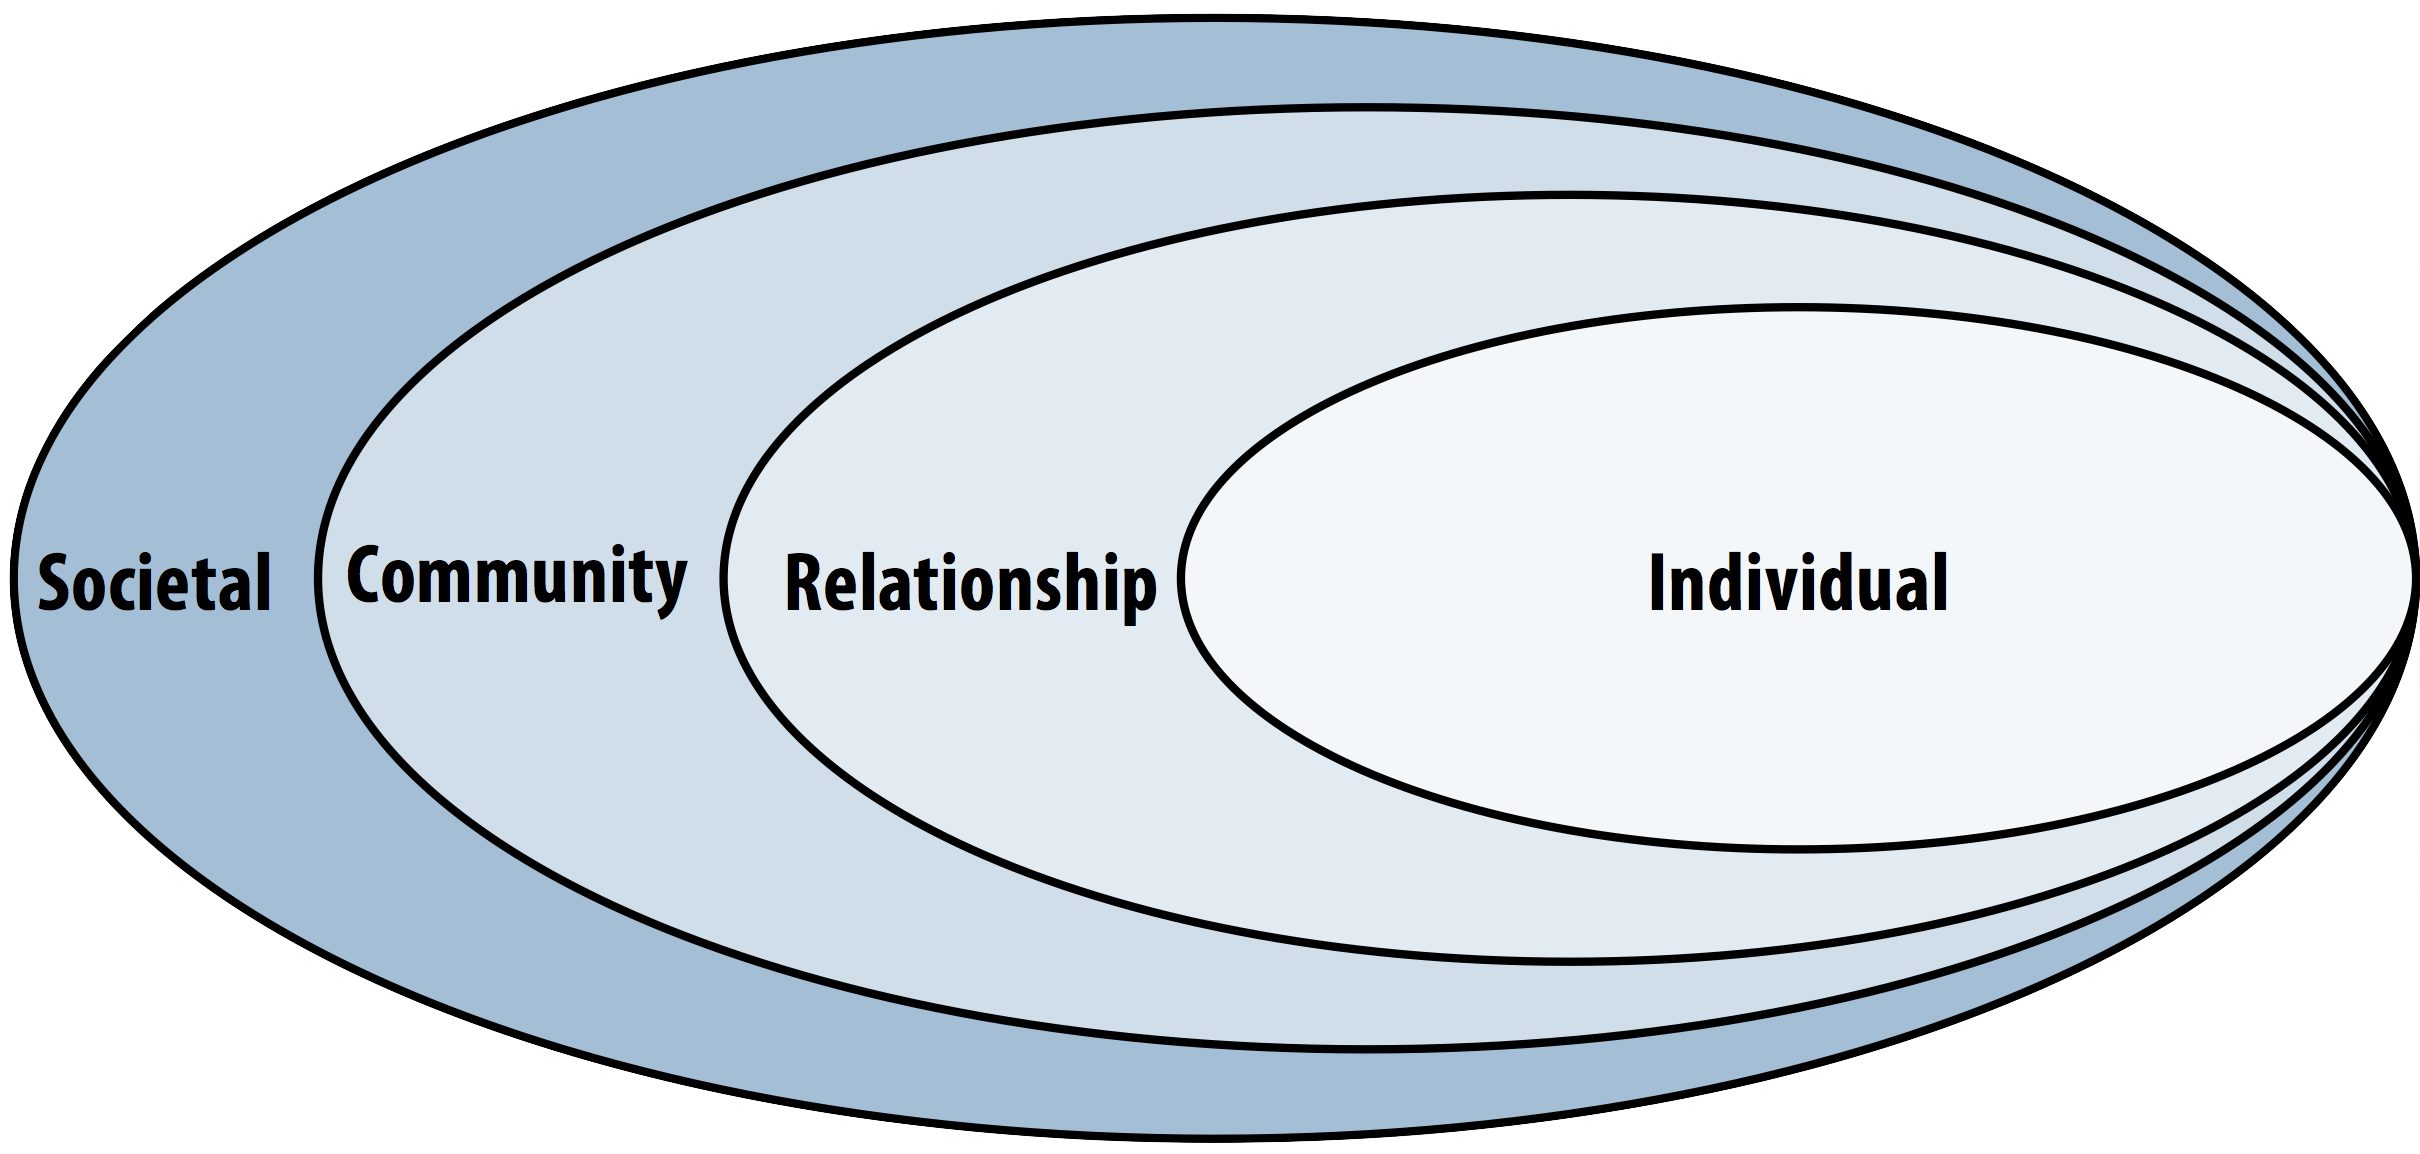
\includegraphics{graphics/inputs/sem.png}
\caption{Social-Ecological Model\label{fig:sem}}
\end{figure}

\newpage

\begin{figure}
\centering
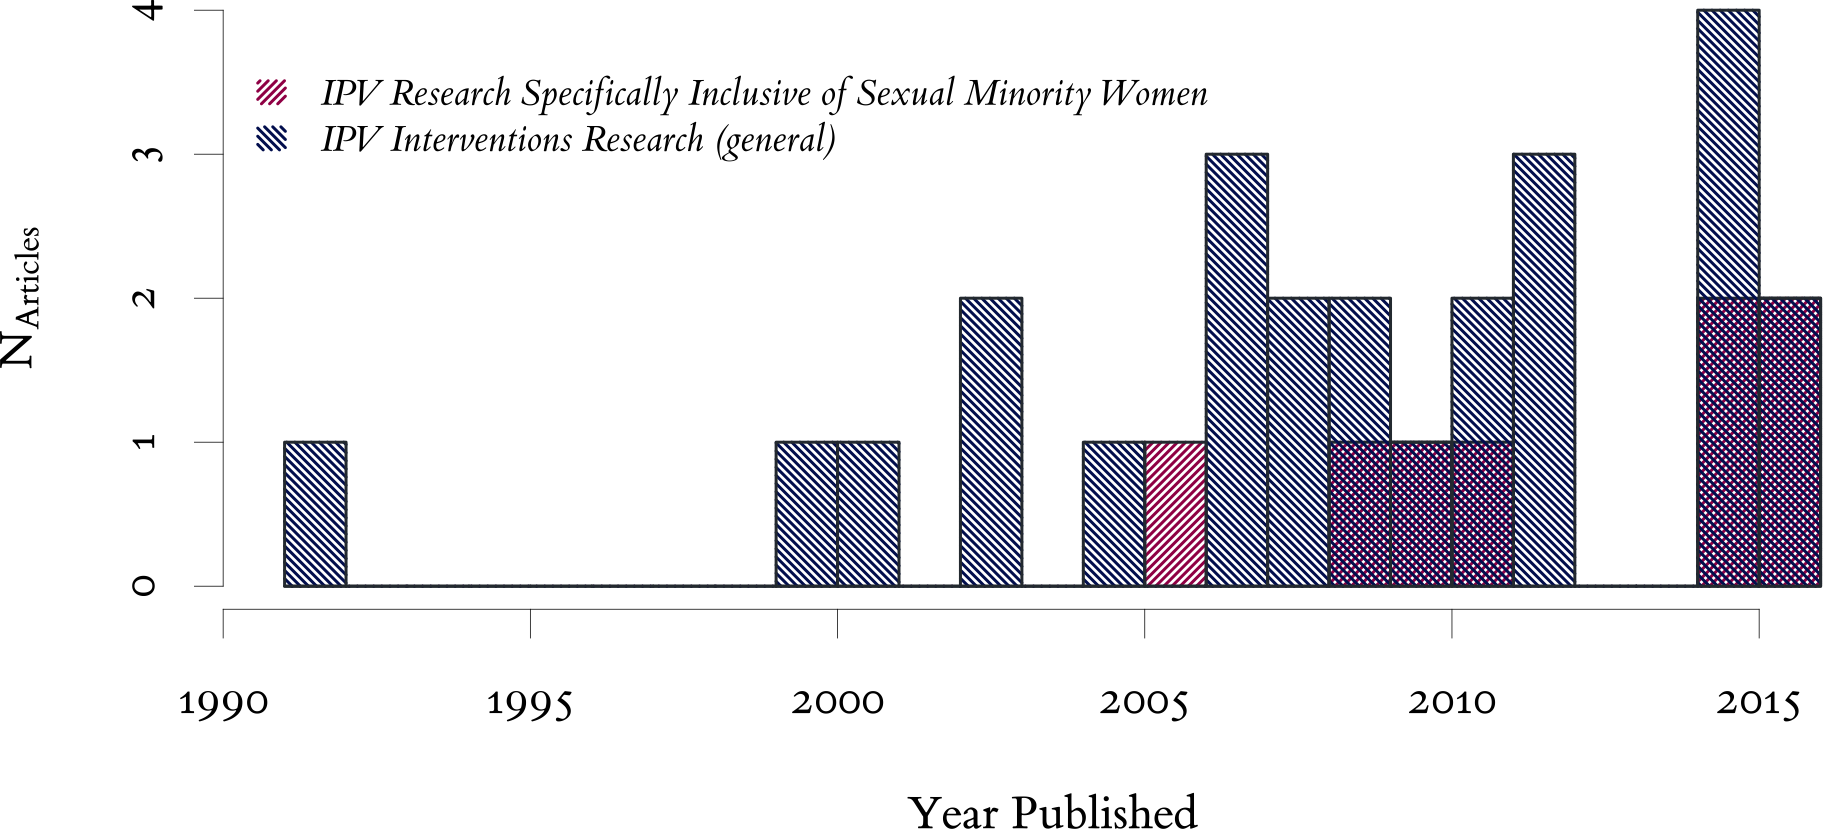
\includegraphics{graphics/inputs/yrhist.png}
\caption{Timeline of publication years of the reviewed
literature\label{fig:yrhist}}
\end{figure}

\newpage

\begin{figure}
\centering
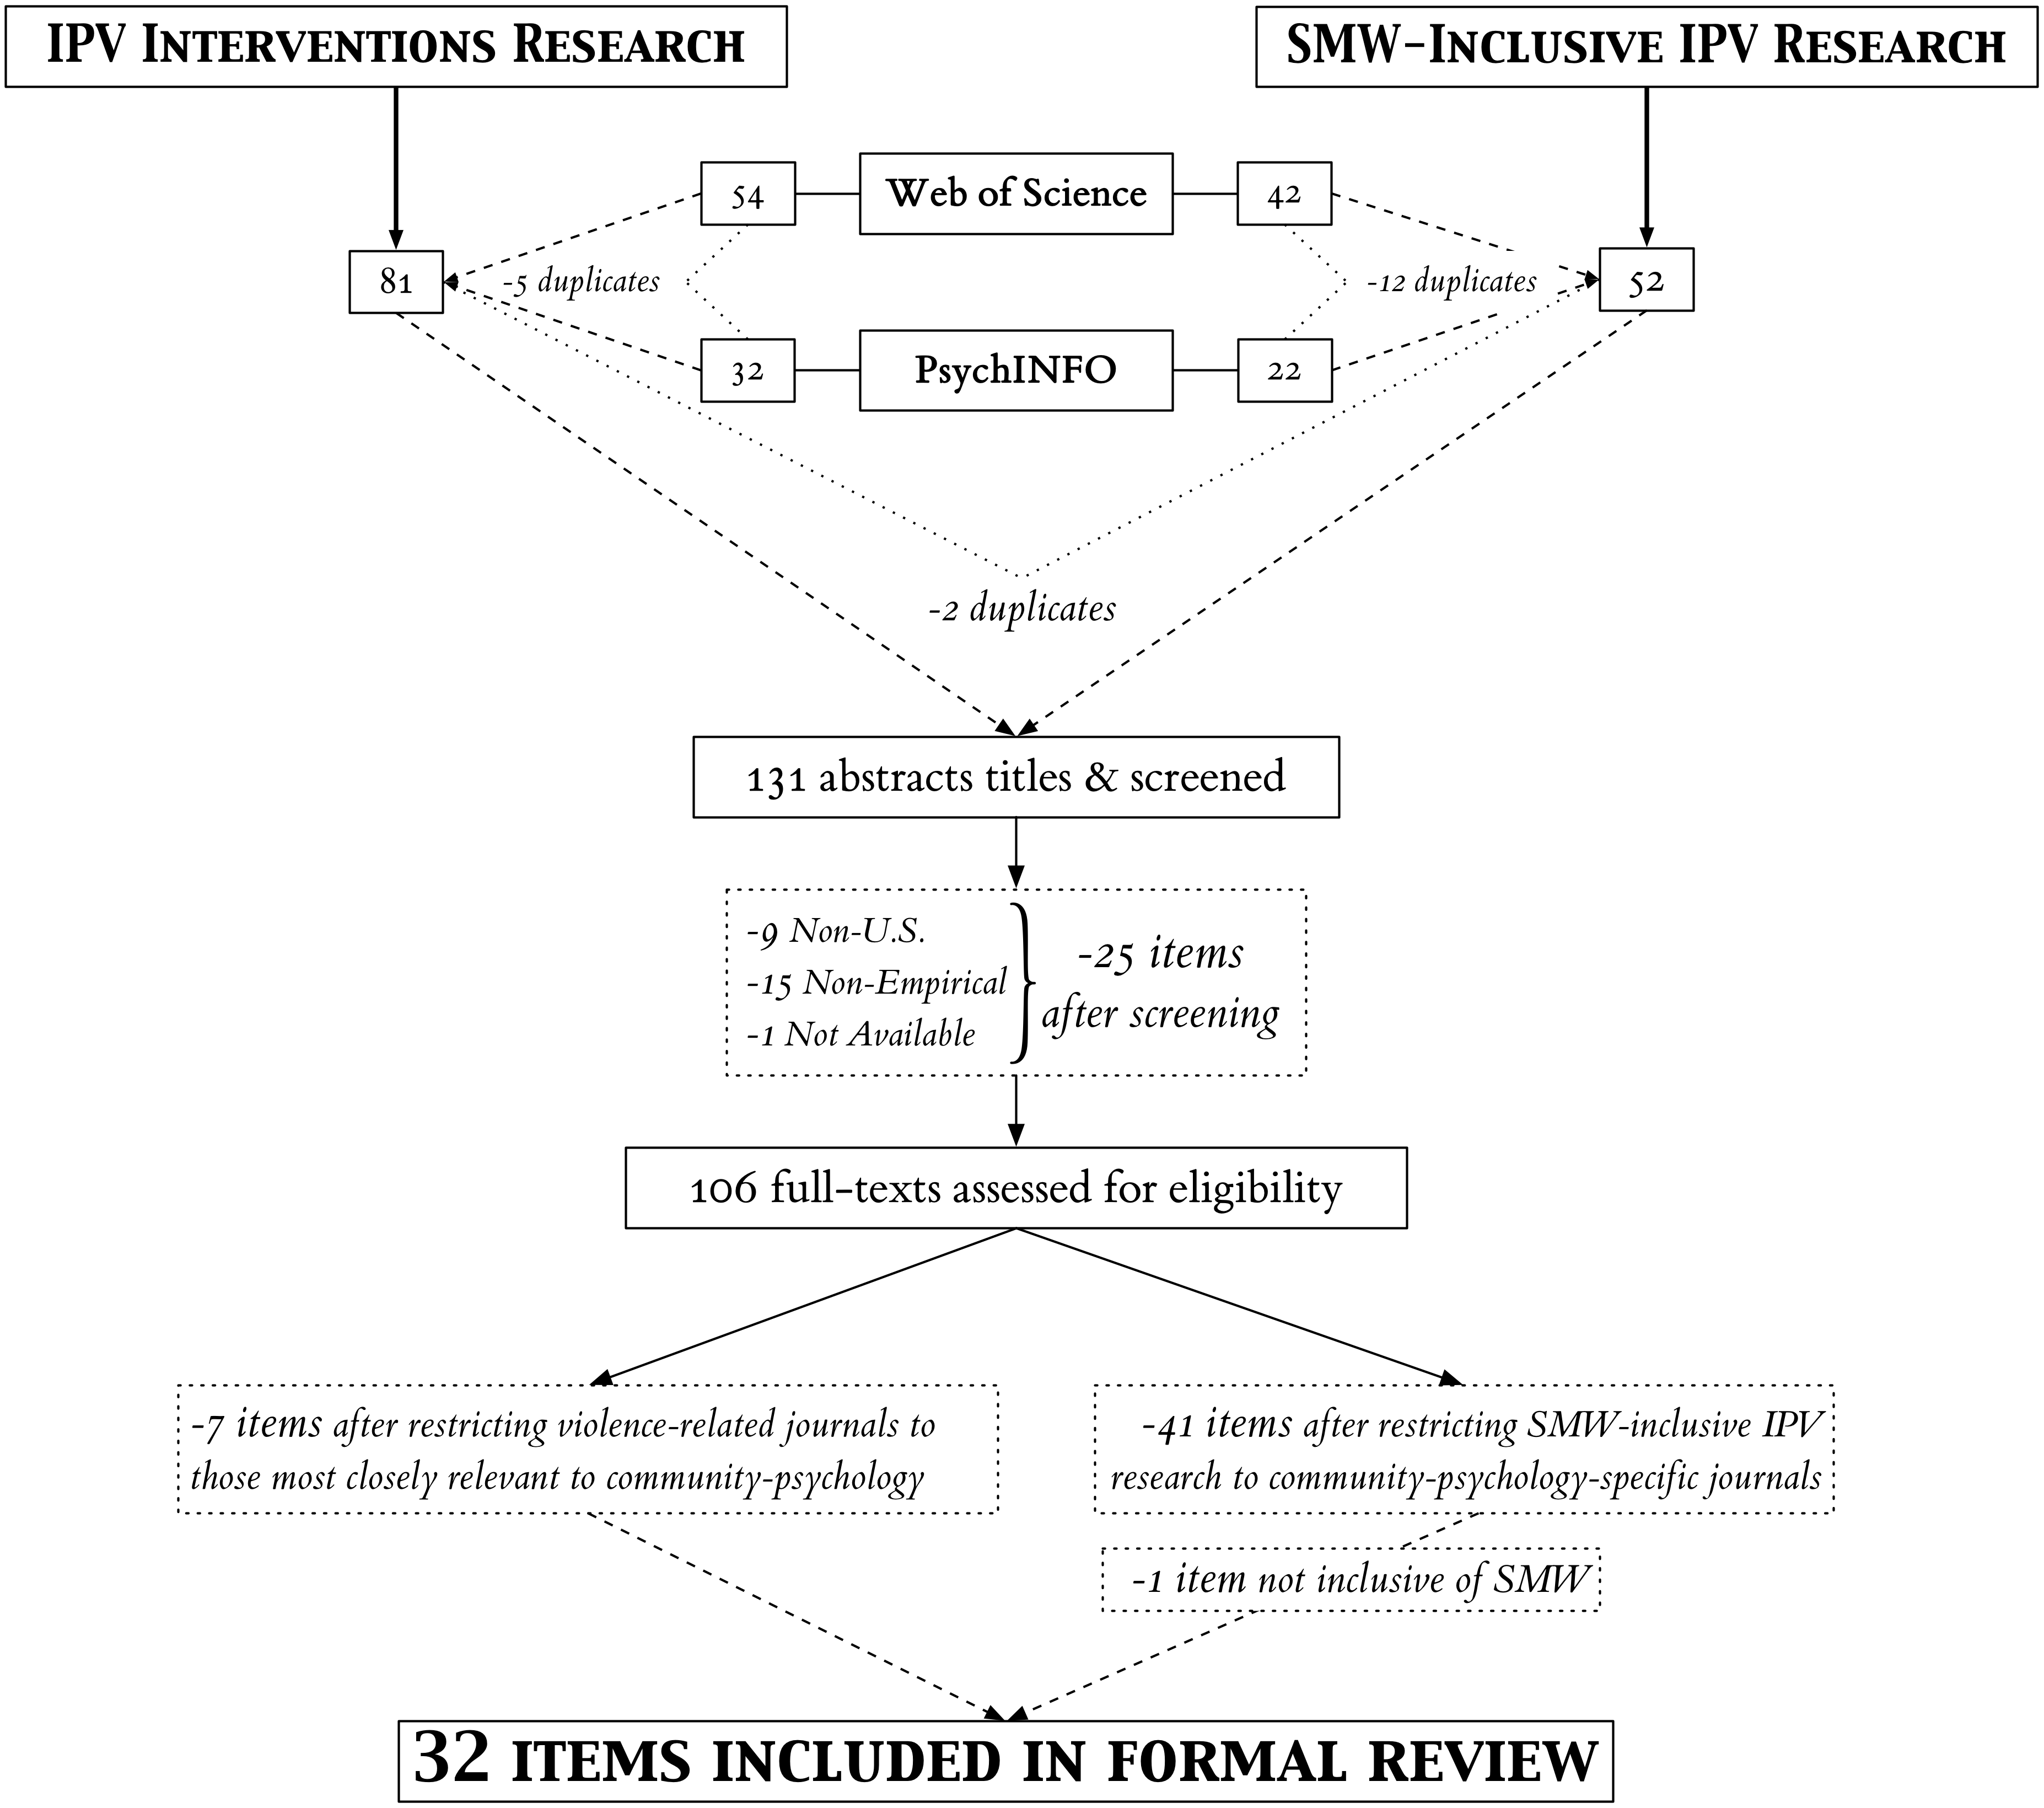
\includegraphics{graphics/inputs/flowchart.png}
\caption{Systematic Literature Search and Inclusion
Flow-Chart\label{fig:flowchart}}
\end{figure}

\newpage

\begin{figure}
\centering
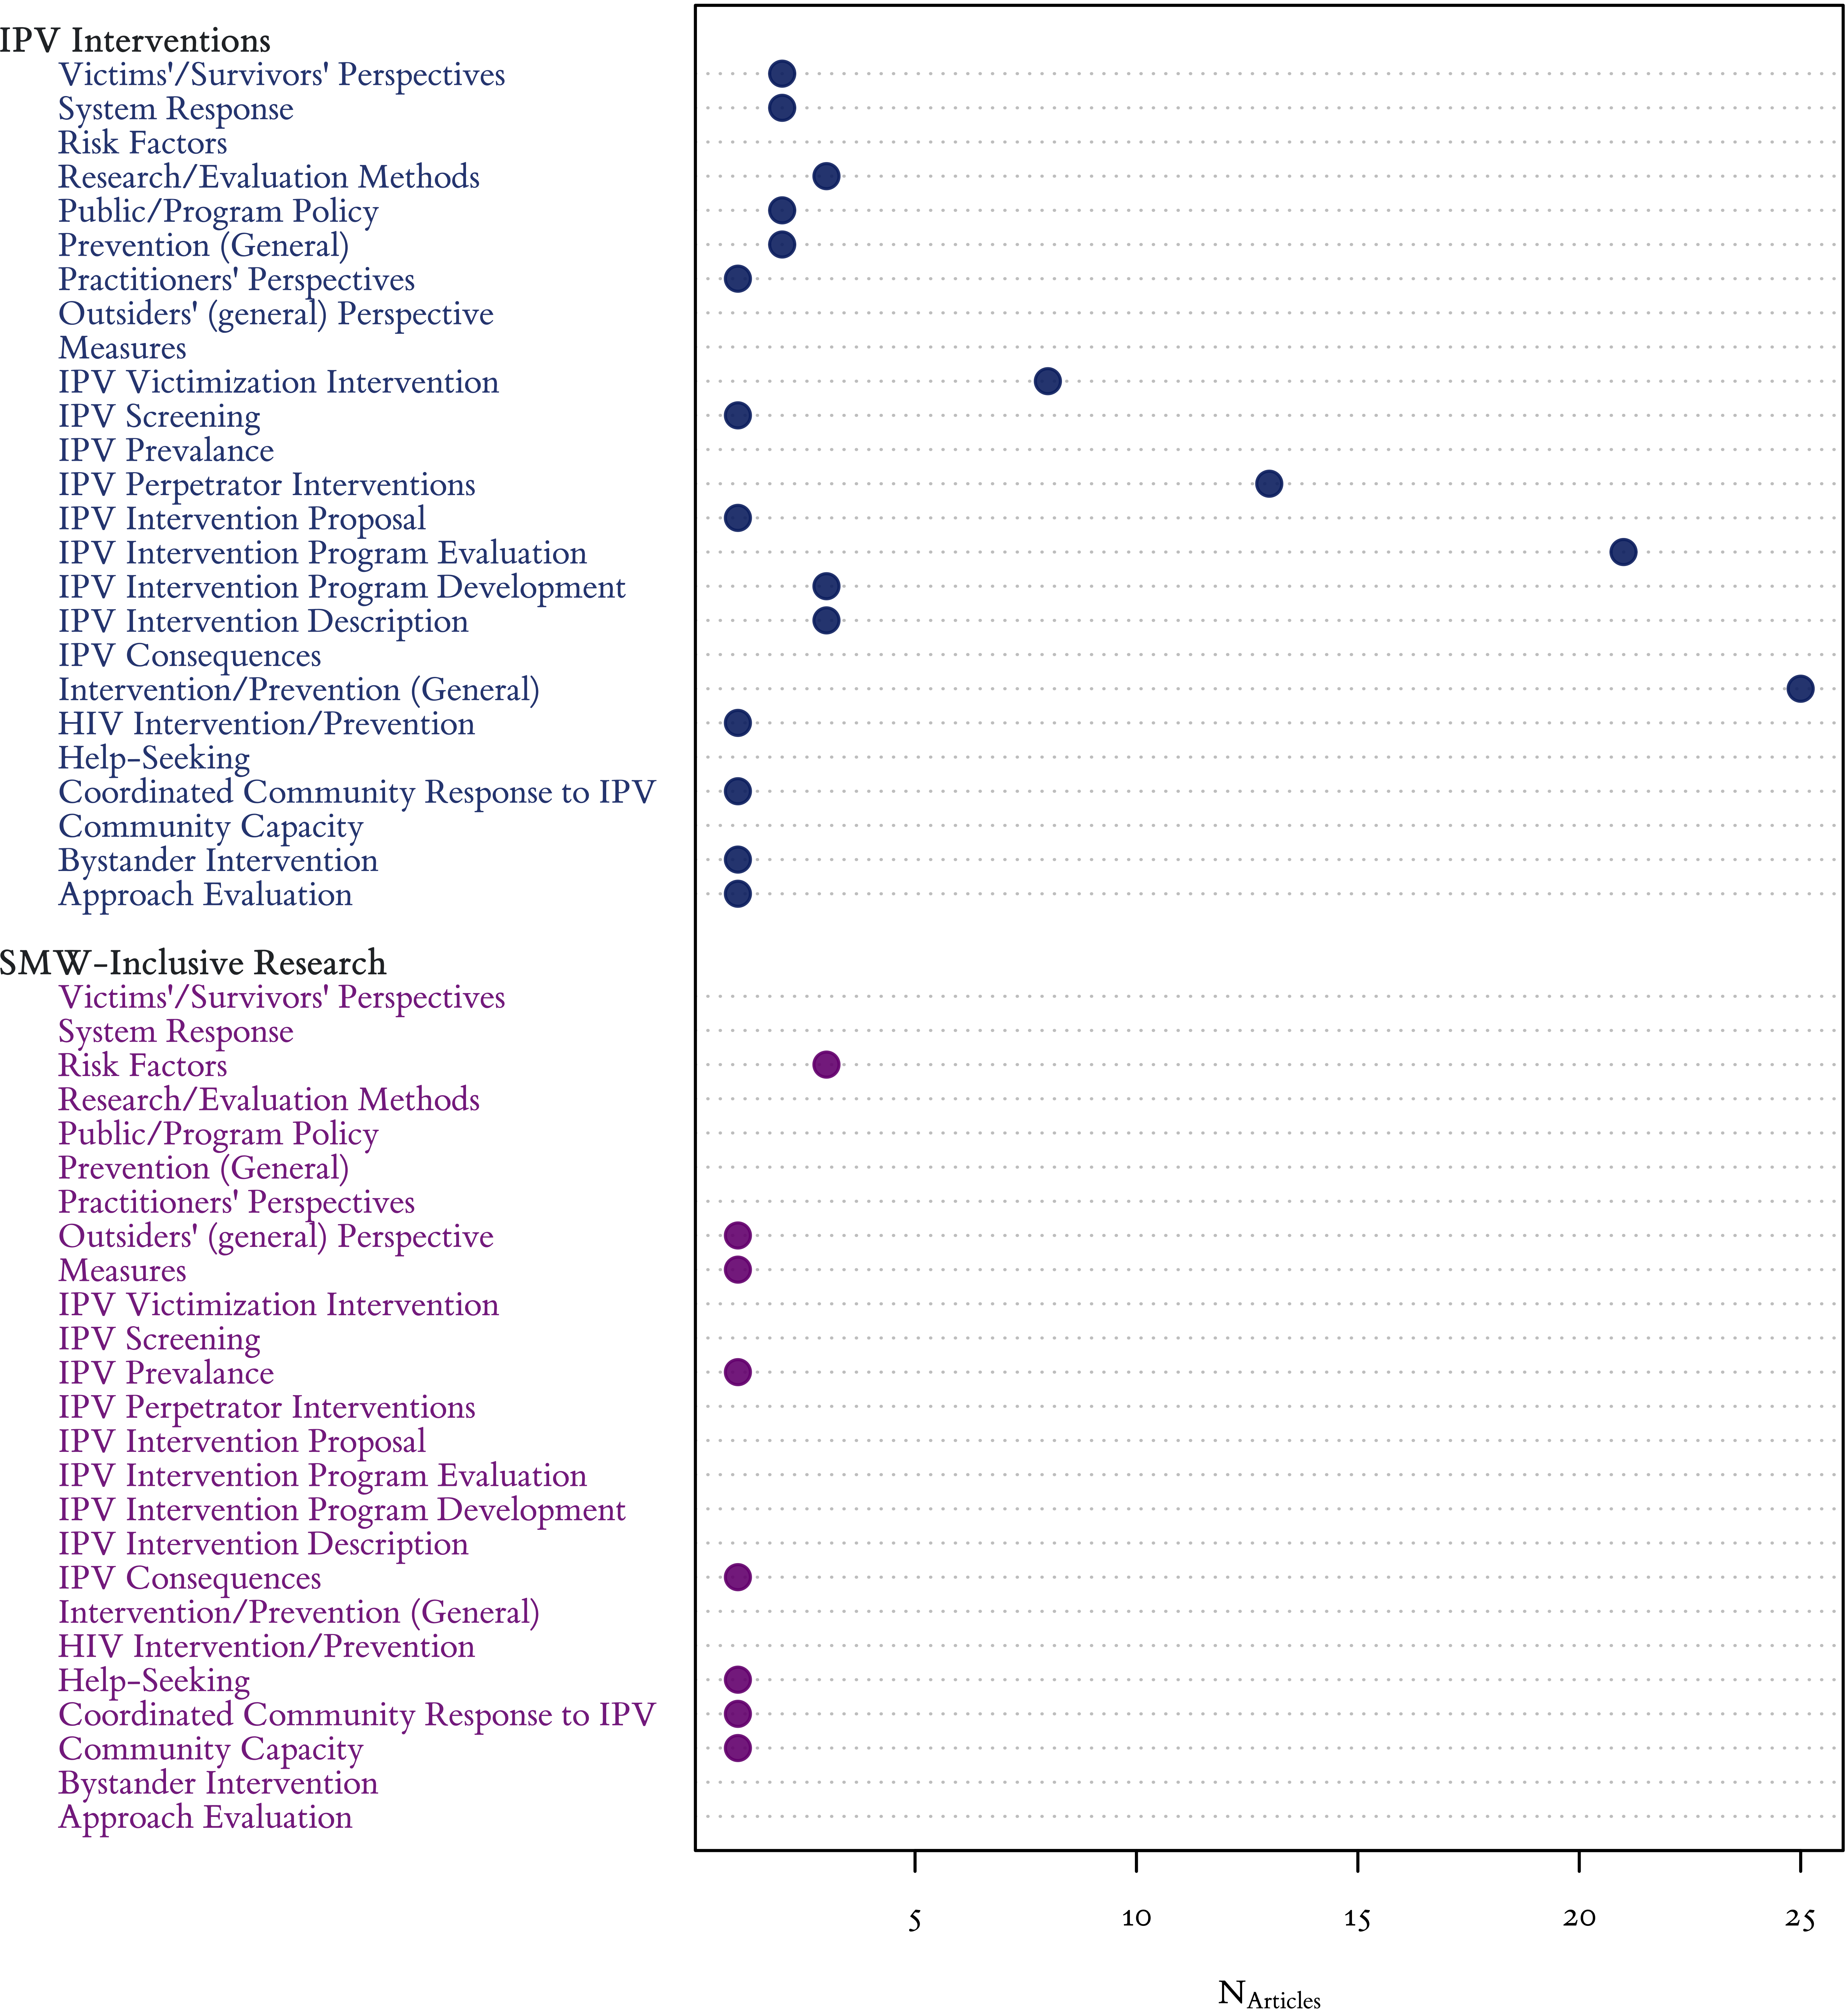
\includegraphics{graphics/inputs/topics.png}
\caption{Substantive Research Topics Covered across the Reviewed
Empirical Research\label{fig:topics}}
\end{figure}

\newpage

\begin{figure}
\centering
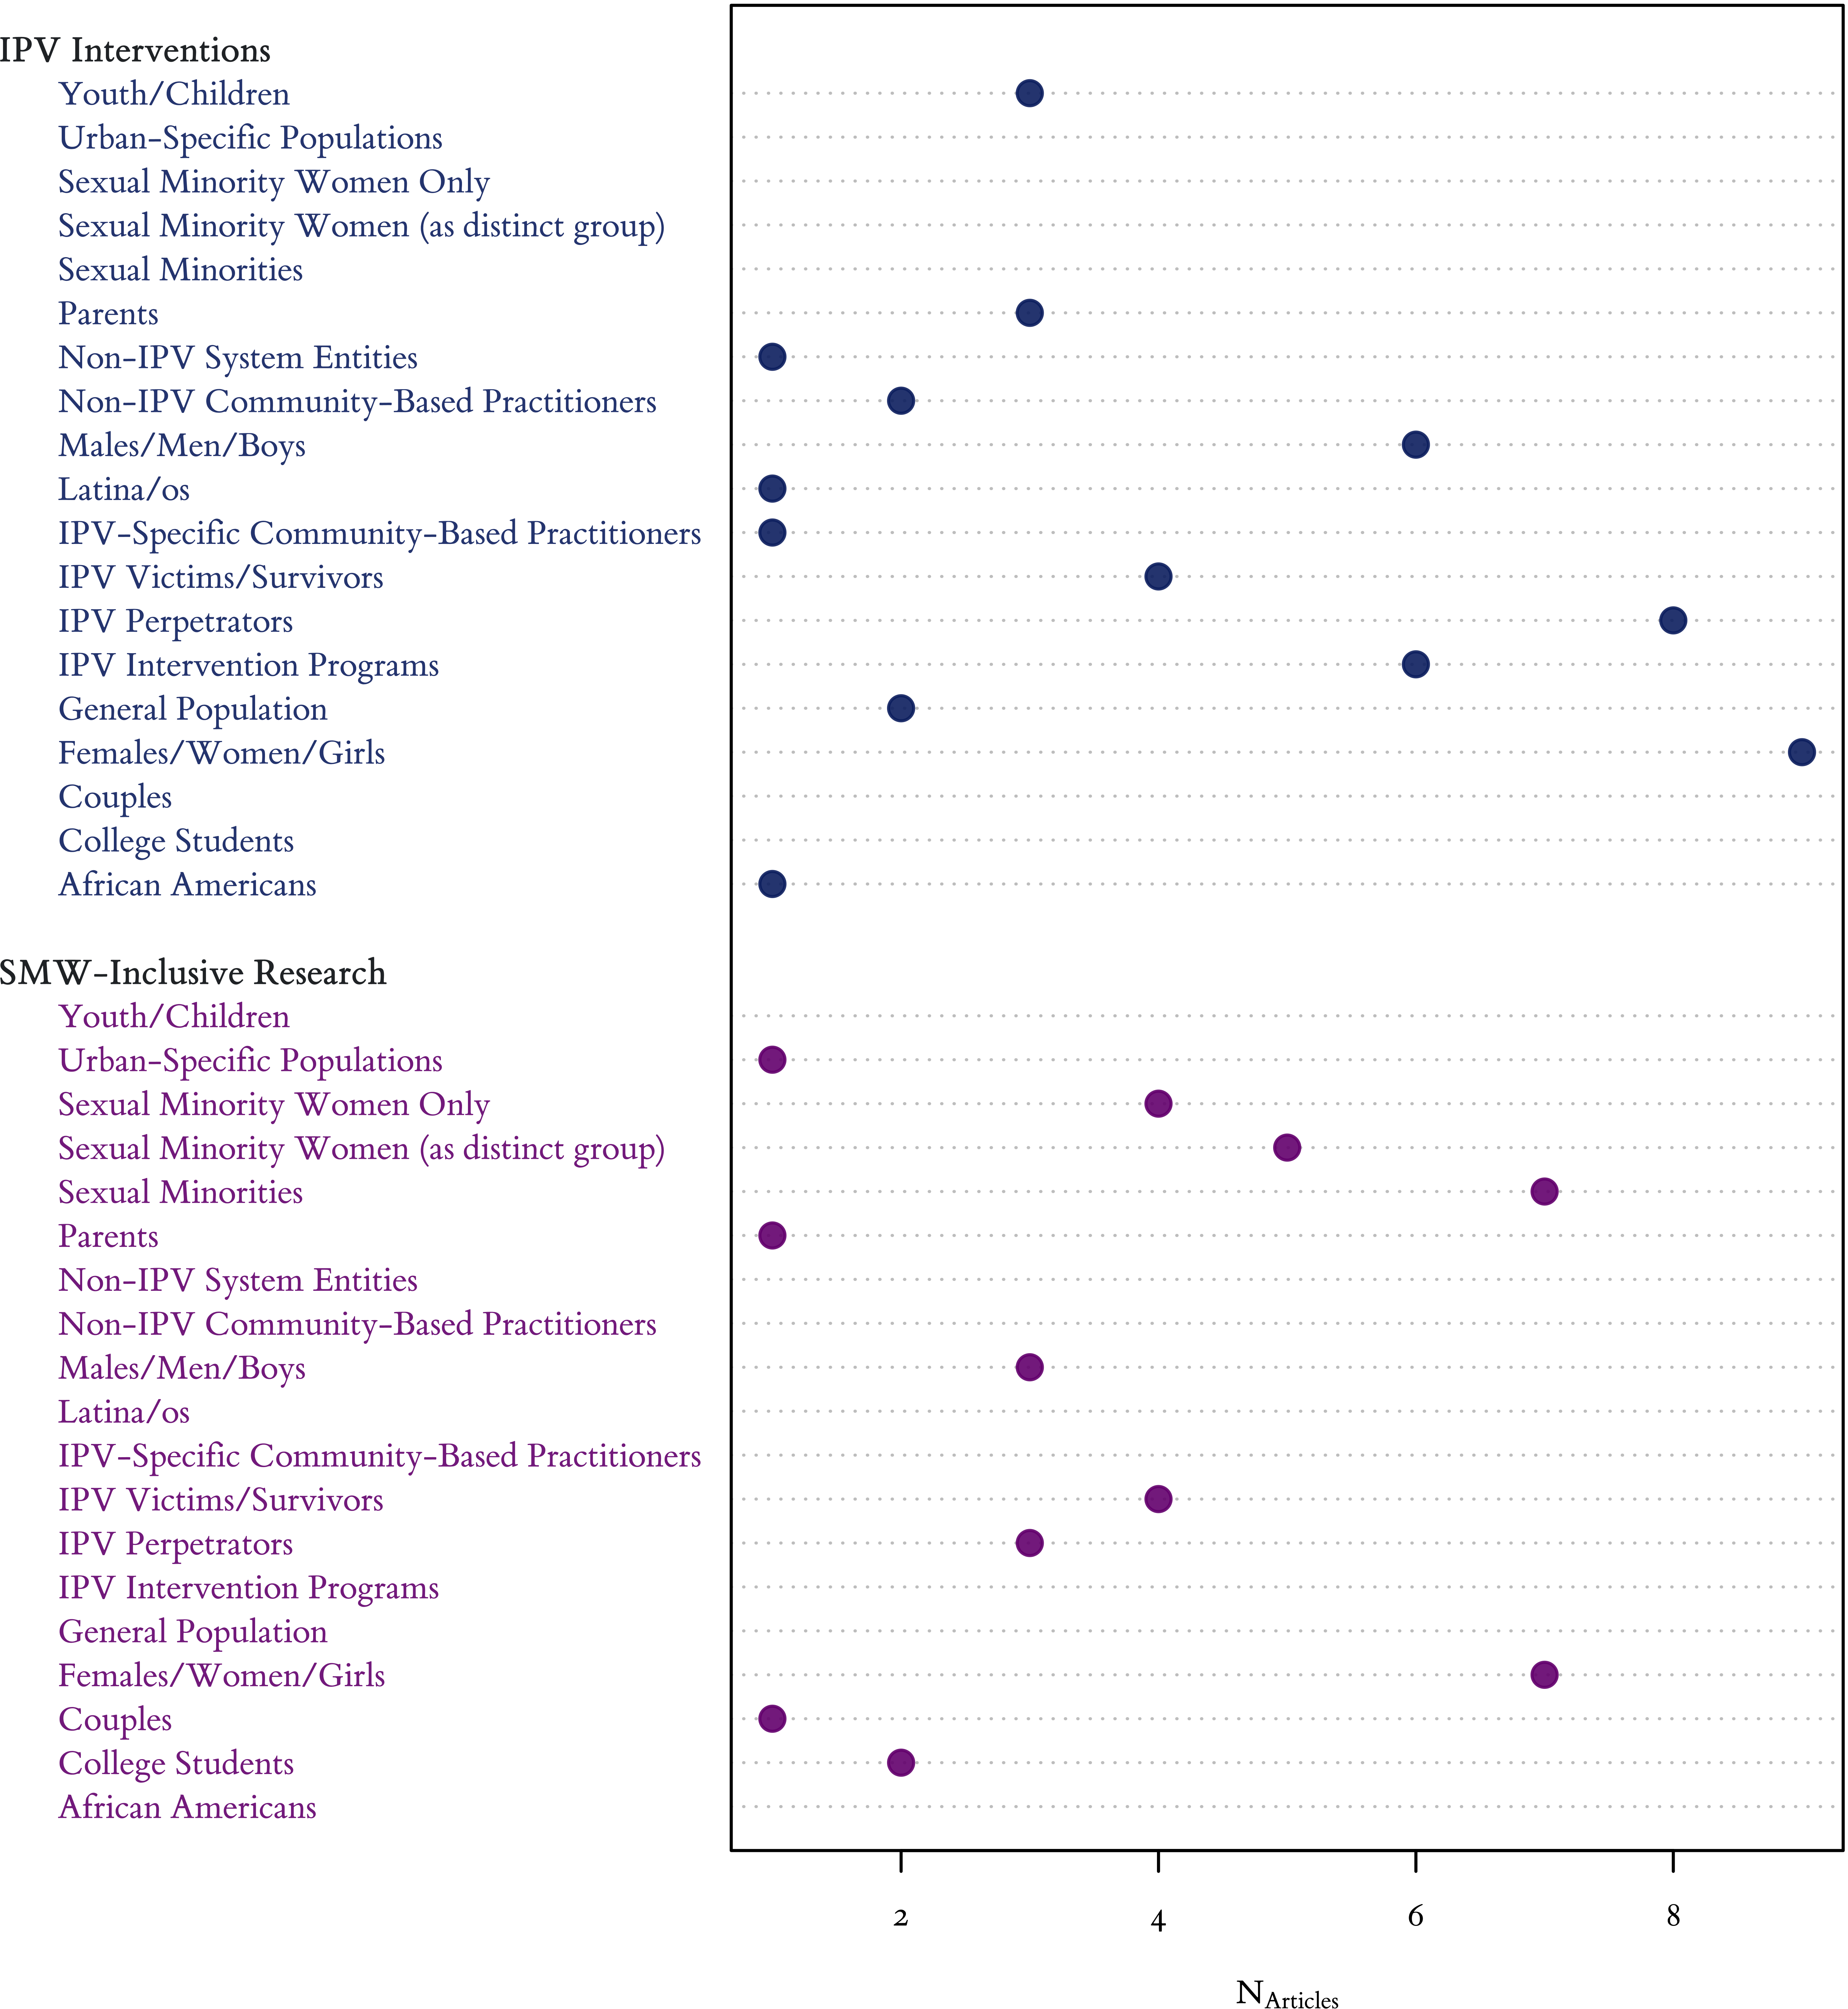
\includegraphics{graphics/inputs/populations.png}
\caption{Target Populations \emph{Included} in the Sampling Frames among
the Review Literature in Each Substantive Research
Category\label{fig:populations}}
\end{figure}

\newpage

\begin{figure}
\centering
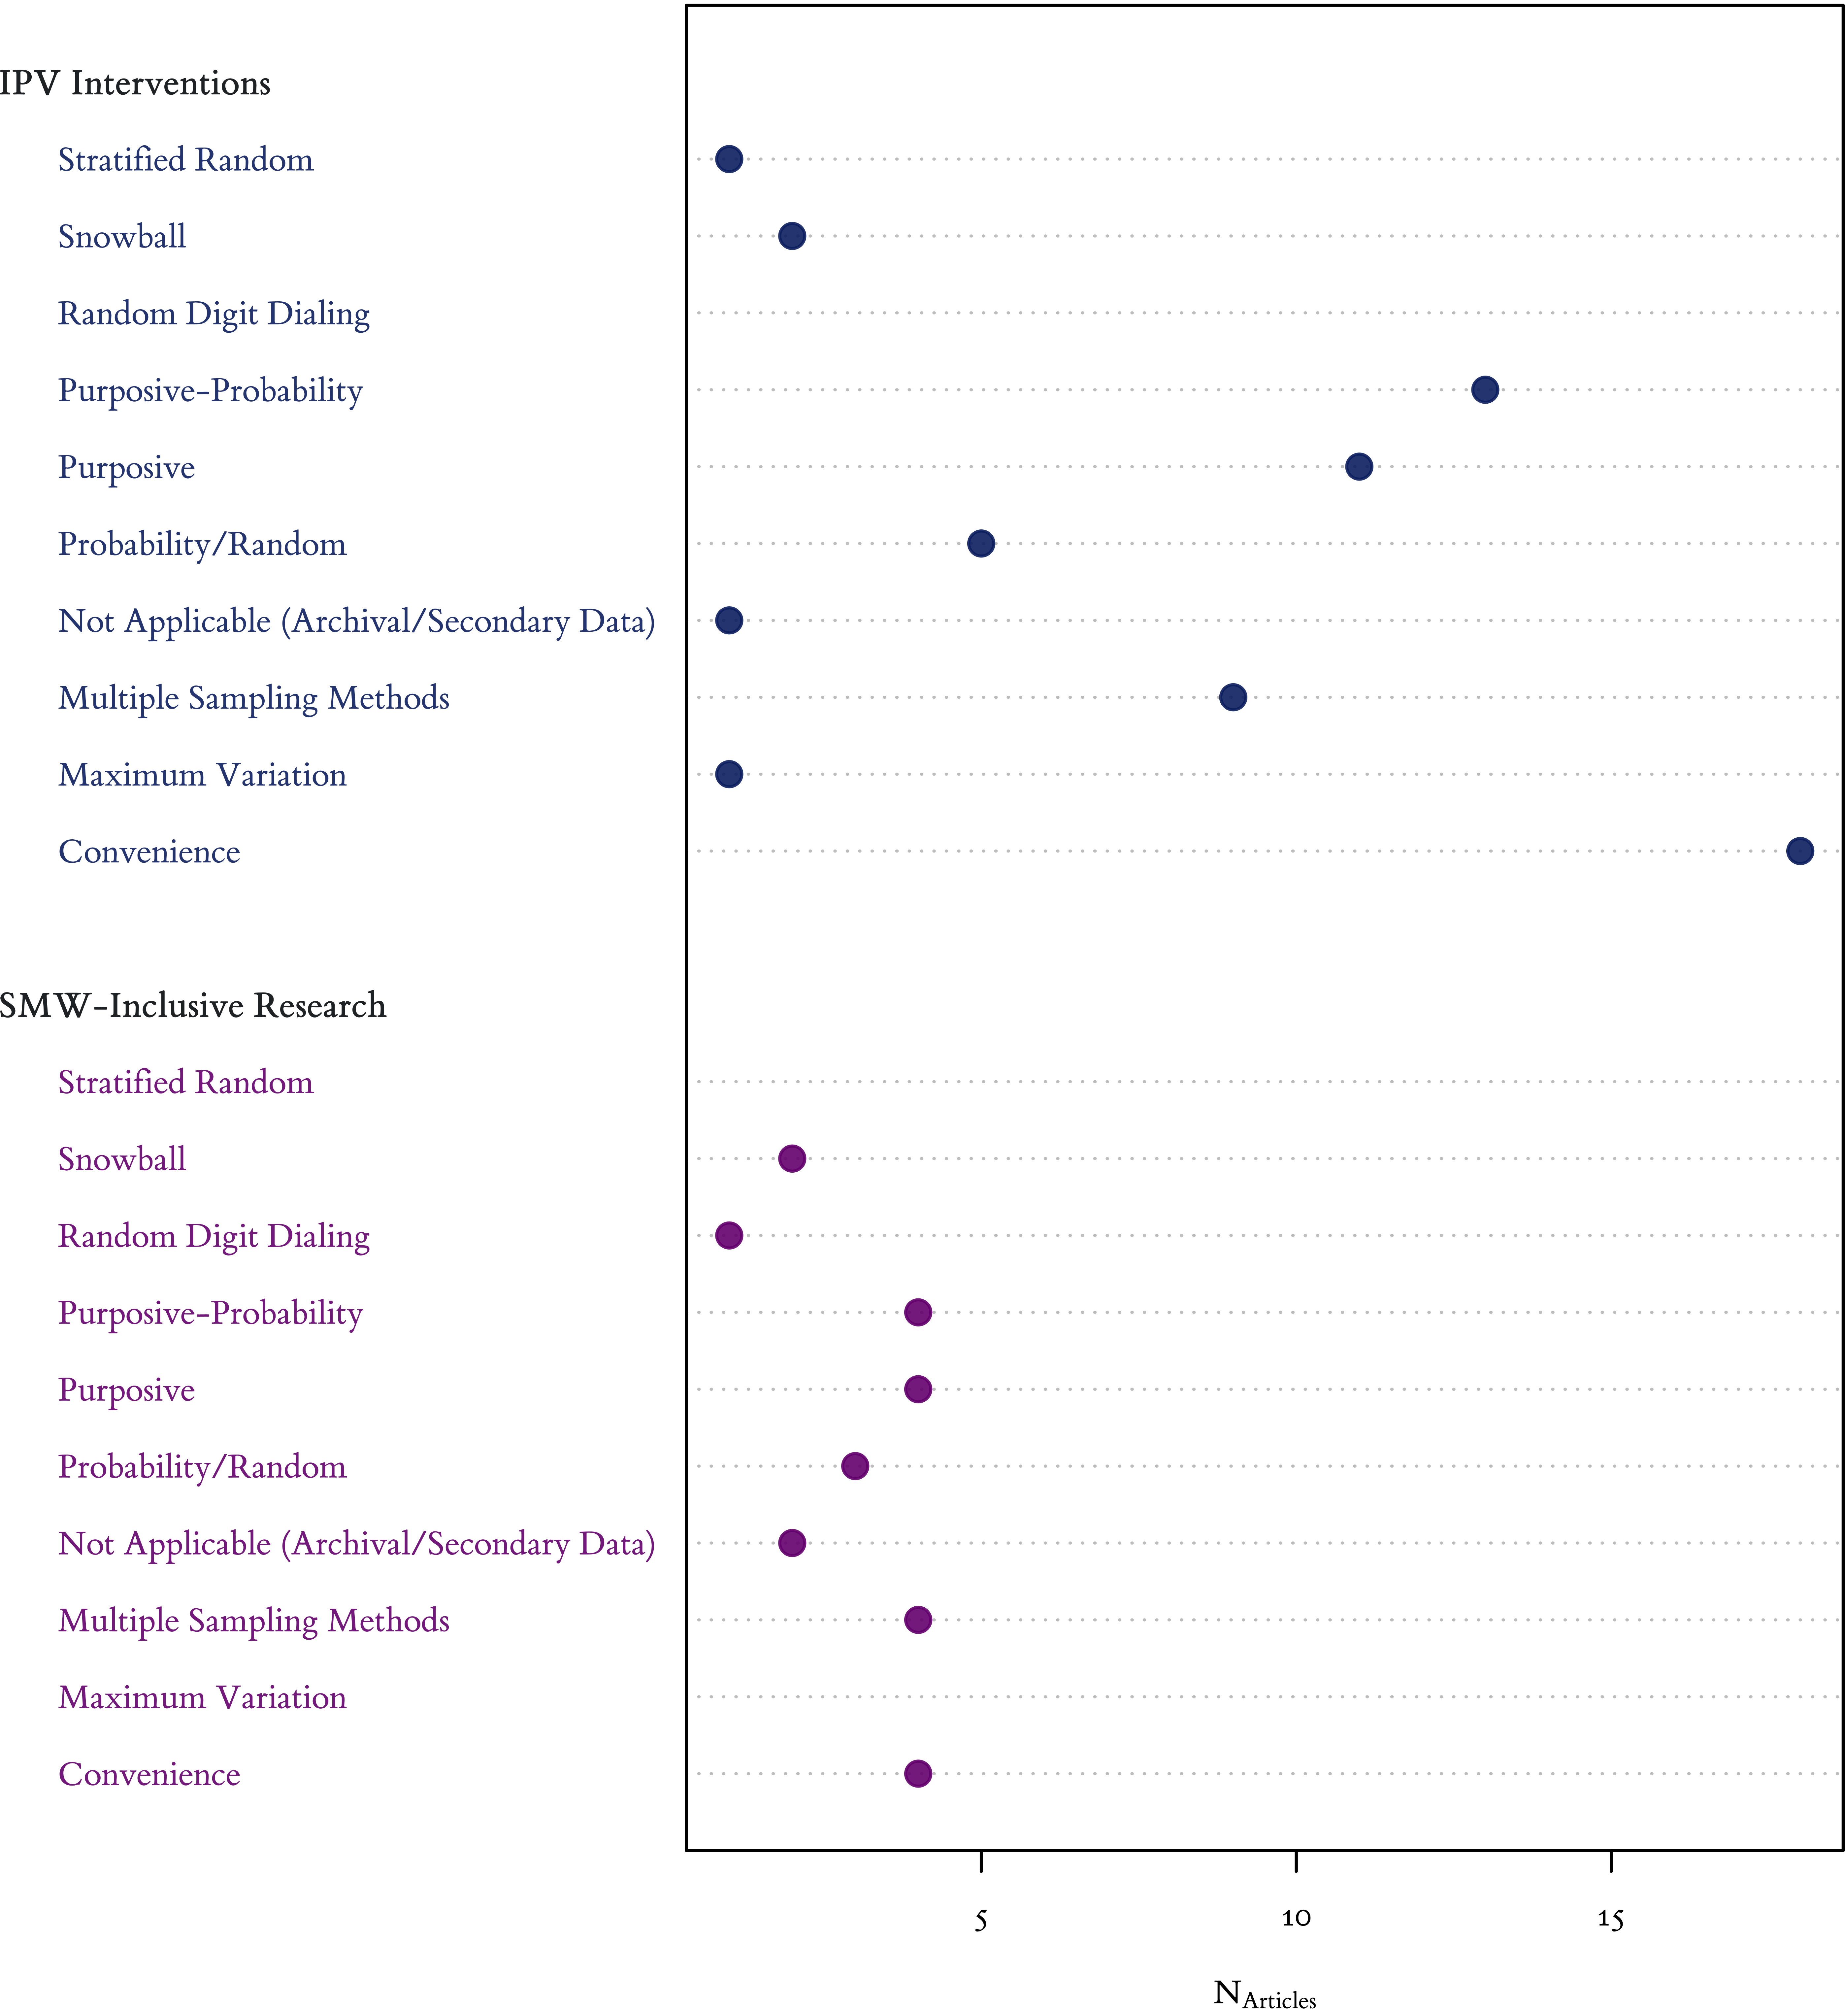
\includegraphics{graphics/inputs/sampling.png}
\caption{Sampling Methods Employed among the Review Literature in Each
Substantive Research Category\label{fig:sampling}}
\end{figure}

\newpage

\begin{figure}
\centering
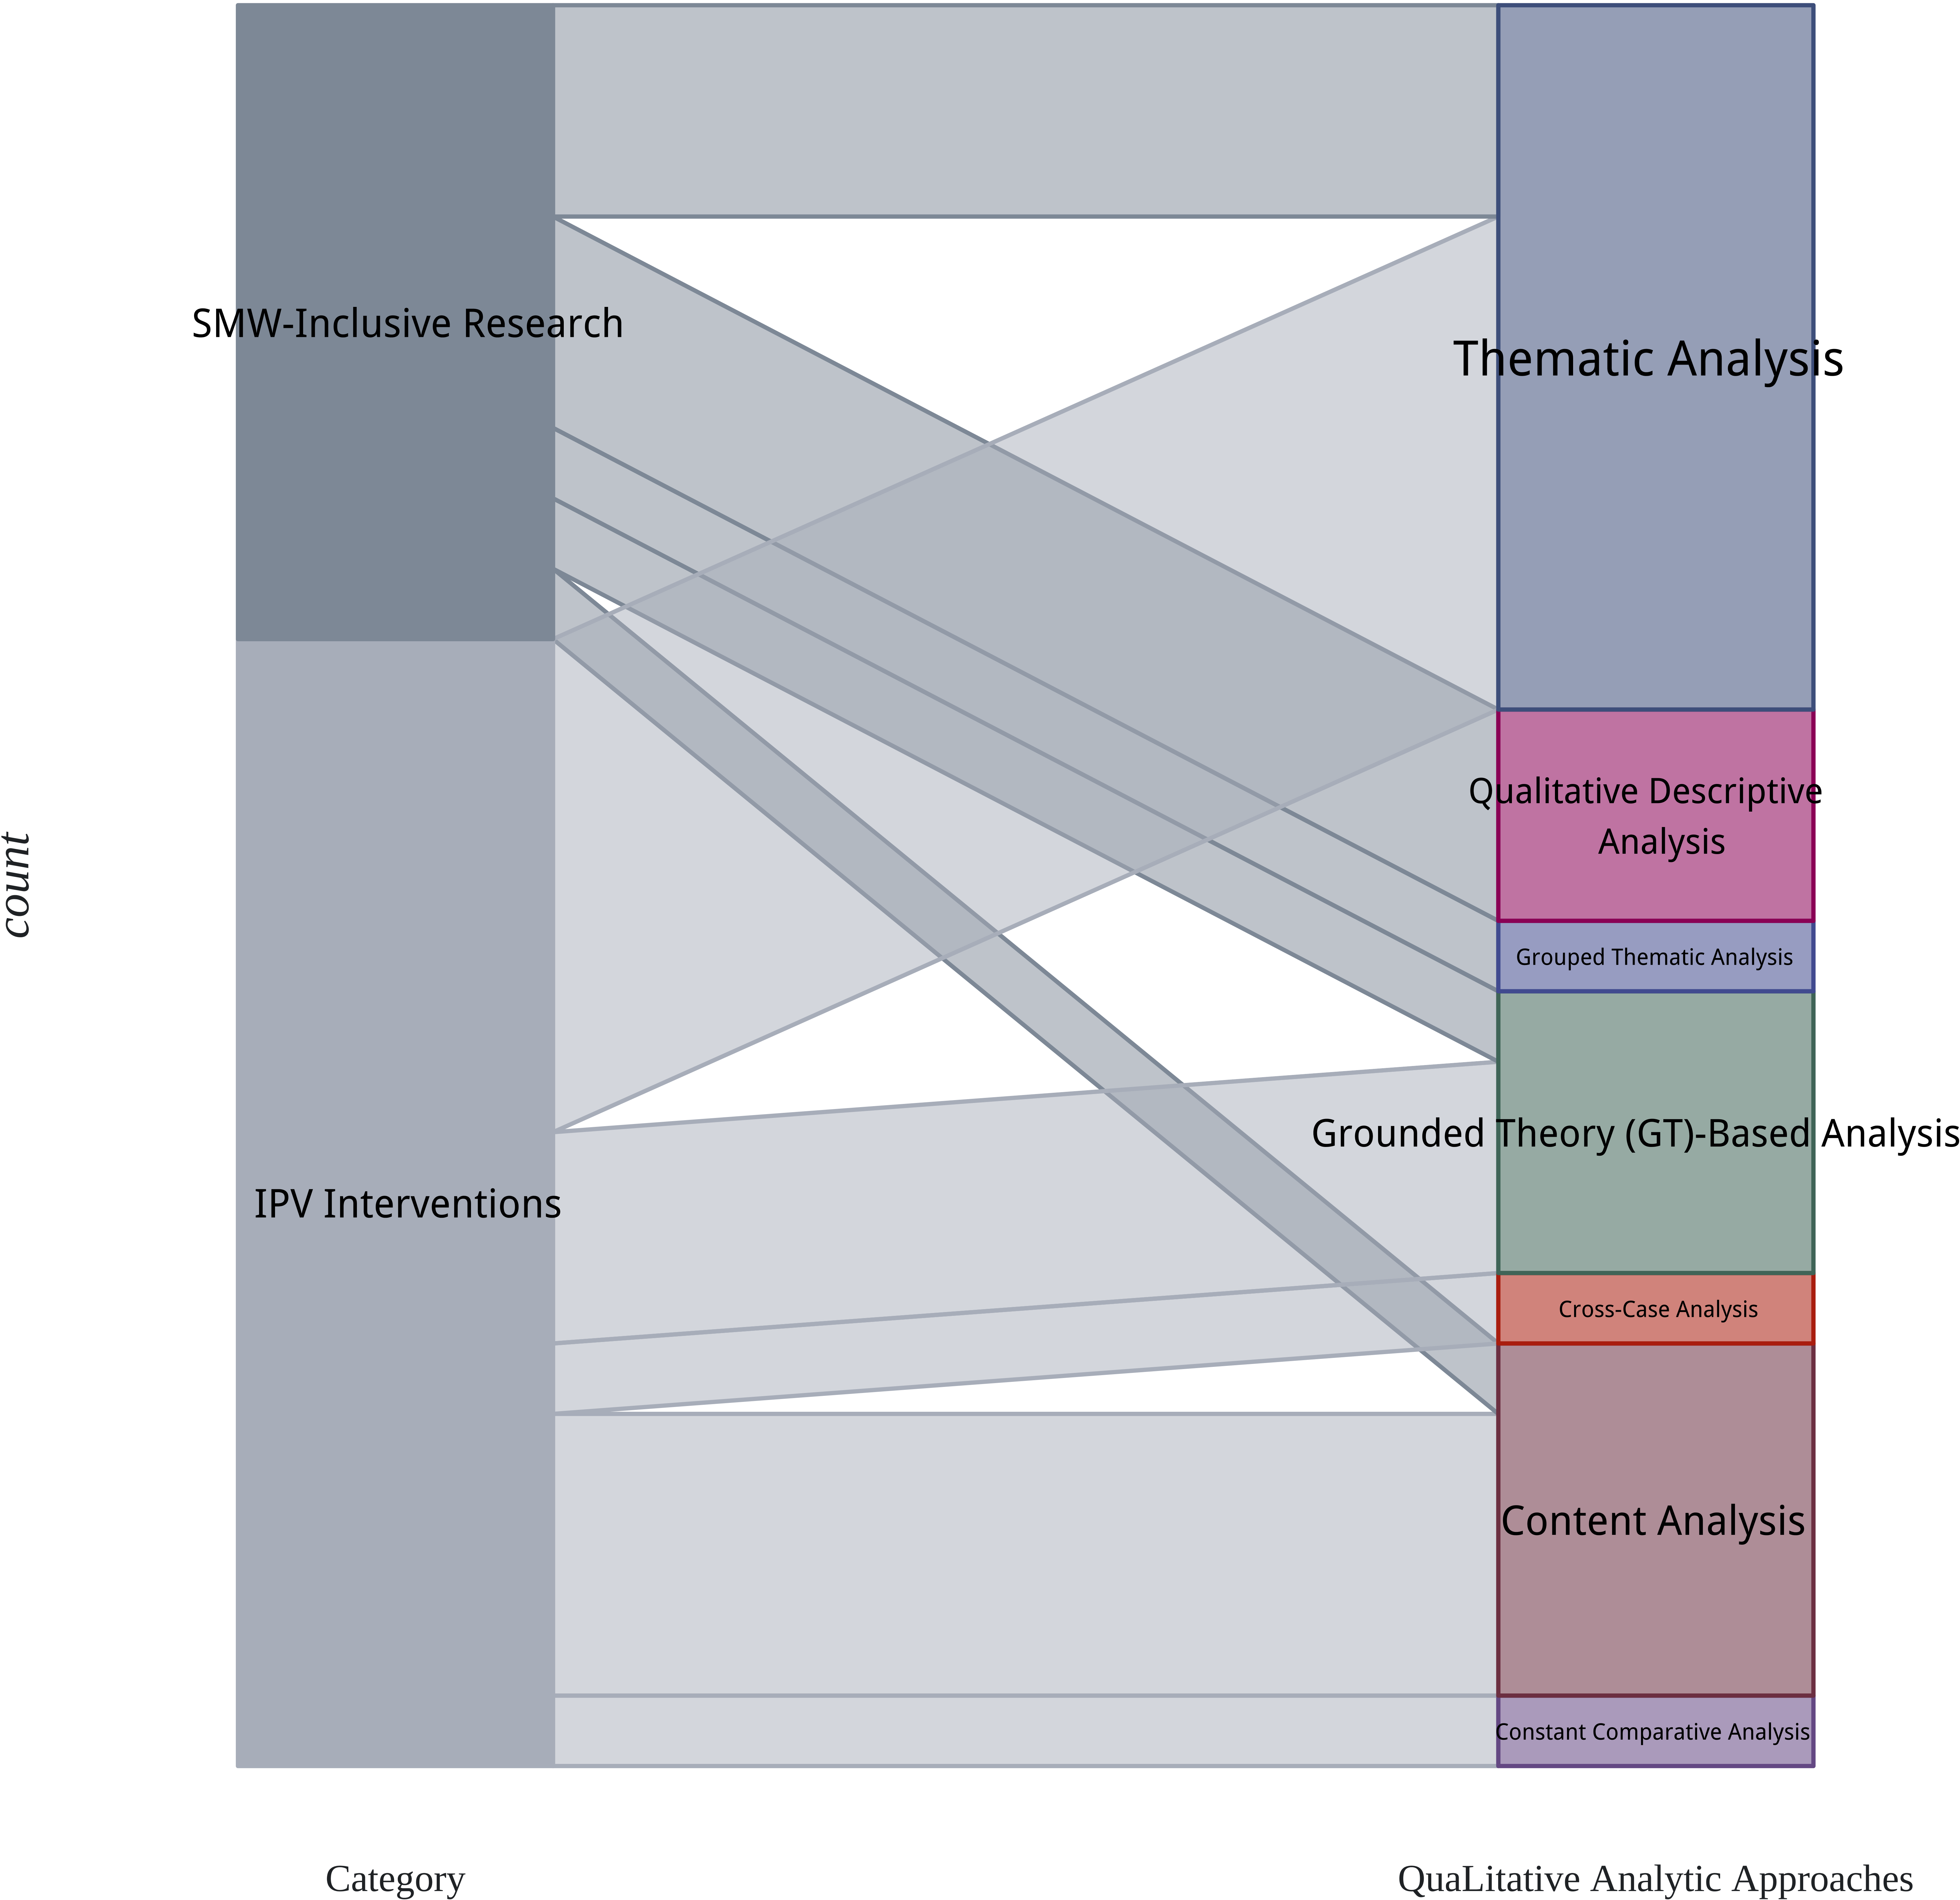
\includegraphics{graphics/inputs/aql.png}
\caption{Qualitative Data Analytic Approaches Implemented among the
Review Literature in Each Substantive Research Category\label{fig:aql}}
\end{figure}

\newpage

\begin{figure}
\centering
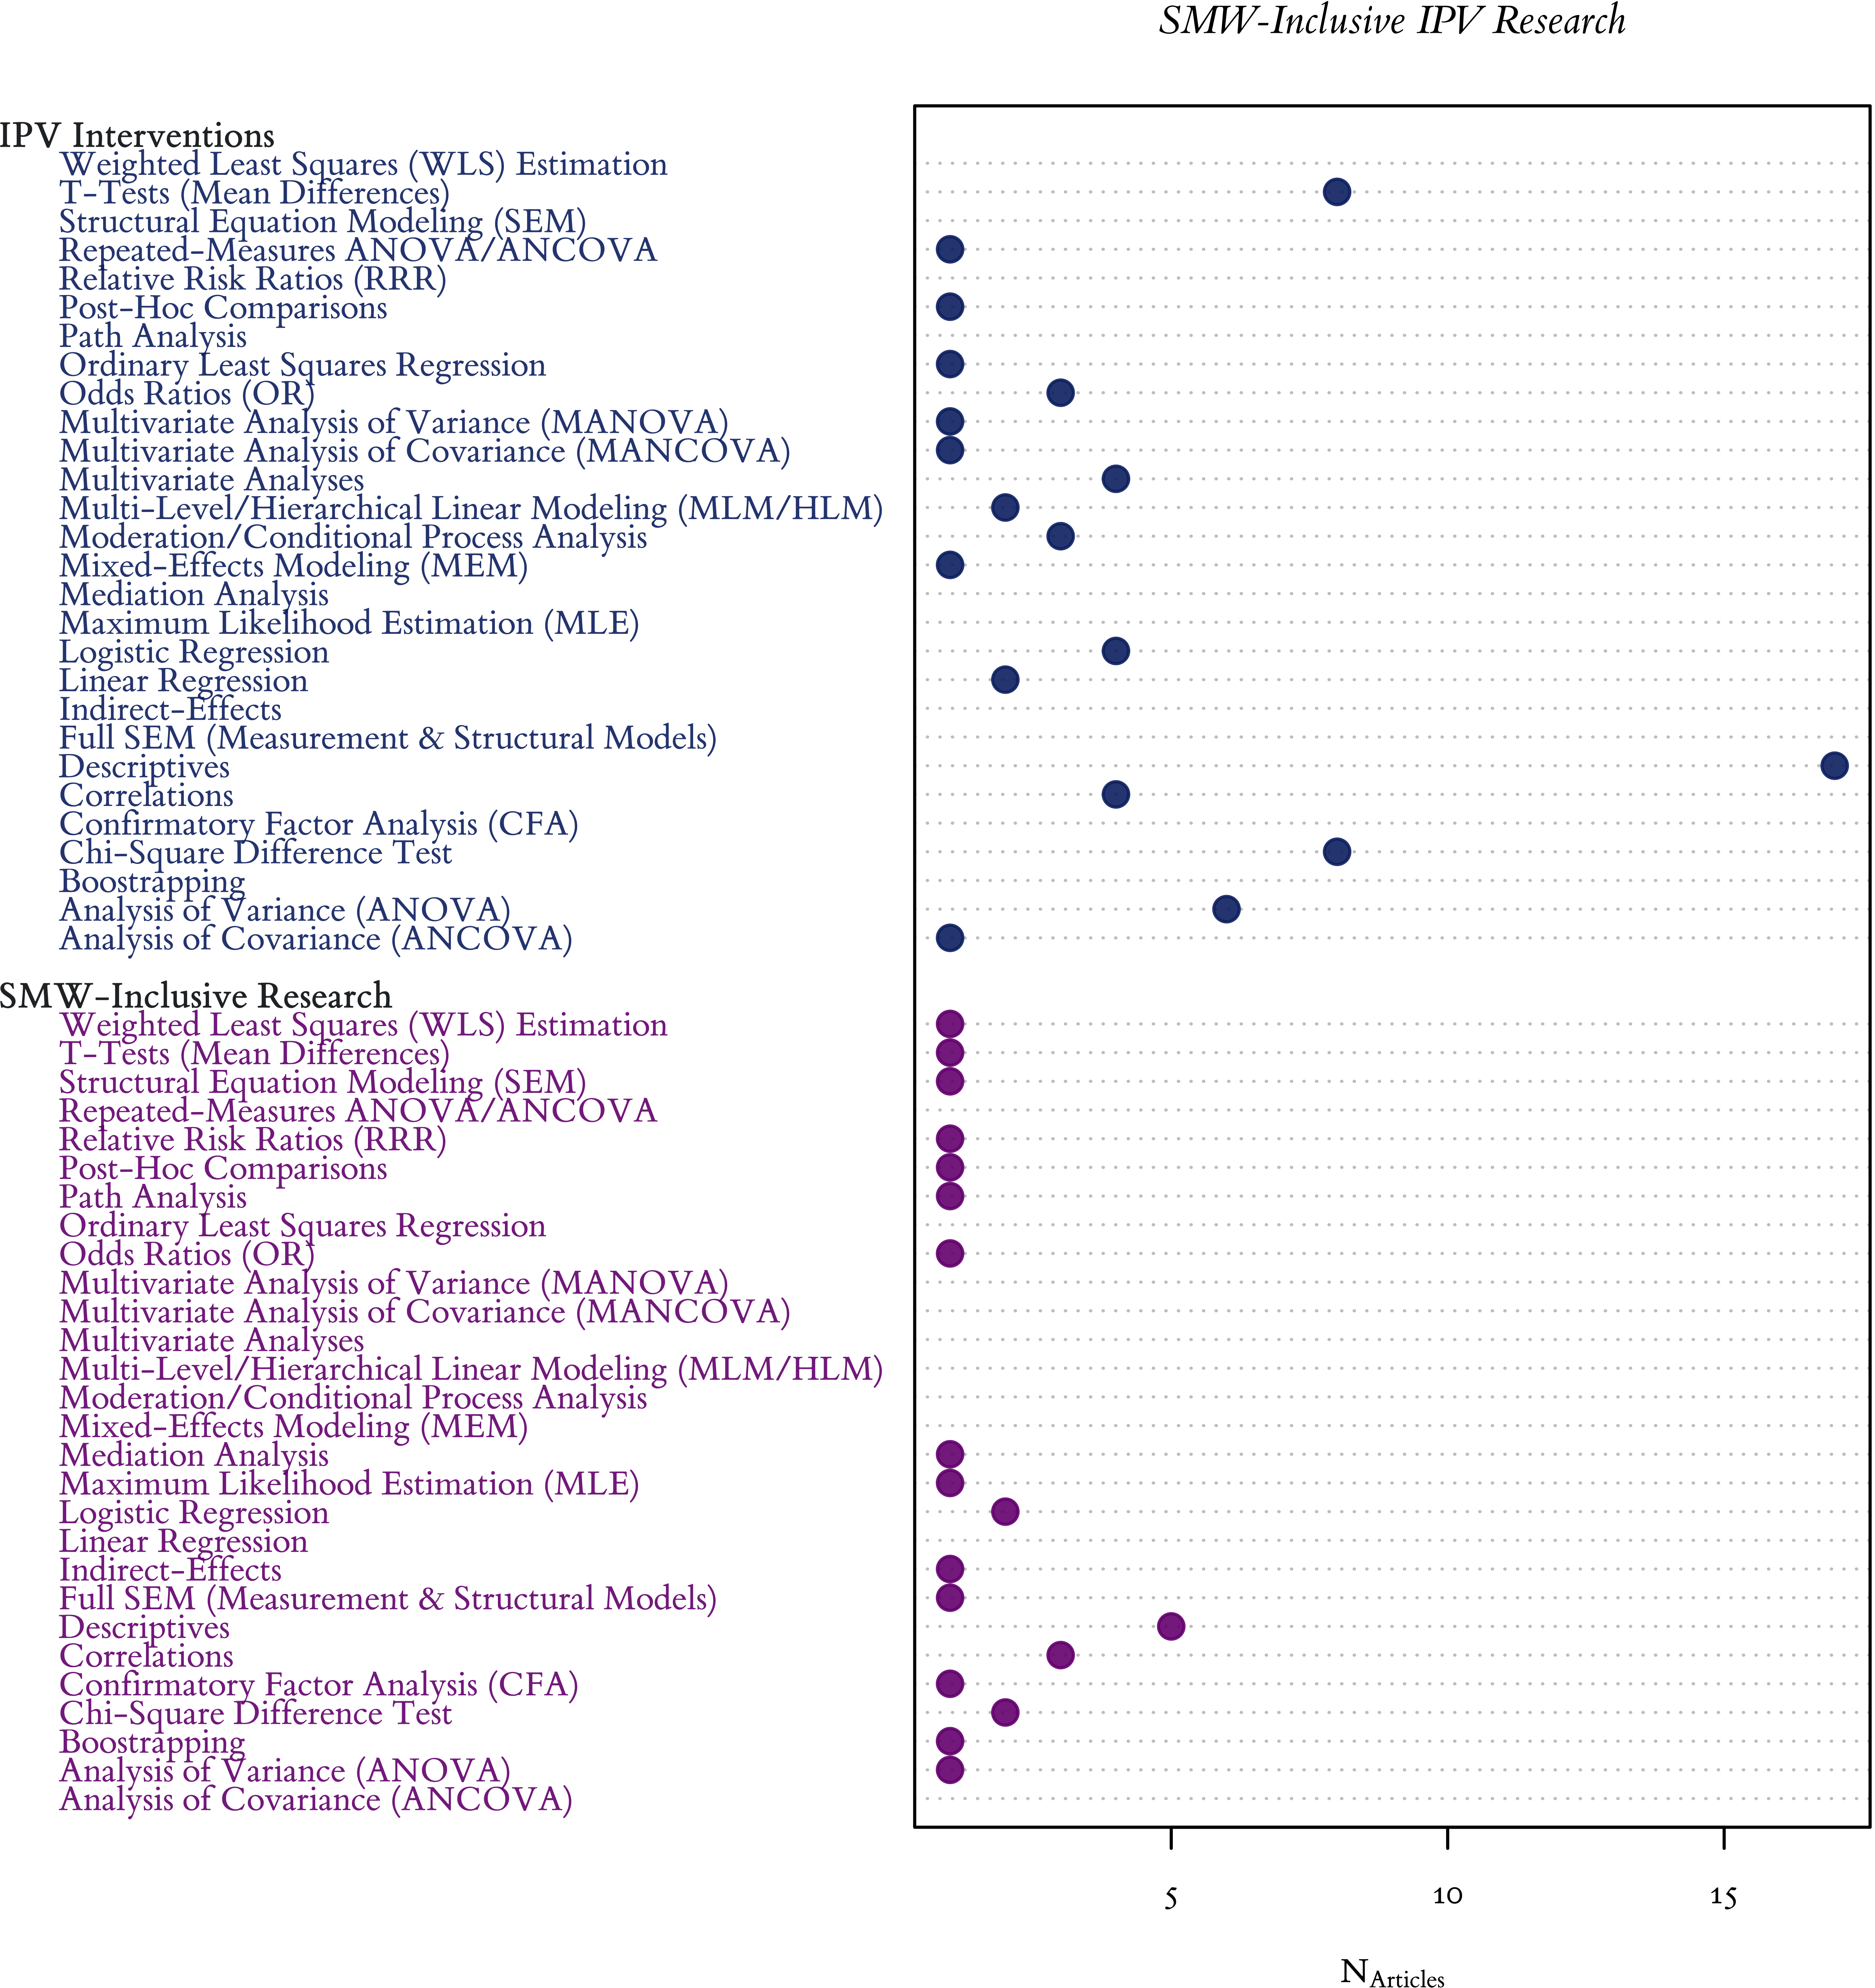
\includegraphics{graphics/inputs/aqt.png}
\caption{Quantitative Data Analytic Approaches Implemented among the
Review Literature in Each Substantive Research Category\label{fig:aqt}}
\end{figure}

\newpage

\begin{figure}
\centering
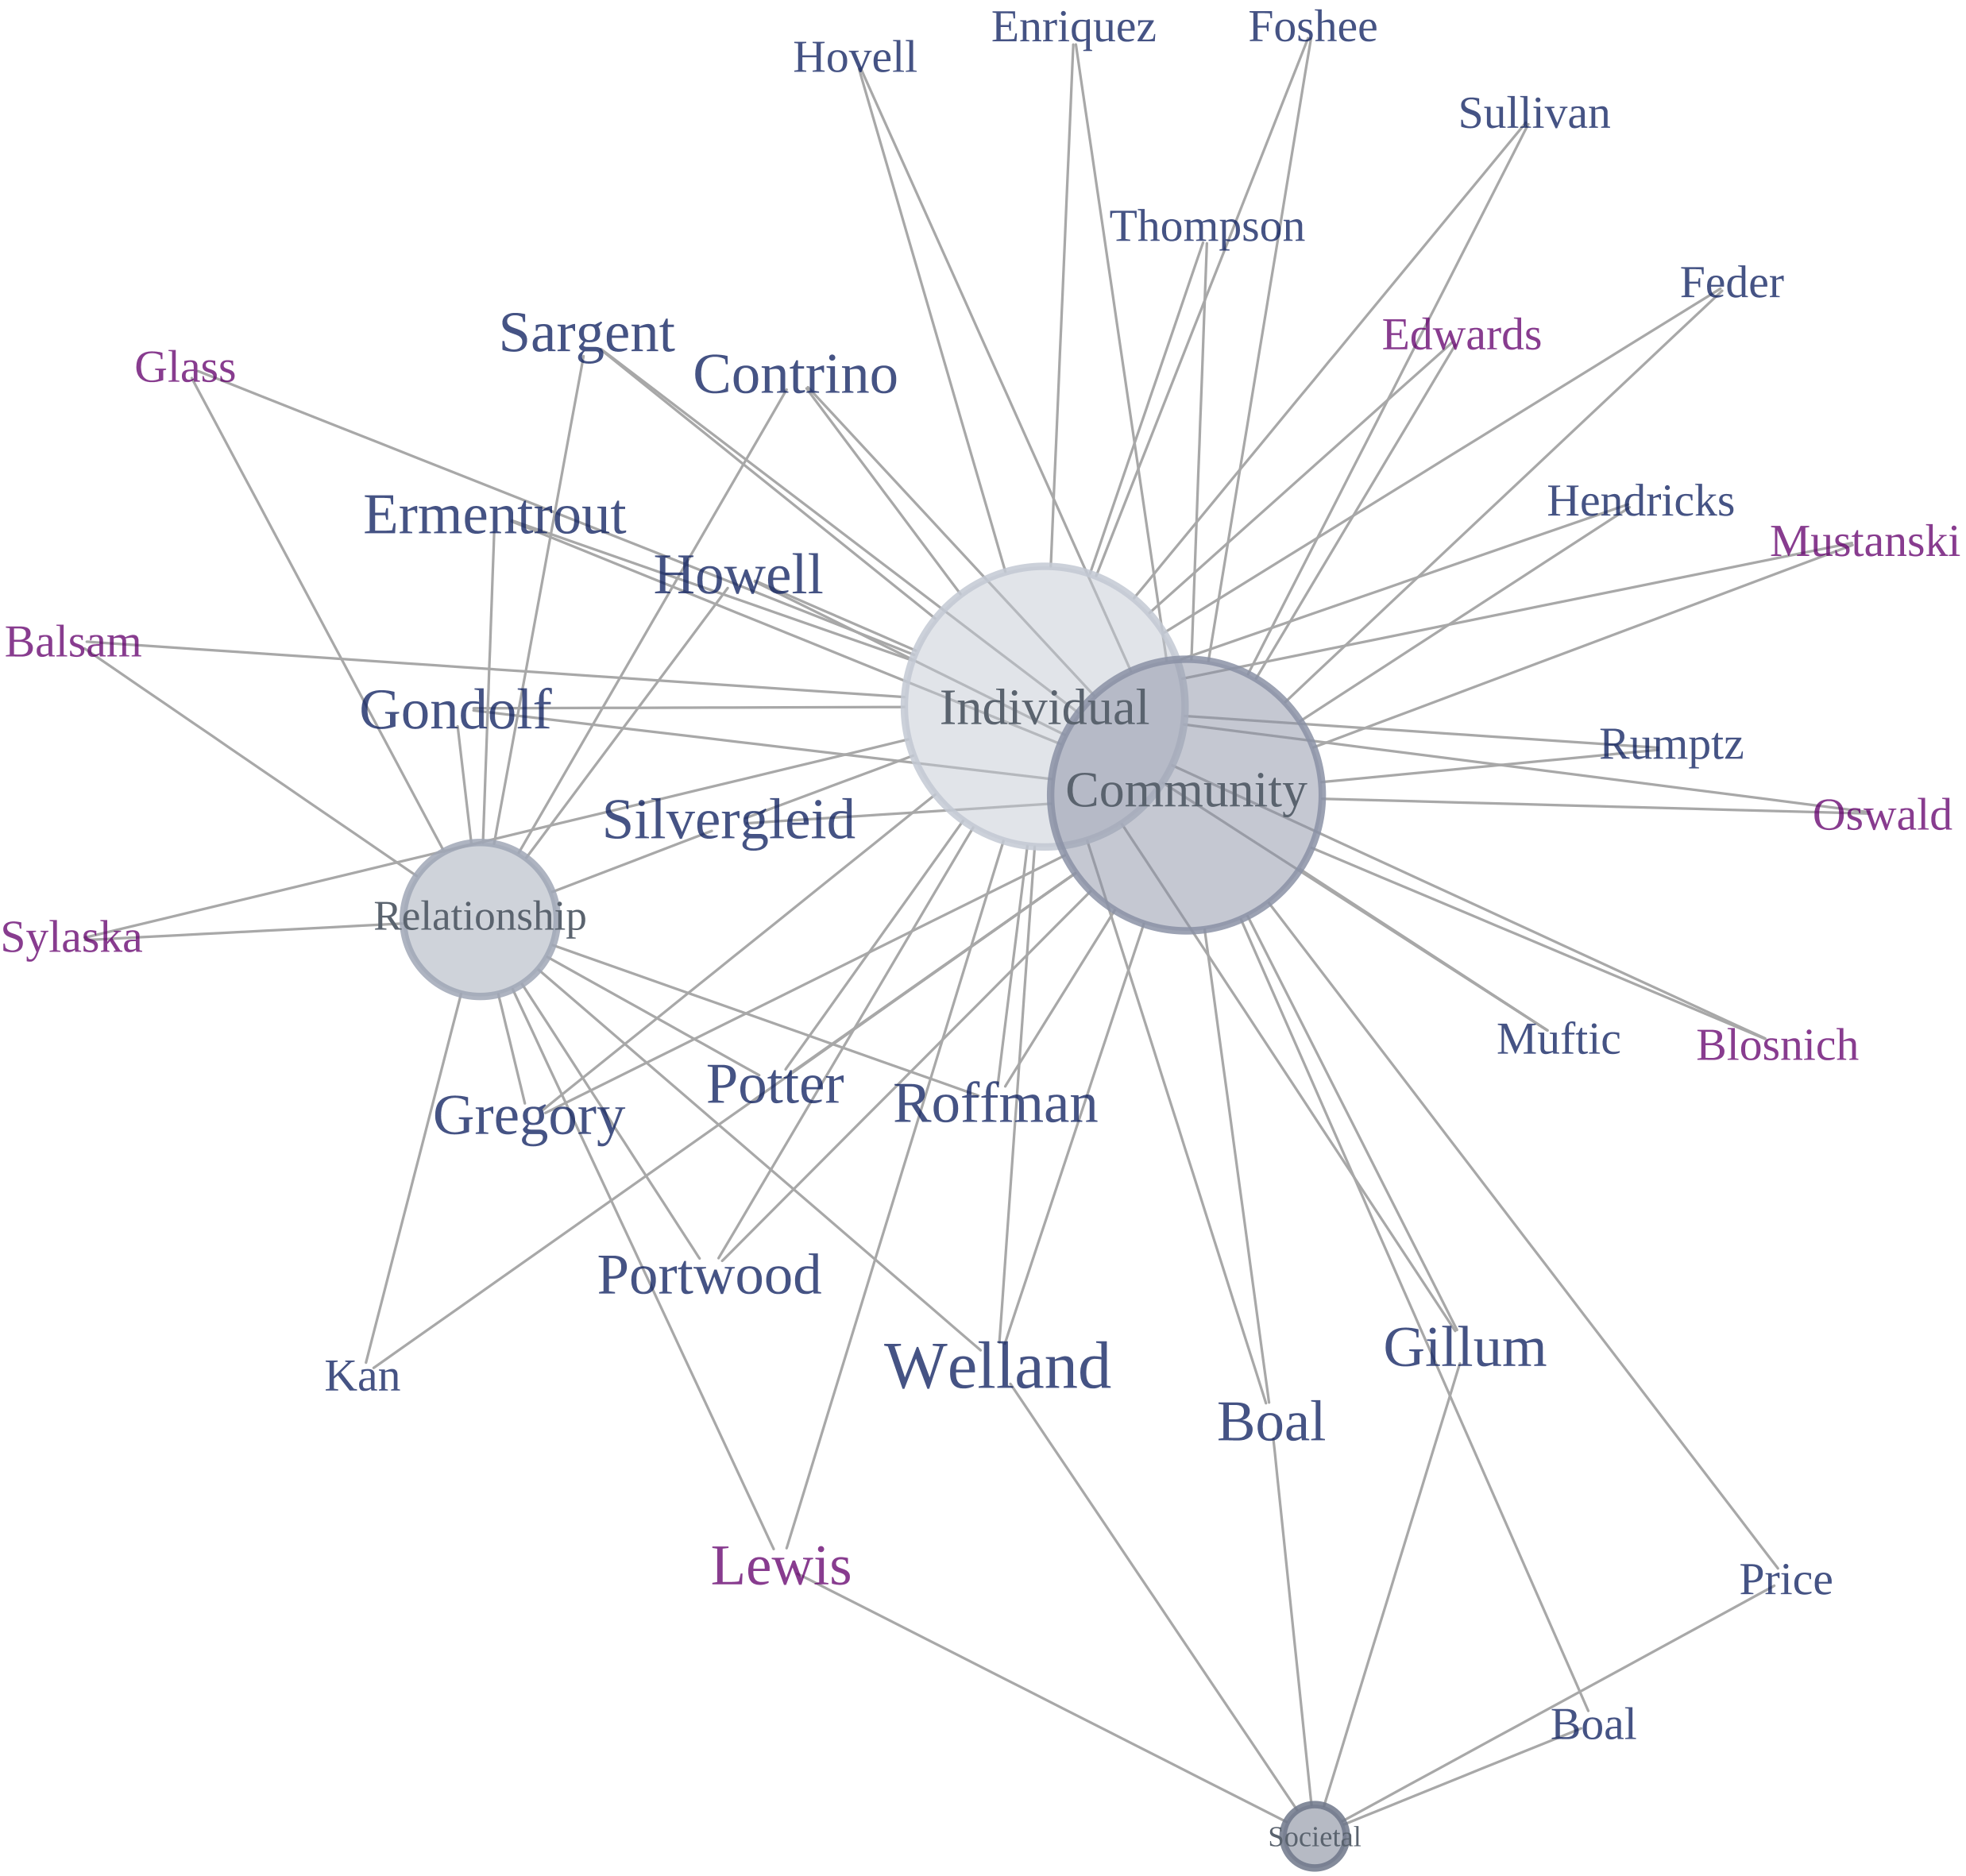
\includegraphics{graphics/inputs/keysnet.png}
\caption{Network graph of the levels of analysis involved in the
reviewed literature\label{fig:keysnet}}
\end{figure}

\newpage

\begin{figure}
\centering
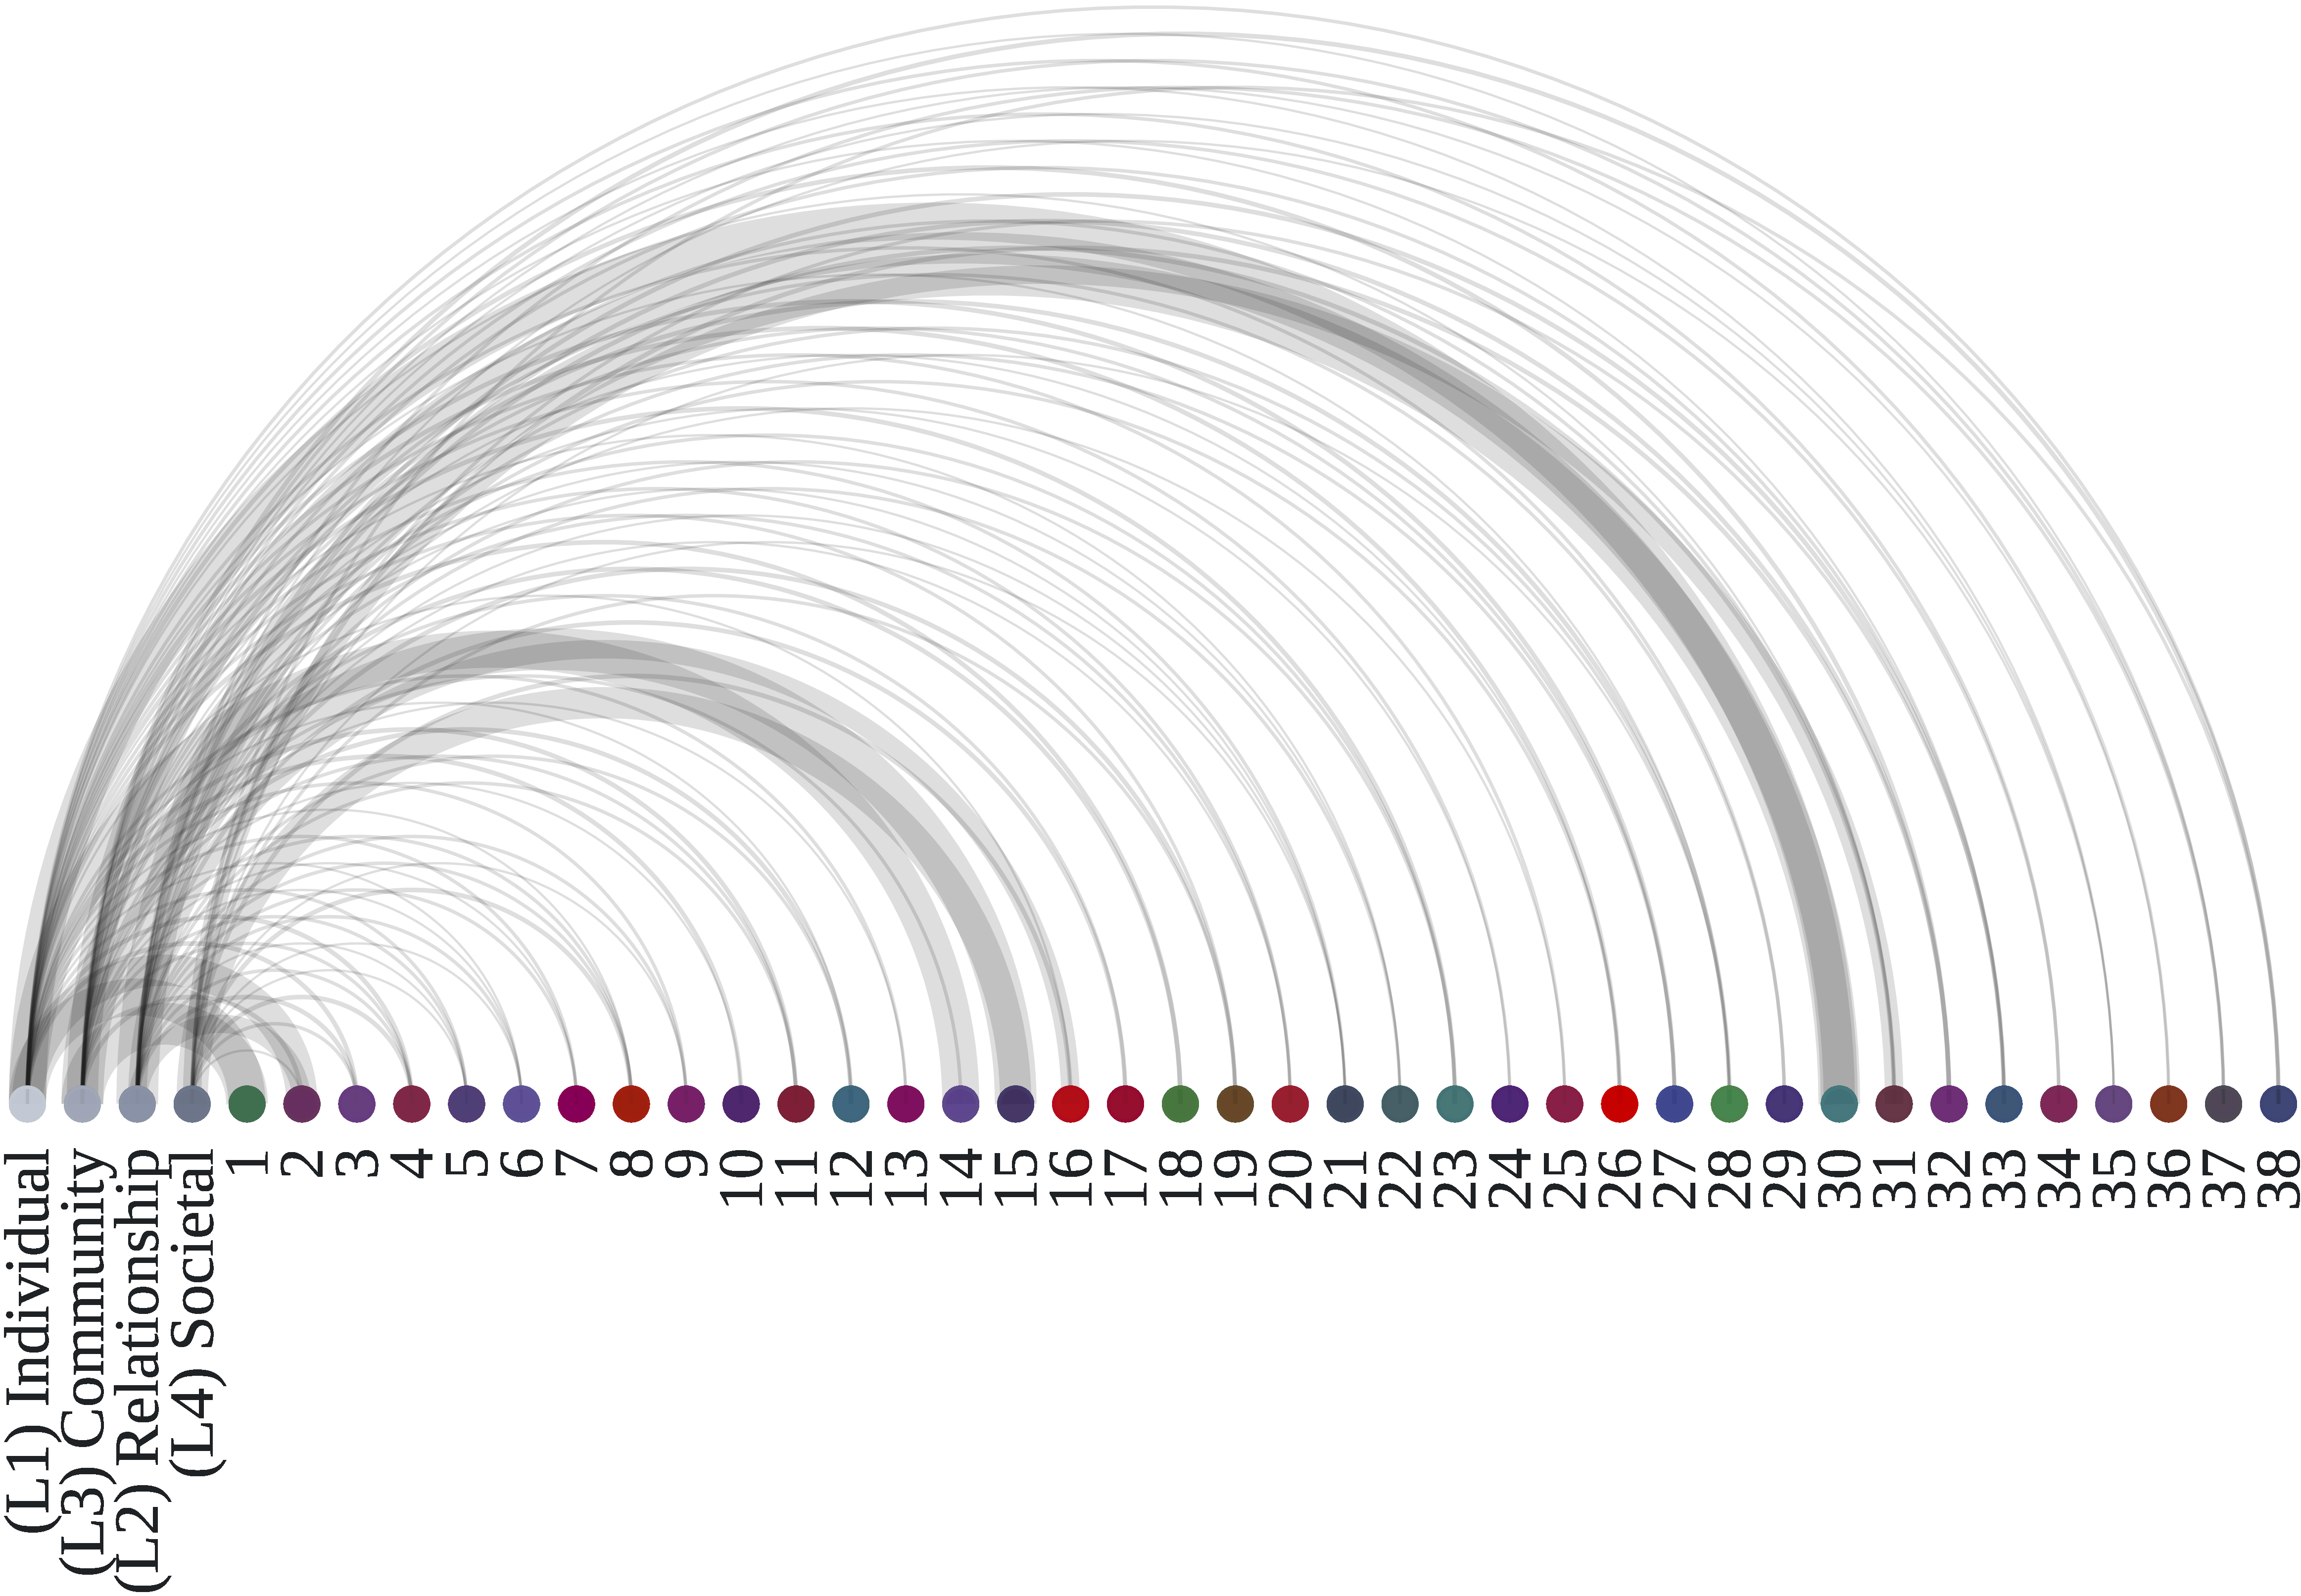
\includegraphics{graphics/inputs/arc_analyses.png}
\caption{Network Diagram Showing Relations among Analytic Approaches
(numbered graph nodes) used and Ecological Levels of Analysis (named
graph nodes) Invovled among the Reviewed Literature:
\textit{1 = Analysis of Covariance (ANCOVA), 2 = Analysis of Variance (ANOVA), 3 = Boostrapping, 4 = Chi-Square Difference Test, 5 = Confirmatory Factor Analysis (CFA), 6 = Constant Comparative Analysis, 7 = Content Analysis, 8 = Correlations, 9 = Cross-Case Analysis, 10 = Descriptives, 11 = Full SEM (Measurement \& Structural Models), 12 = Grounded Theory (GT)-Based Analysis, 13 = Grouped Thematic Analysis, 14 = Indirect-Effects, 15 = Linear Regression, 16 = Logistic Regression, 17 = Maximum Likelihood Estimation (MLE), 18 = Mediation Analysis, 19 = Mixed-Effects Modeling (MEM), 20 = Moderation/Conditional Process Analysis, 21 = Multi-Level/Hierarchical Linear Modeling (MLM/HLM), 22 = Multivariate Analyses, 23 = Multivariate Analysis of Covariance (MANCOVA), 24 = Multivariate Analysis of Variance (MANOVA), 25 = Odds Ratios (OR), 26 = Ordinary Least Squares Regression, 27 = Path Analysis, 28 = Post-Hoc Comparisons, 29 = Qualitative Descriptive Analysis, 30 = Relative Risk Ratios (RRR), 31 = Repeated-Measures ANOVA/ANCOVA, 32 = Structural Equation Modeling (SEM), 33 = T-Tests (Mean Differences), 34 = Thematic Analysis, 35 = Weighted Least Squares (WLS) Estimation}\label{fig:arc_analyses}}
\end{figure}

\newpage

\begin{figure}
\centering
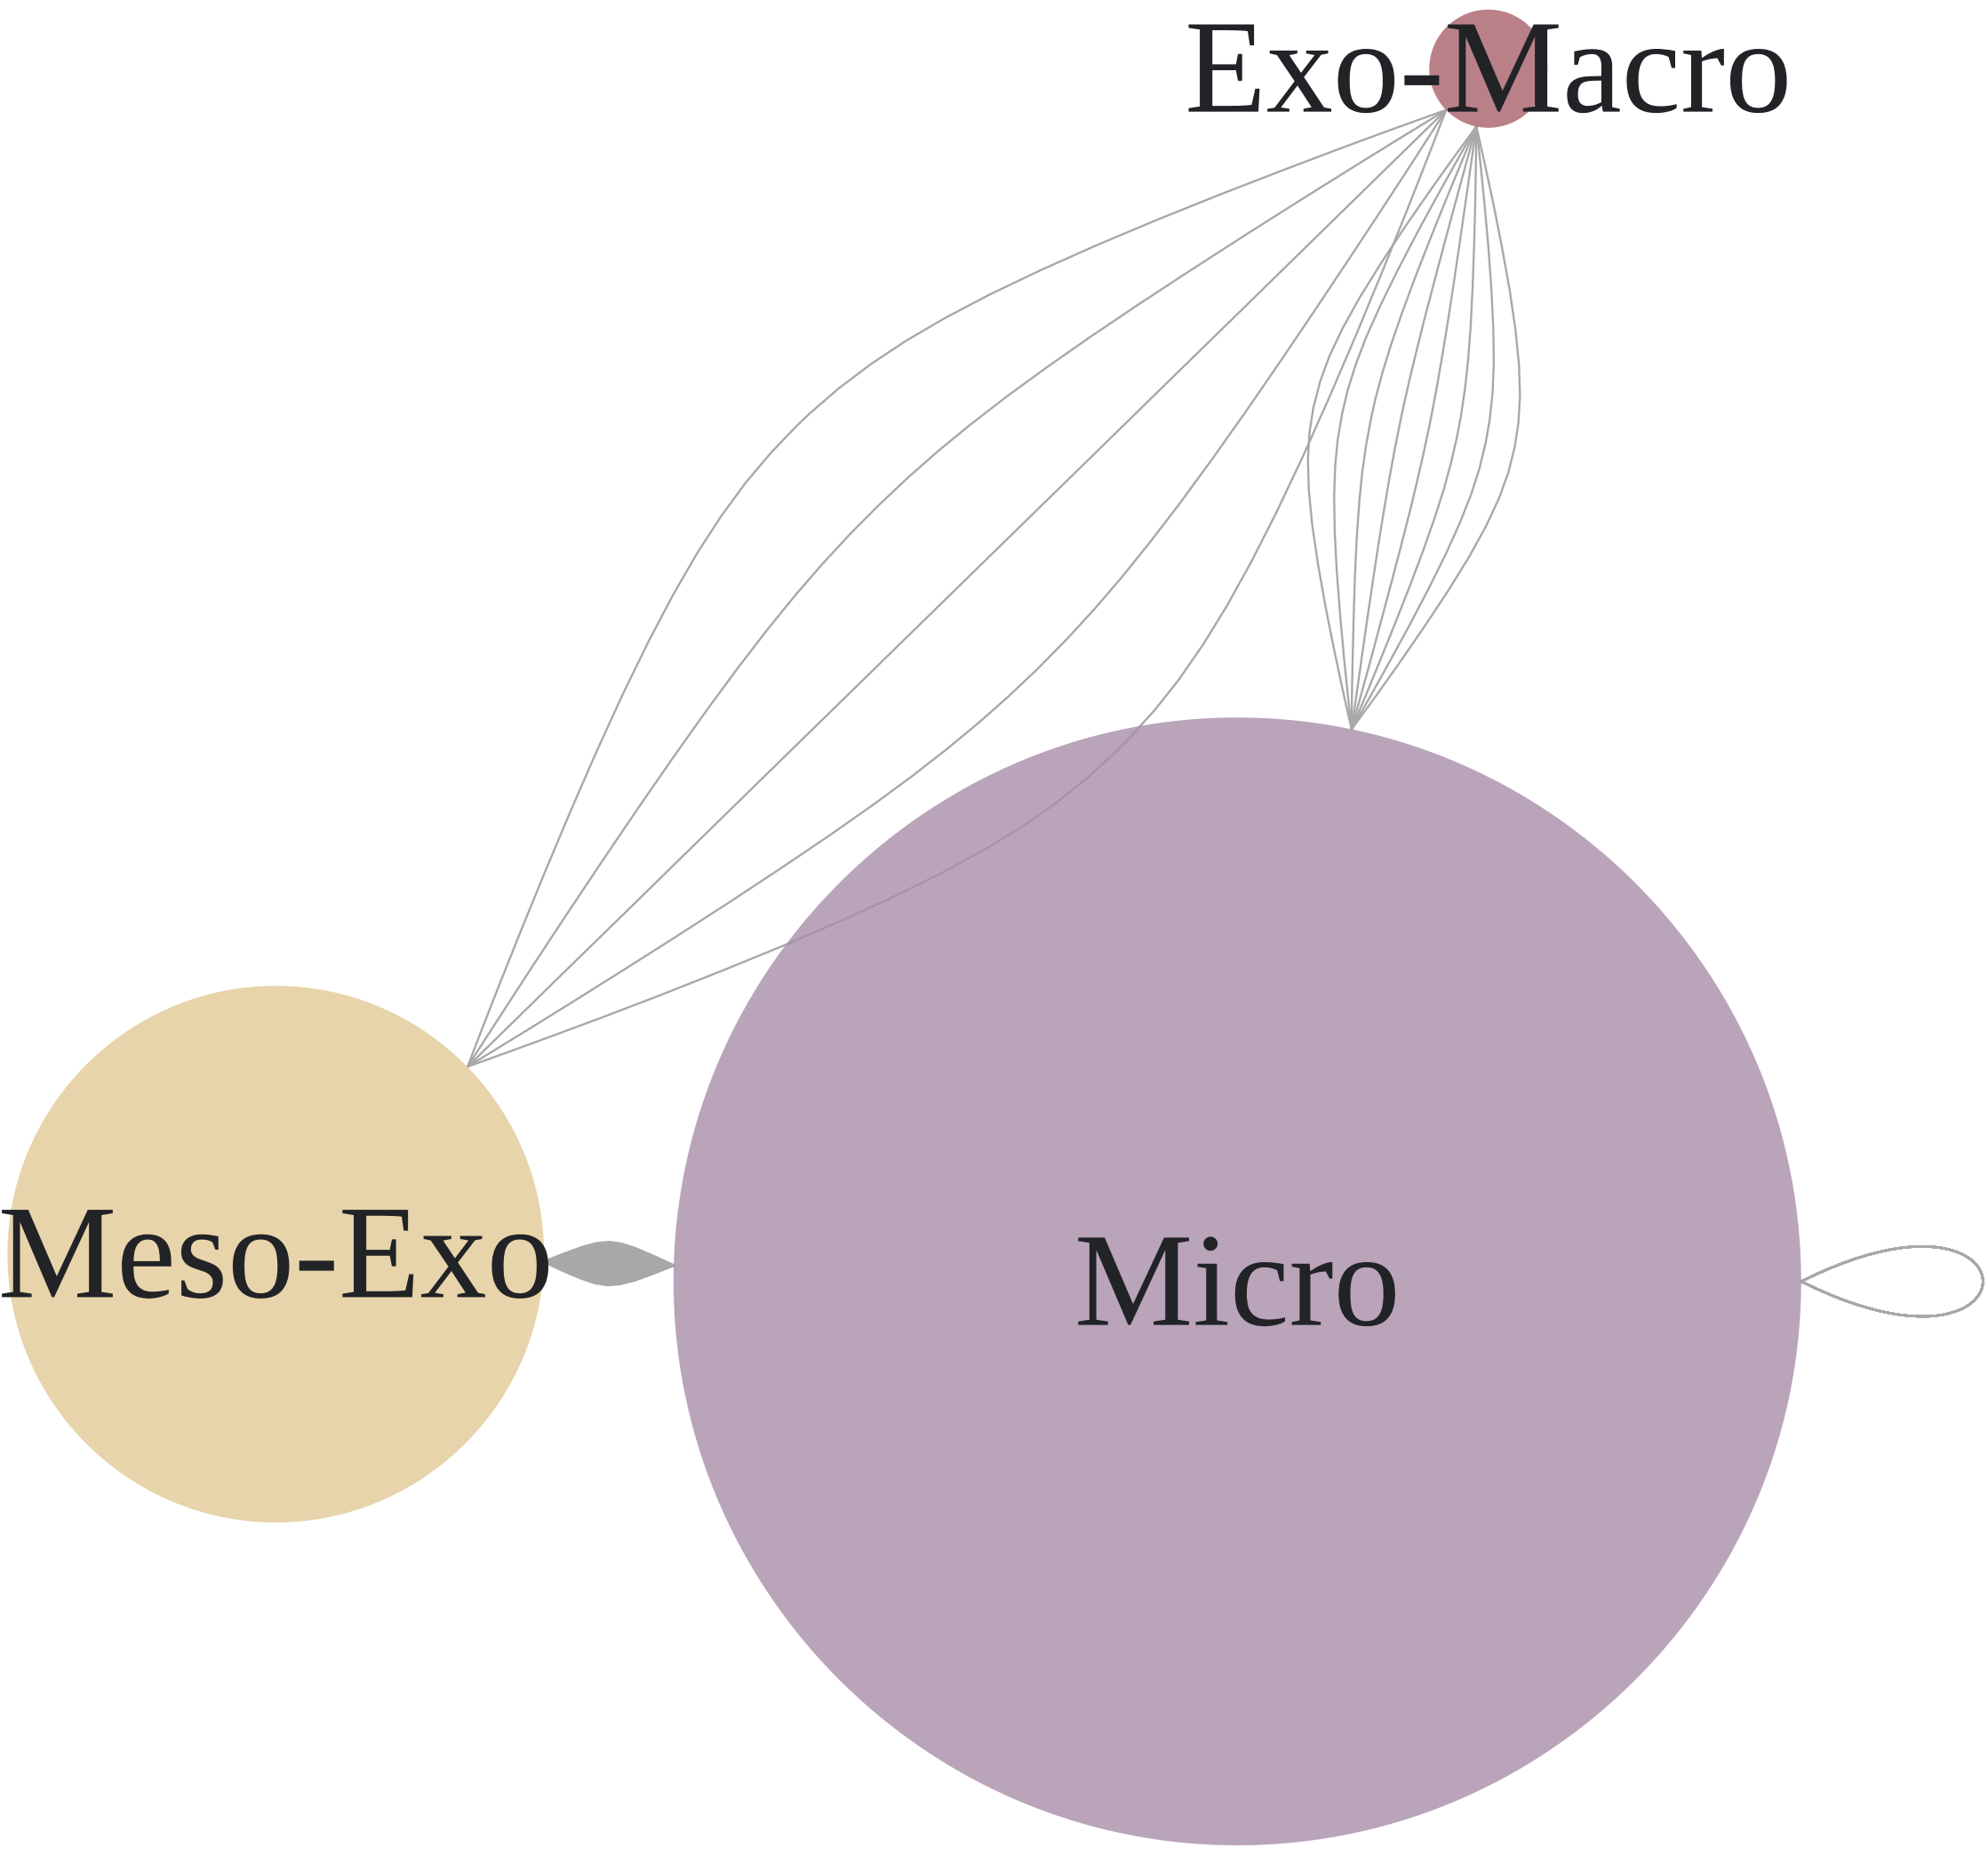
\includegraphics{graphics/inputs/sysnet.png}
\caption{Network Visualization Of The Ecological Systems Involved Across
The Reviewed Literature\label{fig:sysnet}}
\end{figure}

\newpage

\chapter{Appendix B. Literature Description \& Data Extraction
Template}\label{appendix-b.-literature-description-data-extraction-template}

\Frule

\chapter{Appendix C. Qualitative Comparative
Analysis}\label{appendix-c.-qualitative-comparative-analysis}

\part{References}

\refs

\hypertarget{refs}{}
\hypertarget{ref-andrews1994level}{}
Andrews, D., \& J. Bonta. (1995). \emph{Level of service
inventory--Revised (lsi--R)}. Toronto, Canada: Multi- Health Systems.

\hypertarget{ref-arias2013batterer}{}
Arias, E., R. Arce, \& M. Vilariño. (2013). Batterer intervention
programmes: A meta-analytic review of effectiveness. \emph{Psychosocial
Intervention}, \emph{22}, 153--160.

\hypertarget{ref-babcock2016domestic}{}
Babcock, J., N. Armenti, C. Cannon, K. Lauve-Moon, F. Buttell, R.
Ferreira, \ldots{} I. Solano. (2016). Domestic violence perpetrator
programs: A proposal for evidence-based standards in the united states.
\emph{Partner Abuse}, \emph{7}, 355--460.

\hypertarget{ref-baker2013lessons}{}
Baker, N., J. Buick, S. Kim, S. Moniz, \& K. L. Nava. (2013). Lessons
from examining same-sex intimate partner violence. \emph{Sex Roles},
\emph{69}, 182--192.

\hypertarget{ref-balcazar2004participatory}{}
Balcazar, F. E., R. R. Taylor, G. W. Kielhofner, K. Tamley, T. Benziger,
N. Carlin, \& S. Johnson. (2004). Participatory action research: General
principles and a study with a chronic health condition.

\hypertarget{ref-balsam2005relationship}{}
Balsam, K. F., \& D. M. Szymanski. (2005). Relationship quality and
domestic violence in women's same-sex relationships: The role of
minority stress. \emph{Psychology of Women Quarterly}, \emph{29},
258--269.

\hypertarget{ref-barker1964ecological}{}
Barker, R. G. (1964). The ecological environment. In R. G. Barker \& P.
V. Gump (Eds.), \emph{Big school, small school} (pp. pp. 4--10).
Stanford, CA: Stanford University Press.

\hypertarget{ref-black2011national}{}
Black, M. C., K. C. Basile, M. J. Breiding, S. G. Smith, M. L. Walters,
M. T. Merrick, \& M. Stevens. (2011). \emph{National Intimate Partner
And Sexual Violence Survey}. Atlanta, GA: Centers for Disease Control
and Prevention, National Center for Injury Prevention and Control.

\hypertarget{ref-blosnich2009comparisons}{}
Blosnich, J. R., \& R. M. Bossarte. (2009). Comparisons of intimate
partner violence among partners in same-sex and opposite-sex
relationships in the united states. \emph{American Journal of Public
Health}, \emph{99}, 2182--2184.

\hypertarget{ref-boal2014barriers}{}
Boal, A. L., \& E. S. Mankowski. (2014a). Barriers to compliance with
oregon batterer intervention program standards. \emph{Violence and
Victims}, \emph{29}, 607--619.

\hypertarget{ref-boal2014impact}{}
Boal, A. L., \& E. S. Mankowski. (2014b). The impact of legislative
standards on batterer intervention program practices and
characteristics. \emph{American Journal of Community Psychology},
\emph{53}, 218--230.

\hypertarget{ref-bronfenbrenner1977toward}{}
Bronfenbrenner, U. (1977). Toward an experimental ecology of human
development. \emph{American Psychologist}, \emph{32}, 513.

\hypertarget{ref-bronfenbrenner1979ecology}{}
Bronfenbrenner, U. (1979). \emph{The ecology of human development:
Experiments by nature and design}. Cambridge, MA: Harvard University
Press.

\hypertarget{ref-browning2002span}{}
Browning, C. R. (2002). The span of collective efficacy: Extending
social disorganization theory to partner violence. \emph{Journal of
Marriage and Family}, \emph{64}, 833--850.

\hypertarget{ref-brydon-miller2003why}{}
Brydon-Miller, M., D. Greenwood, \& P. Maguire. (2003). Why action
research? \emph{Action Research}, \emph{1}, 9--28.

\hypertarget{ref-burke1999violence}{}
Burke, L., \& D. R. Follingstad. (1999). Violence in lesbian and gay
relationships: Theory, prevalence, and correlational factors.
\emph{Clinical Psychology Review}, \emph{19}, 487--512.

\hypertarget{ref-cecere1986second}{}
Cecere, D. J. (1986). The second closet: Battered lesbians. \emph{Naming
the Violence: Speaking Out About Lesbian Battering}, 21--31.

\hypertarget{ref-centers2013taking}{}
Centers for Disease Control and Prevention. (2013). \emph{Taking action
to prevent intimate partner violence and sexual violence: Creating
statewide prevention plans}. Atlanta, GA: Centers for Disease Control;
Prevention, Division of Violence Prevention.

\hypertarget{ref-chandler2003transforming}{}
Chandler, D., \& B. Torbert. (2003). Transforming inquiry and action
interweaving 27 flavors of action research. \emph{Action Research},
\emph{1}, 133--152.

\hypertarget{ref-contrino2007compliance}{}
Contrino, K. M., K. H. Dermen, T. H. Nochajski, W. F. Wieczorek, \& P.
K. Navratil. (2007). Compliance and learning in an intervention program
for partner-violent men. \emph{Journal of Interpersonal Violence},
\emph{22}, 1555--1566.

\hypertarget{ref-dahlberg2002violence}{}
Dahlberg, L. L., \& E. G. Krug. (2002). Violence: A global public health
problem. In E. G. Krug, L. L. Dahlberg, J. A. Mercy, A. B. Zwi, \& R.
Lozano (Eds.), \emph{World report on violence and health} (pp. 1--21).
Geneva: World Health Organization.

\hypertarget{ref-dahlberg2009history}{}
Dahlberg, L. L., \& J. A. Mercy. (2009). History of violence as a public
health issue. \emph{AMA Virtual Mentor}, \emph{11}, 167--172. Retrieved
from \url{http://virtualmentor.ama-assn.org/2009/02/mhst1-0902.html}

\hypertarget{ref-durish2011documenting}{}
Durish, P. (2011). Documenting the same sex abuse project, toronto,
canada. In J. L. Ristock (Ed.), \emph{Intimate partner violence in LGBTQ
lives} (p. 232). New York, NY: Routledge.

\hypertarget{ref-dutton2006transforming}{}
Dutton, D. G., \& K. Corvo. (2006). Transforming a flawed policy: A call
to revive psychology and science in domestic violence research and
practice. \emph{Aggression and Violent Behavior}, \emph{11}, 457--483.

\hypertarget{ref-dutton2007duluth}{}
Dutton, D. G., \& K. Corvo. (2007). The duluth model: A data-impervious
paradigm and a failed strategy. \emph{Aggression and Violent Behavior},
\emph{12}, 658--667.

\hypertarget{ref-eckhardt2013effectiveness}{}
Eckhardt, C. I., C. M. Murphy, D. J. Whitaker, J. Sprunger, R. Dykstra,
\& K. Woodard. (2013). The effectiveness of intervention programs for
perpetrators and victims of intimate partner violence. \emph{Partner
Abuse}, \emph{4}, 196--231.

\hypertarget{ref-edelen2009measurement}{}
Edelen, M. O., D. F. McCaffrey, G. N. Marshall, \& L. H. Jaycox. (2009).
Measurement of teen dating violence attitudes an item response theory
evaluation of differential item functioning according to gender.
\emph{Journal of Interpersonal Violence}, \emph{24}, 1243--1263.

\hypertarget{ref-edwards2016college}{}
Edwards, K. M., H. L. Littleton, K. M. Sylaska, A. L. Crossman, \& M.
Craig. (2016). College campus community readiness to address intimate
partner violence among LGBTQ+ young adults: A conceptual and empirical
examination. \emph{American Journal of Community Psychology}, \emph{58},
16--26.

\hypertarget{ref-enriquez2010development}{}
Enriquez, M., A.-L. Cheng, P. J. Kelly, J. Witt, A. D. Coker, \& S.
Kashubeck-West. (2010). Development and feasibility of an hiv and ipv
prevention intervention among low-income mothers receiving services in a
missouri day care center. \emph{Violence Against Women}, \emph{16},
560--578.

\hypertarget{ref-ermentrout2014this}{}
Ermentrout, D. M., C. F. Rizo, \& R. J. Macy. (2014). ``This is about
me'': Feasibility findings from the children's component of an ipv
intervention for justice-involved families. \emph{Violence Against
Women}, \emph{20}, 653--676.

\hypertarget{ref-espino2008spirit}{}
Espino, S. L. R., \& E. J. Trickett. (2008). The spirit of ecological
inquiry and intervention research reports: A heuristic elaboration.
\emph{American Journal of Community Psychology}, \emph{42}, 60--78.

\hypertarget{ref-feder2005meta}{}
Feder, L., \& D. B. Wilson. (2005). A meta-analytic review of
court-mandated batterer intervention programs: Can courts affect
abusers' behavior? \emph{Journal of Experimental Criminology}, \emph{1},
239--262.

\hypertarget{ref-feder2011need}{}
Feder, L., P. H. Niolon, J. Campbell, J. Wallinder, R. Nelson, \& H.
Larrouy. (2011). The need for experimental methodology in intimate
partner violence: Finding programs that effectively prevent ipv.
\emph{Violence Against Women}, \emph{17}, 340--358.

\hypertarget{ref-fine1998violence}{}
Fine, D. M. (1998). Violence against women act of 1994: The proper
federal role in policing domestic violence. \emph{Cornell L. Rev.},
\emph{84}, 252--355.

\hypertarget{ref-fine2003participatory}{}
Fine, M., M. E. Torre, K. Boudin, I. Bowen, J. Clark, D. Hylton,
\ldots{} others. (2003). Participatory action research: From within and
beyond prison bars. In P. Camic, J. Rhodes, \& L. Yardley (Eds.),
\emph{Qualitative research in psychology: Expanding perspectives in
methodology and design} (pp. 179--198). Washington, DC, US: American
Psychological Association.

\hypertarget{ref-foshee2004assessing}{}
Foshee, V. A., K. E. Bauman, S. T. Ennett, G. F. Linder, T. Benefield,
\& C. Suchindran. (2004). Assessing the long-term effects of the safe
dates program and a booster in preventing and reducing adolescent dating
violence victimization and perpetration. \emph{American Journal of
Public Health}, \emph{94}, 619--624.

\hypertarget{ref-friedman-nimz2006blending}{}
Friedman-Nimz, R., J. Altman, S. Cain, S. Korn, M. J. Karger, M. Witsch,
\ldots{} M. Weiss. (2006). Blending support and social action: The power
of a gay-straight alliance and PrideWorks conference. \emph{Prufrock
Journal}, \emph{17}, 258--264.

\hypertarget{ref-fryer2008some}{}
Fryer, D. (2008). Some questions about ``the history of community
psychology''. \emph{Journal of Community Psychology}, \emph{36},
572--586.

\hypertarget{ref-gelles2001standards}{}
Gelles, R. J. (2001). Standards for programs for men who batter? Not
yet. \emph{Journal of Aggression, Maltreatment \& Trauma}, \emph{5},
11--20.

\hypertarget{ref-gilbert2002discourses}{}
Gilbert, P. R. (2002). Discourses of female violence and societal gender
stereotypes. \emph{Violence Against Women}, \emph{8}, 1271--1300.

\hypertarget{ref-gillum2008benefits}{}
Gillum, T. L. (2008). The benefits of a culturally specific intimate
partner violence intervention for african american survivors.
\emph{Violence Against Women}, \emph{14}, 917--943.

\hypertarget{ref-girshick2002no}{}
Girshick, L. B. (2002). No sugar, no spice: Reflections on research on
woman-to-woman sexual violence. \emph{Violence Against Women}, \emph{8},
1500--1520.

\hypertarget{ref-glass2008risk}{}
Glass, N., N. Perrin, G. Hanson, T. Bloom, E. Gardner, \& J. C.
Campbell. (2008). Risk for reassault in abusive female same-sex
relationships. \emph{American Journal of Public Health}, \emph{98},
1021--1027.

\hypertarget{ref-gondolf1999comparison}{}
Gondolf, E. W. (1999). A comparison of four batterer intervention
systems: Do court referral, program length, and services matter?
\emph{Journal of Interpersonal Violence}, \emph{14}, 41--61.

\hypertarget{ref-gondolf2007theoretical}{}
Gondolf, E. W. (2007). Theoretical and research support for the duluth
model: A reply to dutton and corvo. \emph{Aggression and Violent
Behavior}, \emph{12}, 644--657.

\hypertarget{ref-gondolf2009clinician}{}
Gondolf, E. W., \& H. Wernik. (2009). Clinician ratings of batterer
treatment behaviors in predicting reassault. \emph{Journal of
Interpersonal Violence}, \emph{24}, 1792--1815.

\hypertarget{ref-gregory2002effects}{}
Gregory, C., \& E. Erez. (2002). The effects of batterer intervention
programs: The battered women's perspectives. \emph{Violence Against
Women}, \emph{8}, 206--232.

\hypertarget{ref-hammond1989lesbian}{}
Hammond, N. (1989). Lesbian victims of relationship violence.
\emph{Women and Therapy}, \emph{8}, 89--105.

\hypertarget{ref-hart1986lesbian}{}
Hart, B. (1986). Lesbian battering: An examination. \emph{Naming the
Violence: Speaking Out About Lesbian Battering}, 173--189.

\hypertarget{ref-hart1995coordinated}{}
Hart, B. J. (1995, March). Coordinated community approaches to domestic
violence. Paper Presented at the Strategic Planning Workshop on Violence
Against Women, Washington, DC: National Institute of Justice. Retrieved
from
\url{http://www.ncdsv.org/images/Coordinated\%20Community\%20Approaches\%20to\%20DV.pdf}

\hypertarget{ref-hassouneh2008influence}{}
Hassouneh, D., \& N. Glass. (2008). The influence of gender role
stereotyping on women's experiences of female same-sex intimate partner
violence. \emph{Violence Against Women}, \emph{14}, 310--325.

\hypertarget{ref-hegarty1999multidimensional}{}
Hegarty, K., M. Sheehan, \& C. Schonfeld. (1999). A multidimensional
definition of partner abuse: Development and preliminary validation of
the composite abuse scale. \emph{Journal of Family Violence}, \emph{14},
399--415.

\hypertarget{ref-heise1998violence}{}
Heise, L. L. (1998). Violence against women an integrated, ecological
framework. \emph{Violence Against Women}, \emph{4}, 262--290.

\hypertarget{ref-hendricks2006recidivism}{}
Hendricks, B., T. Werner, L. Shipway, \& G. J. Turinetti. (2006).
Recidivism among spousal abusers: Predictions and program evaluation.
\emph{Journal of Interpersonal Violence}, \emph{21}, 703--716.

\hypertarget{ref-higgins2011cochrane}{}
Higgins, J., \& S. Green (Eds.). (2011). \emph{Cochrane handbook for
systematic reviews of interventions version 5.1.0 {[}updated march
2011{]}}. London, UK: The Cochrane Collaboration. Retrieved from
\url{http://handbook.cochrane.org}

\hypertarget{ref-hovell2006evaluation}{}
Hovell, M. F., A. G. Seid, \& S. Liles. (2006). Evaluation of a police
and social services domestic violence program: Empirical evidence needed
to inform public health policies. \emph{Violence Against Women},
\emph{12}, 137--159.

\hypertarget{ref-howell2015strengthening}{}
Howell, K. H., L. E. Miller, M. M. Lilly, V. Burlaka, A. Grogan-Kaylor,
\& S. Graham-Bermann. (2015). Strengthening positive parenting through
intervention: Evaluating the moms' empowerment program for women
experiencing intimate partner violence. \emph{Journal of Interpersonal
Violence}, \emph{30}, 232--252.

\hypertarget{ref-ingram2012nchs}{}
Ingram, D., \& S. Franco. (2012). NCHS urban-rural classification scheme
for counties. In \emph{Vital and health statistics} (Vol. 2).
Hyattsville, Maryland: National Center for Health Statistics, Centers
for Disease Control; Prevention.

\hypertarget{ref-kan2014can}{}
Kan, M. L., \& M. E. Feinberg. (2014). Can a family-focused,
transition-to-parenthood program prevent parent and partner aggression
among couples with young children? \emph{Violence and Victims},
\emph{29}, 967--980.

\hypertarget{ref-kelly1977social}{}
Kelly, J. G., L. R. Snowden, \& R. F. Munoz. (1977). Social and
community interventions. \emph{Annual Review of Psychology}, \emph{28},
323--361.

\hypertarget{ref-kelly2004community}{}
Kelly, J., S. Azelton, C. Lardon, L. Mock, D. Tandon, \& M. Thomas.
(2004). On community leadership: Stories about collaboration in action
research. \emph{American Journal of Community Psychology}, \emph{33},
205--216.

\hypertarget{ref-kloos2012community}{}
Kloos, B., J. Hill, E. Thomas, A. Wandersman, \& M. J. Elias. (2012).
\emph{Community psychology: Linking individuals and communities} (Third
Edition). Belmont, CA: Wadsworth, Cengage Learning.

\hypertarget{ref-krug2002world}{}
Krug, E. G., L. L. Dahlberg, J. A. Mercy, A. B. Zwi, \& R. Lozano
(Eds.). (2002). \emph{The world report on violence and health}. Geneva:
World Health Organization.

\hypertarget{ref-leech2007array}{}
Leech, N. L., \& A. J. Onwuegbuzie. (2007). An array of qualitative data
analysis tools: A call for data analysis triangulation. \emph{School
Psychology Quarterly}, \emph{22}, 557.

\hypertarget{ref-legates2001their}{}
LeGates, M. (2001). \emph{In their time: A history of feminism in
western society}. New York, NY: Routledge.

\hypertarget{ref-lewis2014sexual}{}
Lewis, R. J., R. J. Milletich, V. J. Derlega, \& M. A. Padilla. (2014).
Sexual minority stressors and psychological aggression in lesbian
women's intimate relationships: The mediating roles of rumination and
relationship satisfaction. \emph{Psychology of Women Quarterly},
\emph{38}, 535--550.

\hypertarget{ref-little2010perceptions}{}
Little, B., \& C. Terrance. (2010). Perceptions of domestic violence in
lesbian relationships: Stereotypes and gender role expectations.
\emph{Journal of Homosexuality}, \emph{57}, 429--440.

\hypertarget{ref-lobel1986naming}{}
Lobel, K. (1986). \emph{Naming the violence: Speaking out about lesbian
battering}. Seattle, WA, US: Seal Press.

\hypertarget{ref-lounsbury2009introduction}{}
Lounsbury, D. W., \& S. G. Mitchell. (2009). Introduction to special
issue on social ecological approaches to community health research and
action. \emph{American Journal of Community Psychology}, \emph{44},
213--220.

\hypertarget{ref-luke2005getting}{}
Luke, D. A. (2005). Getting the big picture in community science:
Methods that capture context. \emph{American Journal of Community
Psychology}, \emph{35}, 185.

\hypertarget{ref-maguire1987doing}{}
Maguire, P. (1987). \emph{Doing participatory research: A feminist
approach}. Amherst, MA: Center for International Education, School of
Education, University of Massachusetts.

\hypertarget{ref-maton2006community}{}
Maton, K. I., D. D. Perkins, D. G. Altman, L. Gutierrez, J. G. Kelly, J.
Rappaport, \& S. Saegert. (2006). Community-based interdisciplinary
research: Introduction to the special issue. \emph{American Journal of
Community Psychology}, \emph{38}, 1--7.

\hypertarget{ref-mcclennen2005domestic}{}
McClennen, J. (2005). Domestic violence between same-gender partners -
recent findings and future research. \emph{Journal of Interpersonal
Violence}, \emph{20}, 149--154.

\hypertarget{ref-mclaughlin2001knowledge}{}
McLaughlin, E., \& P. D. Rozee. (2001). Knowledge about heterosexual
versus lesbian battering among lesbians. \emph{Women and Therapy},
\emph{23}, 39--58.

\hypertarget{ref-messinger2011invisible}{}
Messinger, A. M. (2011). Invisible victims: Same-sex ipv in the national
violence against women survey. \emph{Journal of Interpersonal Violence},
\emph{26}, 2228--2243.

\hypertarget{ref-meyer1995minority}{}
Meyer, I. H. (1995). Minority stress and mental health in gay men.
\emph{Journal of Health and Social Behavior}, 38--56.

\hypertarget{ref-meyer2003prejudice}{}
Meyer, I. H. (2003). Prejudice, social stress, and mental health in
lesbian, gay, and bisexual populations: Conceptual issues and research
evidence. \emph{Psychological Bulletin}, \emph{129}, 674.

\hypertarget{ref-meyer2015resilience}{}
Meyer, I. H. (2015). Resilience in the study of minority stress and
health of sexual and gender minorities. \emph{Psychology of Sexual
Orientation and Gender Diversity}, \emph{2}, 209.

\hypertarget{ref-modi2014role}{}
Modi, M. N., S. Palmer, \& A. Armstrong. (2014). The role of violence
against women act in addressing intimate partner violence: A public
health issue. \emph{Journal of Women's Health}, \emph{23}, 253--259.

\hypertarget{ref-moher2009preferred}{}
Moher, D., A. Liberati, J. Tetzlaff, D. G. Altman, \& The PRISMA Group.
(2009). Preferred reporting items for systematic reviews and
meta-analyses: The PRISMA statement. \emph{PLoS med}, \emph{6},
e1000097.
\url{http://doi.org/https://doi.org/10.1371/journal.pmed.1000097}

\hypertarget{ref-muftic2007evaluation}{}
Mufti\(\acute{c}\), L. R., \& J. A. Bouffard. (2007). An evaluation of
gender differences in the implementation and impact of a comprehensive
approach to domestic violence. \emph{Violence Against Women}, \emph{13},
46--69.

\hypertarget{ref-mustanski2014syndemic}{}
Mustanski, B., R. Andrews, A. Herrick, R. Stall, \& P. W. Schnarrs.
(2014). A syndemic of psychosocial health disparities and associations
with risk for attempting suicide among young sexual minority men.
\emph{American Journal of Public Health}, \emph{104}, 287--294.

\hypertarget{ref-centers2015social}{}
National Center for Injury Prevention and Control. (2015). The
Social-Ecological Model: A framework for prevention. Atlanta, GA:
Centers for Disease Control and Prevention; Division of Violence and
Injury Prevention. Retrieved from
\url{https://www.cdc.gov/violenceprevention/pdf/sem_framewrk-a.pdf}

\hypertarget{ref-noffke1997professional}{}
Noffke, S. E. (1997). Professional, personal, and political dimensions
of action research. \emph{Review of Research in Education}, 305--343.

\hypertarget{ref-onwuegbuzie2017framework}{}
Onwuegbuzie, A. J., \& R. K. Weinbaum. (2017). A framework for using
qualitative comparative analysis for the review of the literature.
\emph{The Qualitative Report}, \emph{22}, 359--372.

\hypertarget{ref-onwuegbuzie2009qualitative}{}
Onwuegbuzie, A. J., W. B. Dickinson, N. L. Leech, \& A. G. Zoran.
(2009). A qualitative framework for collecting and analyzing data in
focus group research. \emph{International Journal of Qualitative
Methods}, \emph{8}, 1--21.

\hypertarget{ref-oswald2010lesbian}{}
Oswald, R. F., C. A. Fonseca, \& J. L. Hardesty. (2010). Lesbian
mothers' counseling experiences in the context of intimate partner
violence. \emph{Psychology of Women Quarterly}, \emph{34}, 286--296.

\hypertarget{ref-pence1983duluth}{}
Pence, E. (1983). Duluth domestic abuse intervention project, the.
\emph{Hamline Rev.}, \emph{6}, 247.

\hypertarget{ref-portwood2011evaluation}{}
Portwood, S. G., R. G. Lambert, L. P. Abrams, \& E. B. Nelson. (2011).
An evaluation of the adults and children together (act) against violence
parents raising safe kids program. \emph{Journal of Primary Prevention},
\emph{32}, 147--160.

\hypertarget{ref-potter2011bringing}{}
Potter, S. J., \& J. G. Stapleton. (2011). Bringing in the target
audience in bystander social marketing materials for communities:
Suggestions for practitioners. \emph{Violence Against Women}, \emph{17},
797--812.

\hypertarget{ref-price2009batterer}{}
Price, B. J., \& A. Rosenbaum. (2009). Batterer intervention programs: A
report from the field. \emph{Violence and Victims}, \emph{24}, 757--770.

\hypertarget{ref-prilleltensky1997values}{}
Prilleltensky, I. (1997). Values, assumptions, and practices: Assessing
the moral implications of psychological discourse and action.
\emph{American Psychologist}, \emph{52}, 517.

\hypertarget{ref-prilleltensky2001value-based}{}
Prilleltensky, I. (2001). Value-based praxis in community psychology:
Moving toward social justice and social action. \emph{American Journal
of Community Psychology}, \emph{29}, 747--778.

\hypertarget{ref-R-base}{}
R Core Team. (2016). \emph{R: A language and environment for statistical
computing}. Vienna, Austria: R Foundation for Statistical Computing.
Retrieved from \url{https://www.R-project.org/}

\hypertarget{ref-rappaport1987terms}{}
Rappaport, J. (1987). Terms of empowerment/exemplars of prevention:
Toward a theory for community psychology. \emph{American Journal of
Community Psychology}, \emph{15}, 121--148.

\hypertarget{ref-riger1993what}{}
Riger, S. (1993). What's wrong with empowerment. \emph{American Journal
of Community Psychology}, \emph{21}, 279--292.

\hypertarget{ref-ristock2001decentering}{}
Ristock, J. L. (2001). Decentering heterosexuality: Responses of
feminist counselors to abuse in lesbian relationships. \emph{Women and
Therapy}, \emph{23}, 59--72.

\hypertarget{ref-ristock2011intimate}{}
Ristock, J. L. (2011). \emph{Intimate partner violence in LGBTQ lives}.
New York, NY: Routledge.

\hypertarget{ref-roffman2008mens}{}
Roffman, R. A., J. L. Edleson, C. Neighbors, L. Mbilinyi, \& D. Walker.
(2008). The men's domestic abuse check-up: A protocol for reaching the
nonadjudicated and untreated man who batters and who abuses substances.
\emph{Violence Against Women}, \emph{14}, 589--605.

\hypertarget{ref-rumptz1991ecological}{}
Rumptz, M. H., C. M. Sullivan, W. S. Davidson, \& J. Basta. (1991). An
ecological approach to tracking battered women over time. \emph{Violence
and Victims}, \emph{6}, 237--244.

\hypertarget{ref-sarason1972creation}{}
Sarason, S. B. (1972). \emph{The creation of settings and the future
societies}. San Francisco, CA: Jossey-Bass.

\hypertarget{ref-sargent2016evaluating}{}
Sargent, K. S., R. McDonald, N. L. Vu, \& E. N. Jouriles. (2016).
Evaluating an online program to help children exposed to domestic
violence: Results of two randomized controlled trials. \emph{Journal of
Family Violence}, \emph{31}, 647--654.

\hypertarget{ref-seidman2012emerging}{}
Seidman, E. (2012). An emerging action science of social settings.
\emph{American Journal of Community Psychology}, \emph{50}, 1--16.

\hypertarget{ref-senn2005you}{}
Senn, C. Y. (2005). You can change the world: Action, participatory, and
activist research. In F. Schneider, J. Gruman, \& L. Coutts (Eds.),
\emph{Applied social psychology: Understanding and addressing social
problems} (pp. 355--373). Thousand Oaks, CA: SAGE Publications, Inc.

\hypertarget{ref-silvergleid2006batterer}{}
Silvergleid, C. S., \& E. S. Mankowski. (2006). How batterer
intervention programs work: Participant and facilitator accounts of
processes of change. \emph{Journal of Interpersonal Violence},
\emph{21}, 139--159.

\hypertarget{ref-smith2011women}{}
Smith, C. (2011). Women who abuse their female intimate partners. In J.
L. Ristock (Ed.), \emph{Intimate partner violence in LGBTQ lives} (pp.
131--52). New York, NY: Routledge.

\hypertarget{ref-sullivan2002findings}{}
Sullivan, C. M., D. I. Bybee, \& N. E. Allen. (2002). Findings from a
community-based program for battered women and their children.
\emph{Journal of Interpersonal Violence}, \emph{17}, 915--936.

\hypertarget{ref-sylaska2015disclosure}{}
Sylaska, K. M., \& K. M. Edwards. (2015). Disclosure experiences of
sexual minority college student victims of intimate partner violence.
\emph{American Journal of Community Psychology}, \emph{55}, 326--335.

\hypertarget{ref-scra2017other}{}
The Society for Community Research and Action (SCRA). (2017). Other
journals relevant to community psychology. Retrieved from
\url{http://www.scra27.org/publications/other-journals-relevant-community-psychology/}

\hypertarget{ref-biden2014twenty}{}
The White House, Office of the Vice President, \& J. Biden. (2014). 1 is
2 many: Twenty years fighting violence against women and girls
{[}Official U.S. White House report prepared by the Office of the Vice
President to commemorate the 20th Anniversary of the Violence Against
Women Act{]}. Washington, D.C., U.S.: Office of the Vice President, The
White House.

\hypertarget{ref-thompson2000identification}{}
Thompson, R. S., F. P. Rivara, D. C. Thompson, W. E. Barlow, N. K. Sugg,
R. D. Maiuro, \& D. M. Rubanowice. (2000). Identification and management
of domestic violence: A randomized trial. \emph{American Journal of
Preventive Medicine}, \emph{19}, 253--263.

\hypertarget{ref-tjaden2000full}{}
Tjaden, P., \& N. Thoennes. (2000). \emph{Full report of the prevalence,
incidence, and consequences of violence against women: Findings from the
National Violence against Women Survey: Research report}. Washington,
DC: National Institute of Justice.

\hypertarget{ref-tolman1995intervention}{}
Tolman, R., \& J. L. Edleson. (1995). Intervention for men who batter: A
review of research. \emph{Understanding Partner Violence: Prevalence,
Causes, Consequences, and Solutions}, \emph{11}, 262--273.

\hypertarget{ref-toro2005community}{}
Toro, P. A. (2005). Community psychology: Where do we go from here?
\emph{American Journal of Community Psychology}, \emph{35}, 9--16.

\hypertarget{ref-trickett2009community}{}
Trickett, E. J. (2009a). Community psychology: Individuals and
interventions in community context. \emph{Annual Review of Psychology},
\emph{60}, 395--419.

\hypertarget{ref-trickett2009multilevel}{}
Trickett, E. J. (2009b). Multilevel community-based culturally situated
interventions and community impact: An ecological perspective.
\emph{American Journal of Community Psychology}, \emph{43}, 257--266.

\hypertarget{ref-trickett2011water}{}
Trickett, E. J. (2011). From ``water boiling in a peruvian town'' to
``letting them die'': Culture, community intervention, and the metabolic
balance between patience and zeal. \emph{American Journal of Community
Psychology}, \emph{47}, 58--68.

\hypertarget{ref-walters2013national}{}
Walters, M. L., J. Chen, \& M. J. Breiding. (2013). \emph{The national
intimate partner and sexual violence survey (NISVS): 2010 findings on
victimization by sexual orientation}. Atlanta, GA: Centers for Disease
Control and Prevention.

\hypertarget{ref-welland2010culturally}{}
Welland, C., \& N. Ribner. (2010). Culturally specific treatment for
partner-abusive latino men: A qualitative study to identify and
implement program components. \emph{Violence and Victims}, \emph{25},
799--813.

\hypertarget{ref-whitaker2014linking}{}
Whitaker, P. (2014). Linking community protective factors to intimate
partner violence perpetration. \emph{Violence Against Women}, \emph{20},
1338--1359.

\hypertarget{ref-witte2015perceived}{}
Witte, T. H., M. M. Mulla, \& A. A. Weaver. (2015). Perceived social
norms for intimate partner violence in proximal and distal groups.
\emph{Violence and Victims}, \emph{30}, 691--698.



\end{document}
